% Options for packages loaded elsewhere
\PassOptionsToPackage{unicode}{hyperref}
\PassOptionsToPackage{hyphens}{url}
%
\documentclass[
]{article}
\usepackage{amsmath,amssymb}
\usepackage{iftex}
\ifPDFTeX
  \usepackage[T1]{fontenc}
  \usepackage[utf8]{inputenc}
  \usepackage{textcomp} % provide euro and other symbols
\else % if luatex or xetex
  \usepackage{unicode-math} % this also loads fontspec
  \defaultfontfeatures{Scale=MatchLowercase}
  \defaultfontfeatures[\rmfamily]{Ligatures=TeX,Scale=1}
\fi
\usepackage{lmodern}
\ifPDFTeX\else
  % xetex/luatex font selection
\fi
% Use upquote if available, for straight quotes in verbatim environments
\IfFileExists{upquote.sty}{\usepackage{upquote}}{}
\IfFileExists{microtype.sty}{% use microtype if available
  \usepackage[]{microtype}
  \UseMicrotypeSet[protrusion]{basicmath} % disable protrusion for tt fonts
}{}
\makeatletter
\@ifundefined{KOMAClassName}{% if non-KOMA class
  \IfFileExists{parskip.sty}{%
    \usepackage{parskip}
  }{% else
    \setlength{\parindent}{0pt}
    \setlength{\parskip}{6pt plus 2pt minus 1pt}}
}{% if KOMA class
  \KOMAoptions{parskip=half}}
\makeatother
\usepackage{xcolor}
\usepackage[margin=1in]{geometry}
\usepackage{color}
\usepackage{fancyvrb}
\newcommand{\VerbBar}{|}
\newcommand{\VERB}{\Verb[commandchars=\\\{\}]}
\DefineVerbatimEnvironment{Highlighting}{Verbatim}{commandchars=\\\{\}}
% Add ',fontsize=\small' for more characters per line
\usepackage{framed}
\definecolor{shadecolor}{RGB}{248,248,248}
\newenvironment{Shaded}{\begin{snugshade}}{\end{snugshade}}
\newcommand{\AlertTok}[1]{\textcolor[rgb]{0.94,0.16,0.16}{#1}}
\newcommand{\AnnotationTok}[1]{\textcolor[rgb]{0.56,0.35,0.01}{\textbf{\textit{#1}}}}
\newcommand{\AttributeTok}[1]{\textcolor[rgb]{0.13,0.29,0.53}{#1}}
\newcommand{\BaseNTok}[1]{\textcolor[rgb]{0.00,0.00,0.81}{#1}}
\newcommand{\BuiltInTok}[1]{#1}
\newcommand{\CharTok}[1]{\textcolor[rgb]{0.31,0.60,0.02}{#1}}
\newcommand{\CommentTok}[1]{\textcolor[rgb]{0.56,0.35,0.01}{\textit{#1}}}
\newcommand{\CommentVarTok}[1]{\textcolor[rgb]{0.56,0.35,0.01}{\textbf{\textit{#1}}}}
\newcommand{\ConstantTok}[1]{\textcolor[rgb]{0.56,0.35,0.01}{#1}}
\newcommand{\ControlFlowTok}[1]{\textcolor[rgb]{0.13,0.29,0.53}{\textbf{#1}}}
\newcommand{\DataTypeTok}[1]{\textcolor[rgb]{0.13,0.29,0.53}{#1}}
\newcommand{\DecValTok}[1]{\textcolor[rgb]{0.00,0.00,0.81}{#1}}
\newcommand{\DocumentationTok}[1]{\textcolor[rgb]{0.56,0.35,0.01}{\textbf{\textit{#1}}}}
\newcommand{\ErrorTok}[1]{\textcolor[rgb]{0.64,0.00,0.00}{\textbf{#1}}}
\newcommand{\ExtensionTok}[1]{#1}
\newcommand{\FloatTok}[1]{\textcolor[rgb]{0.00,0.00,0.81}{#1}}
\newcommand{\FunctionTok}[1]{\textcolor[rgb]{0.13,0.29,0.53}{\textbf{#1}}}
\newcommand{\ImportTok}[1]{#1}
\newcommand{\InformationTok}[1]{\textcolor[rgb]{0.56,0.35,0.01}{\textbf{\textit{#1}}}}
\newcommand{\KeywordTok}[1]{\textcolor[rgb]{0.13,0.29,0.53}{\textbf{#1}}}
\newcommand{\NormalTok}[1]{#1}
\newcommand{\OperatorTok}[1]{\textcolor[rgb]{0.81,0.36,0.00}{\textbf{#1}}}
\newcommand{\OtherTok}[1]{\textcolor[rgb]{0.56,0.35,0.01}{#1}}
\newcommand{\PreprocessorTok}[1]{\textcolor[rgb]{0.56,0.35,0.01}{\textit{#1}}}
\newcommand{\RegionMarkerTok}[1]{#1}
\newcommand{\SpecialCharTok}[1]{\textcolor[rgb]{0.81,0.36,0.00}{\textbf{#1}}}
\newcommand{\SpecialStringTok}[1]{\textcolor[rgb]{0.31,0.60,0.02}{#1}}
\newcommand{\StringTok}[1]{\textcolor[rgb]{0.31,0.60,0.02}{#1}}
\newcommand{\VariableTok}[1]{\textcolor[rgb]{0.00,0.00,0.00}{#1}}
\newcommand{\VerbatimStringTok}[1]{\textcolor[rgb]{0.31,0.60,0.02}{#1}}
\newcommand{\WarningTok}[1]{\textcolor[rgb]{0.56,0.35,0.01}{\textbf{\textit{#1}}}}
\usepackage{longtable,booktabs,array}
\usepackage{calc} % for calculating minipage widths
% Correct order of tables after \paragraph or \subparagraph
\usepackage{etoolbox}
\makeatletter
\patchcmd\longtable{\par}{\if@noskipsec\mbox{}\fi\par}{}{}
\makeatother
% Allow footnotes in longtable head/foot
\IfFileExists{footnotehyper.sty}{\usepackage{footnotehyper}}{\usepackage{footnote}}
\makesavenoteenv{longtable}
\usepackage{graphicx}
\makeatletter
\def\maxwidth{\ifdim\Gin@nat@width>\linewidth\linewidth\else\Gin@nat@width\fi}
\def\maxheight{\ifdim\Gin@nat@height>\textheight\textheight\else\Gin@nat@height\fi}
\makeatother
% Scale images if necessary, so that they will not overflow the page
% margins by default, and it is still possible to overwrite the defaults
% using explicit options in \includegraphics[width, height, ...]{}
\setkeys{Gin}{width=\maxwidth,height=\maxheight,keepaspectratio}
% Set default figure placement to htbp
\makeatletter
\def\fps@figure{htbp}
\makeatother
\setlength{\emergencystretch}{3em} % prevent overfull lines
\providecommand{\tightlist}{%
  \setlength{\itemsep}{0pt}\setlength{\parskip}{0pt}}
\setcounter{secnumdepth}{-\maxdimen} % remove section numbering
\ifLuaTeX
  \usepackage{selnolig}  % disable illegal ligatures
\fi
\IfFileExists{bookmark.sty}{\usepackage{bookmark}}{\usepackage{hyperref}}
\IfFileExists{xurl.sty}{\usepackage{xurl}}{} % add URL line breaks if available
\urlstyle{same}
\hypersetup{
  pdftitle={bartMan},
  hidelinks,
  pdfcreator={LaTeX via pandoc}}

\title{bartMan}
\author{}
\date{\vspace{-2.5em}}

\begin{document}
\maketitle

\hypertarget{introduction}{%
\section{Introduction}\label{introduction}}

Tree-based regression and classification has become a standard tool in
modern data science. Bayesian Additive Regression Trees
(BART)\footnote{Chipman, H. A., George, E. I., \& McCulloch, R. E.
  (2010). BART: Bayesian additive regression trees. \emph{The Annals of
  Applied Statistics}, 4(1), 266-298.} has in particular gained wide
popularity due its flexibility in dealing with interactions and
non-linear effects. BART is a Bayesian tree-based machine learning
method that can be applied to both regression and classification
problems and yields competitive or superior results when compared to
other predictive models. As a Bayesian model, BART allows the
practitioner to explore the uncertainty around predictions through the
posterior distribution. In the \texttt{bartMan} package, we present new
visualisation techniques for exploring BART models. We construct
conventional plots to analyze a model's performance and stability as
well as create new tree-based plots to analyze variable importance,
interaction, and tree structure. We employ Value Suppressing Uncertainty
Palettes (VSUP)\footnote{Correll, M., Moritz, D., \& Heer, J. (2018,
  April). Value-suppressing uncertainty palettes. In Proceedings of the
  2018 CHI Conference on Human Factors in Computing Systems (pp.~1-11).}
to construct heatmaps that display variable importance and interactions
jointly using color scale to represent posterior uncertainty. Our new
visualisations are designed to work with the most popular BART R
packages available, namely \texttt{BART}\footnote{Sparapani R, Spanbauer
  C, McCulloch R (2021). Nonparametric Machine Learning and Efficient
  Computation with Bayesian Additive Regression Trees: The BART R
  Package. \emph{Journal of Statistical Software}},
\texttt{dbarts}\footnote{Vincent Dorie, dbarts: Discrete Bayesian
  Additive Regression Trees Sampler, 2020}, and
\texttt{bartMachine}\footnote{Adam Kapelner, Justin Bleich (2016).
  bartMachine: Machine Learning with Bayesian Additive Regression Trees.
  \emph{Journal of Statistical Software}}.

In this document, we demonstrate our visualisations for evaluation of
BART models using the \texttt{bartMan} (BART Model ANalysis) package.

\hypertarget{install-instructions}{%
\subsection{Install instructions}\label{install-instructions}}

To install the development version from GitHub, use:

\begin{Shaded}
\begin{Highlighting}[]
\CommentTok{\# install.packages("devtools")}
\CommentTok{\#devtools::install\_github("AlanInglis/bartMan")}
\FunctionTok{library}\NormalTok{(bartMan)}
\end{Highlighting}
\end{Shaded}

The data used in the following examples is simulated from the Friedman
benchmark problem 7\footnote{Friedman, Jerome H. (1991) Multivariate
  adaptive regression splines. \emph{The Annals of Statistics} 19 (1),
  pages 1-67.}. This benchmark problem is commonly used for testing
purposes. The output is created according to the equation:

\[y = 10 sin(π x_1 x_2) + 20 (x_3 - 0.5)^2 + 10 x_4 + 5 x_5 + e\]

\begin{Shaded}
\begin{Highlighting}[]
\DocumentationTok{\#\# Create Friedman data}
\NormalTok{fData  }\OtherTok{\textless{}{-}} \ControlFlowTok{function}\NormalTok{(}\AttributeTok{n =} \DecValTok{200}\NormalTok{, }\AttributeTok{sigma =} \FloatTok{1.0}\NormalTok{, }\AttributeTok{seed =} \DecValTok{1701}\NormalTok{, }\AttributeTok{nvar =} \DecValTok{5}\NormalTok{) \{}
  \FunctionTok{set.seed}\NormalTok{(seed)}
\NormalTok{  x }\OtherTok{\textless{}{-}} \FunctionTok{matrix}\NormalTok{(}\FunctionTok{runif}\NormalTok{(n }\SpecialCharTok{*}\NormalTok{ nvar), n, nvar)}
  \FunctionTok{colnames}\NormalTok{(x) }\OtherTok{\textless{}{-}} \FunctionTok{paste0}\NormalTok{(}\StringTok{"x"}\NormalTok{, }\DecValTok{1}\SpecialCharTok{:}\NormalTok{nvar)}
  
\NormalTok{  Ey }\OtherTok{\textless{}{-}} \DecValTok{10} \SpecialCharTok{*} \FunctionTok{sin}\NormalTok{(pi }\SpecialCharTok{*}\NormalTok{ x[, }\DecValTok{1}\NormalTok{] }\SpecialCharTok{*}\NormalTok{ x[, }\DecValTok{2}\NormalTok{]) }\SpecialCharTok{+} \DecValTok{20} \SpecialCharTok{*}\NormalTok{ (x[, }\DecValTok{3}\NormalTok{] }\SpecialCharTok{{-}} \FloatTok{0.5}\NormalTok{)}\SpecialCharTok{\^{}}\DecValTok{2} \SpecialCharTok{+} \DecValTok{10} \SpecialCharTok{*}\NormalTok{ x[, }\DecValTok{4}\NormalTok{] }\SpecialCharTok{+} \DecValTok{5} \SpecialCharTok{*}\NormalTok{ x[, }\DecValTok{5}\NormalTok{]}
\NormalTok{  y }\OtherTok{\textless{}{-}} \FunctionTok{rnorm}\NormalTok{(n, Ey, sigma)}
  
\NormalTok{  data }\OtherTok{\textless{}{-}} \FunctionTok{as.data.frame}\NormalTok{(}\FunctionTok{cbind}\NormalTok{(x, y))}
  \FunctionTok{return}\NormalTok{(data)}
\NormalTok{\}}

\NormalTok{f\_data }\OtherTok{\textless{}{-}} \FunctionTok{fData}\NormalTok{(}\AttributeTok{nvar =} \DecValTok{10}\NormalTok{)}
\NormalTok{x }\OtherTok{\textless{}{-}}\NormalTok{ f\_data[, }\DecValTok{1}\SpecialCharTok{:}\DecValTok{10}\NormalTok{]}
\NormalTok{y }\OtherTok{\textless{}{-}}\NormalTok{ f\_data}\SpecialCharTok{$}\NormalTok{y}
\end{Highlighting}
\end{Shaded}

Now we will create a basic BART model using the \texttt{dbarts} package.
However, the visualisation process outlined in this document is
identical for any of the \texttt{dbarts}, \texttt{BART}, or
\texttt{bartMachine} BART packages.

To begin we load the libraries and then create our models.

\begin{Shaded}
\begin{Highlighting}[]
\CommentTok{\# load libraries}
\FunctionTok{library}\NormalTok{(dbarts) }\CommentTok{\# for model}
\FunctionTok{library}\NormalTok{(ggplot2) }\CommentTok{\# for plots}
\end{Highlighting}
\end{Shaded}

\begin{Shaded}
\begin{Highlighting}[]

\CommentTok{\# create dbarts model:}
\FunctionTok{set.seed}\NormalTok{(}\DecValTok{1701}\NormalTok{)}
\NormalTok{dbartModel }\OtherTok{\textless{}{-}} \FunctionTok{bart}\NormalTok{(x,}
\NormalTok{                   y,}
                   \AttributeTok{ntree =} \DecValTok{5}\NormalTok{,}
                   \AttributeTok{keeptrees =} \ConstantTok{TRUE}\NormalTok{,}
                   \AttributeTok{nskip =} \DecValTok{10}\NormalTok{,}
                   \AttributeTok{ndpost =} \DecValTok{10}
\NormalTok{)}
\end{Highlighting}
\end{Shaded}

In \texttt{dbartModel} we have selected there to be 20 trees, 1000
iterations, and a burn-in of 100. Once the model is built we can extract
the data concerning the trees via the \texttt{extractTreeData} function.

\begin{Shaded}
\begin{Highlighting}[]
\CommentTok{\# Create data frames {-}{-}{-}{-}{-}{-}{-}{-}{-}{-}{-}{-}{-}{-}{-}{-}{-}{-}{-}{-}{-}{-}{-}{-}{-}{-}{-}{-}{-}{-}{-}{-}{-}{-}{-}{-}{-}{-}{-}{-}{-}{-}{-}{-}{-}{-}{-}{-}{-}{-}{-}{-}{-}{-}}
\NormalTok{trees\_data }\OtherTok{\textless{}{-}} \FunctionTok{extractTreeData}\NormalTok{(}\AttributeTok{model =}\NormalTok{ dbartModel, }\AttributeTok{data =}\NormalTok{ fData)}
\end{Highlighting}
\end{Shaded}

The object created by the \texttt{extractTreeData} function is a list
containing five elements. These are:

\begin{enumerate}
\def\labelenumi{\arabic{enumi}.}
\tightlist
\item
  \textbf{Tree Data Frame} - A data frame containing tree attributes.
\item
  \textbf{Variable Name} - The names of the variables used in building
  the model.
\item
  \textbf{nMCMC} - The total number of iterations (posterior draws)
  after burn in.
\item
  \textbf{nTree} - The total number of trees grown in the sum-of-trees
  model.
\item
  \textbf{nVar} - The total number of covariates used in the model.
\end{enumerate}

The tree data frame created from the \texttt{extractTreeData} function
contains 17 columns concerning different attributes associated with the
trees, and the structure of which is the same across all BART packages.
It can be accessed via \texttt{\$structure}. This data frame is used by
many of the \texttt{bartMan} functions to create the visualisations
shown later. In the code below, we take a look at the structure of the
data frame of trees.

\begin{Shaded}
\begin{Highlighting}[]
\FunctionTok{options}\NormalTok{(}\AttributeTok{tibble.width =} \ConstantTok{Inf}\NormalTok{) }\CommentTok{\# used to display full tibble in output}
\FunctionTok{head}\NormalTok{(trees\_data}\SpecialCharTok{$}\NormalTok{structure, }\DecValTok{5}\NormalTok{)}
\CommentTok{\#\textgreater{} \# A tibble: 5 x 17}
\CommentTok{\#\textgreater{}   var   splitValue terminal leafValue iteration treeNum  node childLeft}
\CommentTok{\#\textgreater{}   \textless{}chr\textgreater{}      \textless{}dbl\textgreater{} \textless{}lgl\textgreater{}        \textless{}dbl\textgreater{}     \textless{}int\textgreater{}   \textless{}int\textgreater{} \textless{}int\textgreater{}     \textless{}int\textgreater{}}
\CommentTok{\#\textgreater{} 1 x1         0.564 FALSE      NA              1       1     1         2}
\CommentTok{\#\textgreater{} 2 \textless{}NA\textgreater{}      NA     TRUE       {-}0.0209         1       1     2        NA}
\CommentTok{\#\textgreater{} 3 \textless{}NA\textgreater{}      NA     TRUE        0.0357         1       1     3        NA}
\CommentTok{\#\textgreater{} 4 x1         0.278 FALSE      NA              1       2     1         2}
\CommentTok{\#\textgreater{} 5 \textless{}NA\textgreater{}      NA     TRUE       {-}0.209          1       2     2        NA}
\CommentTok{\#\textgreater{}   childRight parent depth depthMax isStump label         value obsNode     noObs}
\CommentTok{\#\textgreater{}        \textless{}int\textgreater{}  \textless{}int\textgreater{} \textless{}dbl\textgreater{}    \textless{}dbl\textgreater{} \textless{}lgl\textgreater{}   \textless{}chr\textgreater{}         \textless{}dbl\textgreater{} \textless{}list\textgreater{}      \textless{}int\textgreater{}}
\CommentTok{\#\textgreater{} 1          3     NA     0        1 FALSE   x1  ≤  0.56  0.564  \textless{}dbl [200]\textgreater{}   200}
\CommentTok{\#\textgreater{} 2         NA      1     1        1 FALSE   {-}0.02       {-}0.0209 \textless{}dbl [107]\textgreater{}   107}
\CommentTok{\#\textgreater{} 3         NA      1     1        1 FALSE   0.04         0.0357 \textless{}dbl [93]\textgreater{}     93}
\CommentTok{\#\textgreater{} 4          3     NA     0        1 FALSE   x1  ≤  0.28  0.278  \textless{}dbl [200]\textgreater{}   200}
\CommentTok{\#\textgreater{} 5         NA      1     1        1 FALSE   {-}0.21       {-}0.209  \textless{}dbl [51]\textgreater{}     51}
\end{Highlighting}
\end{Shaded}

In the following table, each of the columns of
\texttt{trees\_data\$structure} are explained:

\begin{longtable}[]{@{}
  >{\raggedright\arraybackslash}p{(\columnwidth - 2\tabcolsep) * \real{0.1240}}
  >{\raggedright\arraybackslash}p{(\columnwidth - 2\tabcolsep) * \real{0.8760}}@{}}
\toprule\noalign{}
\begin{minipage}[b]{\linewidth}\raggedright
Column
\end{minipage} & \begin{minipage}[b]{\linewidth}\raggedright
Description
\end{minipage} \\
\midrule\noalign{}
\endhead
\bottomrule\noalign{}
\endlastfoot
\textbf{var} & Variable name used for splitting. \\
\textbf{splitValue} & Value of the variable at which the split
occurs. \\
\textbf{terminal} & Logical indicator if the node is terminal (TRUE) or
not (FALSE). \\
\textbf{leafValue} & Value at the leaf node, NA for non-terminal
nodes. \\
\textbf{iteration} & Iteration number. \\
\textbf{treeNum} & Tree number. \\
\textbf{node} & Unique identifier for the node (following
depth-first-left-side traversal). \\
\textbf{childLeft} & Identifier for the left child of the node, NA for
terminal nodes. \\
\textbf{childRight} & Identifier for the right child of the node, NA for
terminal nodes. \\
\textbf{parent} & Identifier for the parent of the node, NA for root
nodes. \\
\textbf{depth} & Depth of the node in the tree, starting from 0 for root
nodes. \\
\textbf{depthMax} & Maximum depth of the tree. \\
\textbf{isStump} & Logical indicator if the node is a stump (TRUE) or
not (FALSE). \\
\textbf{label} & Node label. \\
\textbf{value} & The value in a node (i.e., either the split value or
leaf value). \\
\textbf{obsNode} & List of observations in the node, represented in a
compact form. \\
\textbf{noObs} & Number of observations in the node. \\
\end{longtable}

As mentioned, the trees in the dataframe are ordered in a depth-first
left-side traversal method. An example of this is shown below in the
eample tree. Here we can see the ordering and node number used in this
method. Specifically, the \texttt{\$structure\$var} column would be
ordered as \texttt{X1,\ NA,\ X2,\ X2,\ \ NA,\ NA,\ NA}, where
\texttt{NA} indicates terminal (or leaf) nodes.

\begin{center}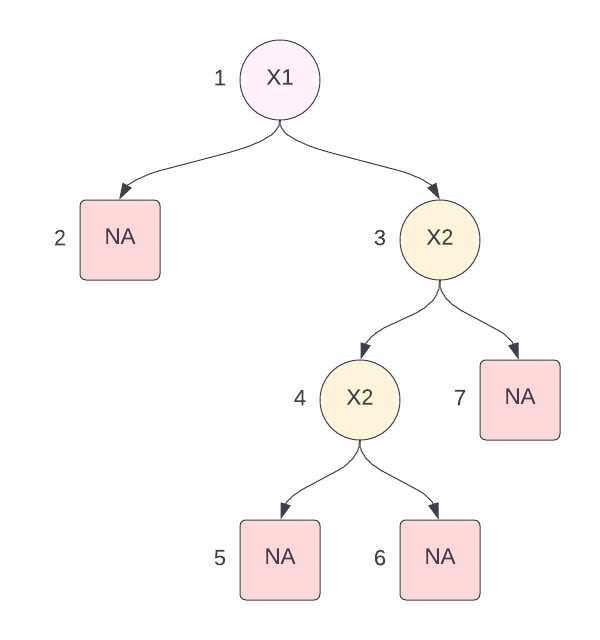
\includegraphics[width=0.6\linewidth]{https://github.com/AlanInglis/bartMan/blob/master/bartman_vignettte_new_plots_1/tree_example.png?raw=true} \end{center}

\protect\hypertarget{fig1:fig1}{}{Figure 1: } Example tree with the
nodes numbered in a depth-first left-side traversal manner.

\hypertarget{visualisations}{%
\section{Visualisations}\label{visualisations}}

\hypertarget{vivi-vsup}{%
\subsection{VIVI-VSUP}\label{vivi-vsup}}

In Inglis et al.~(2022)\footnote{Inglis, A., Parnell, A., \& Hurley, C.
  B. (2022). Visualizing Variable Importance and Variable Interaction
  Effects in Machine Learning Models. Journal of Computational and
  Graphical Statistics, 1-13.}, the authors propose using a heatmap to
display both variable importance (VImp) and variable interactions (VInt)
simultaneously (together VIVI), where the importance values are on the
diagonal and interaction values on the off-diagonal. We adapt the
heatmap displays of importance and interactions to include the
uncertainty by use of a VSUP. To begin we fist generate a heatmap
containing the raw VIVI values without uncertainty.

\begin{Shaded}
\begin{Highlighting}[]
\NormalTok{stdMat }\OtherTok{\textless{}{-}} \FunctionTok{viviBartMatrix}\NormalTok{(trees\_data,}
                          \AttributeTok{type =} \StringTok{\textquotesingle{}standard\textquotesingle{}}\NormalTok{,}
                          \AttributeTok{metric =} \StringTok{\textquotesingle{}propMean\textquotesingle{}}\NormalTok{)}
\end{Highlighting}
\end{Shaded}

Now we create a list of two matrices. One containing the raw inclusion
proportions and one containing the uncertainties. Here we use the
coefficient of variation as our uncertainty measure. However the
standard deviation or standard error is also available by setting
\texttt{metricError\ =\ \textquotesingle{}SD\textquotesingle{}} or
\texttt{metricError\ =\ \textquotesingle{}SE\textquotesingle{}}, in the
code below.

\begin{Shaded}
\begin{Highlighting}[]
\NormalTok{vsupMat }\OtherTok{\textless{}{-}} \FunctionTok{viviBartMatrix}\NormalTok{(trees\_data,}
                          \AttributeTok{type =} \StringTok{\textquotesingle{}vsup\textquotesingle{}}\NormalTok{,}
                          \AttributeTok{metric =} \StringTok{\textquotesingle{}propMean\textquotesingle{}}\NormalTok{,}
                          \AttributeTok{metricError =} \StringTok{"CV"}\NormalTok{)}
\end{Highlighting}
\end{Shaded}

Once the matrices have been created, they can be plotted displaying a
VSUP plot with the uncertainty included. For illustration purposes only
we show the plot without uncertainty in Figure 1 and with uncertainty in
Figure 2:

\begin{Shaded}
\begin{Highlighting}[]
\FunctionTok{viviBartPlot}\NormalTok{(stdMat)}
\end{Highlighting}
\end{Shaded}

\begin{center}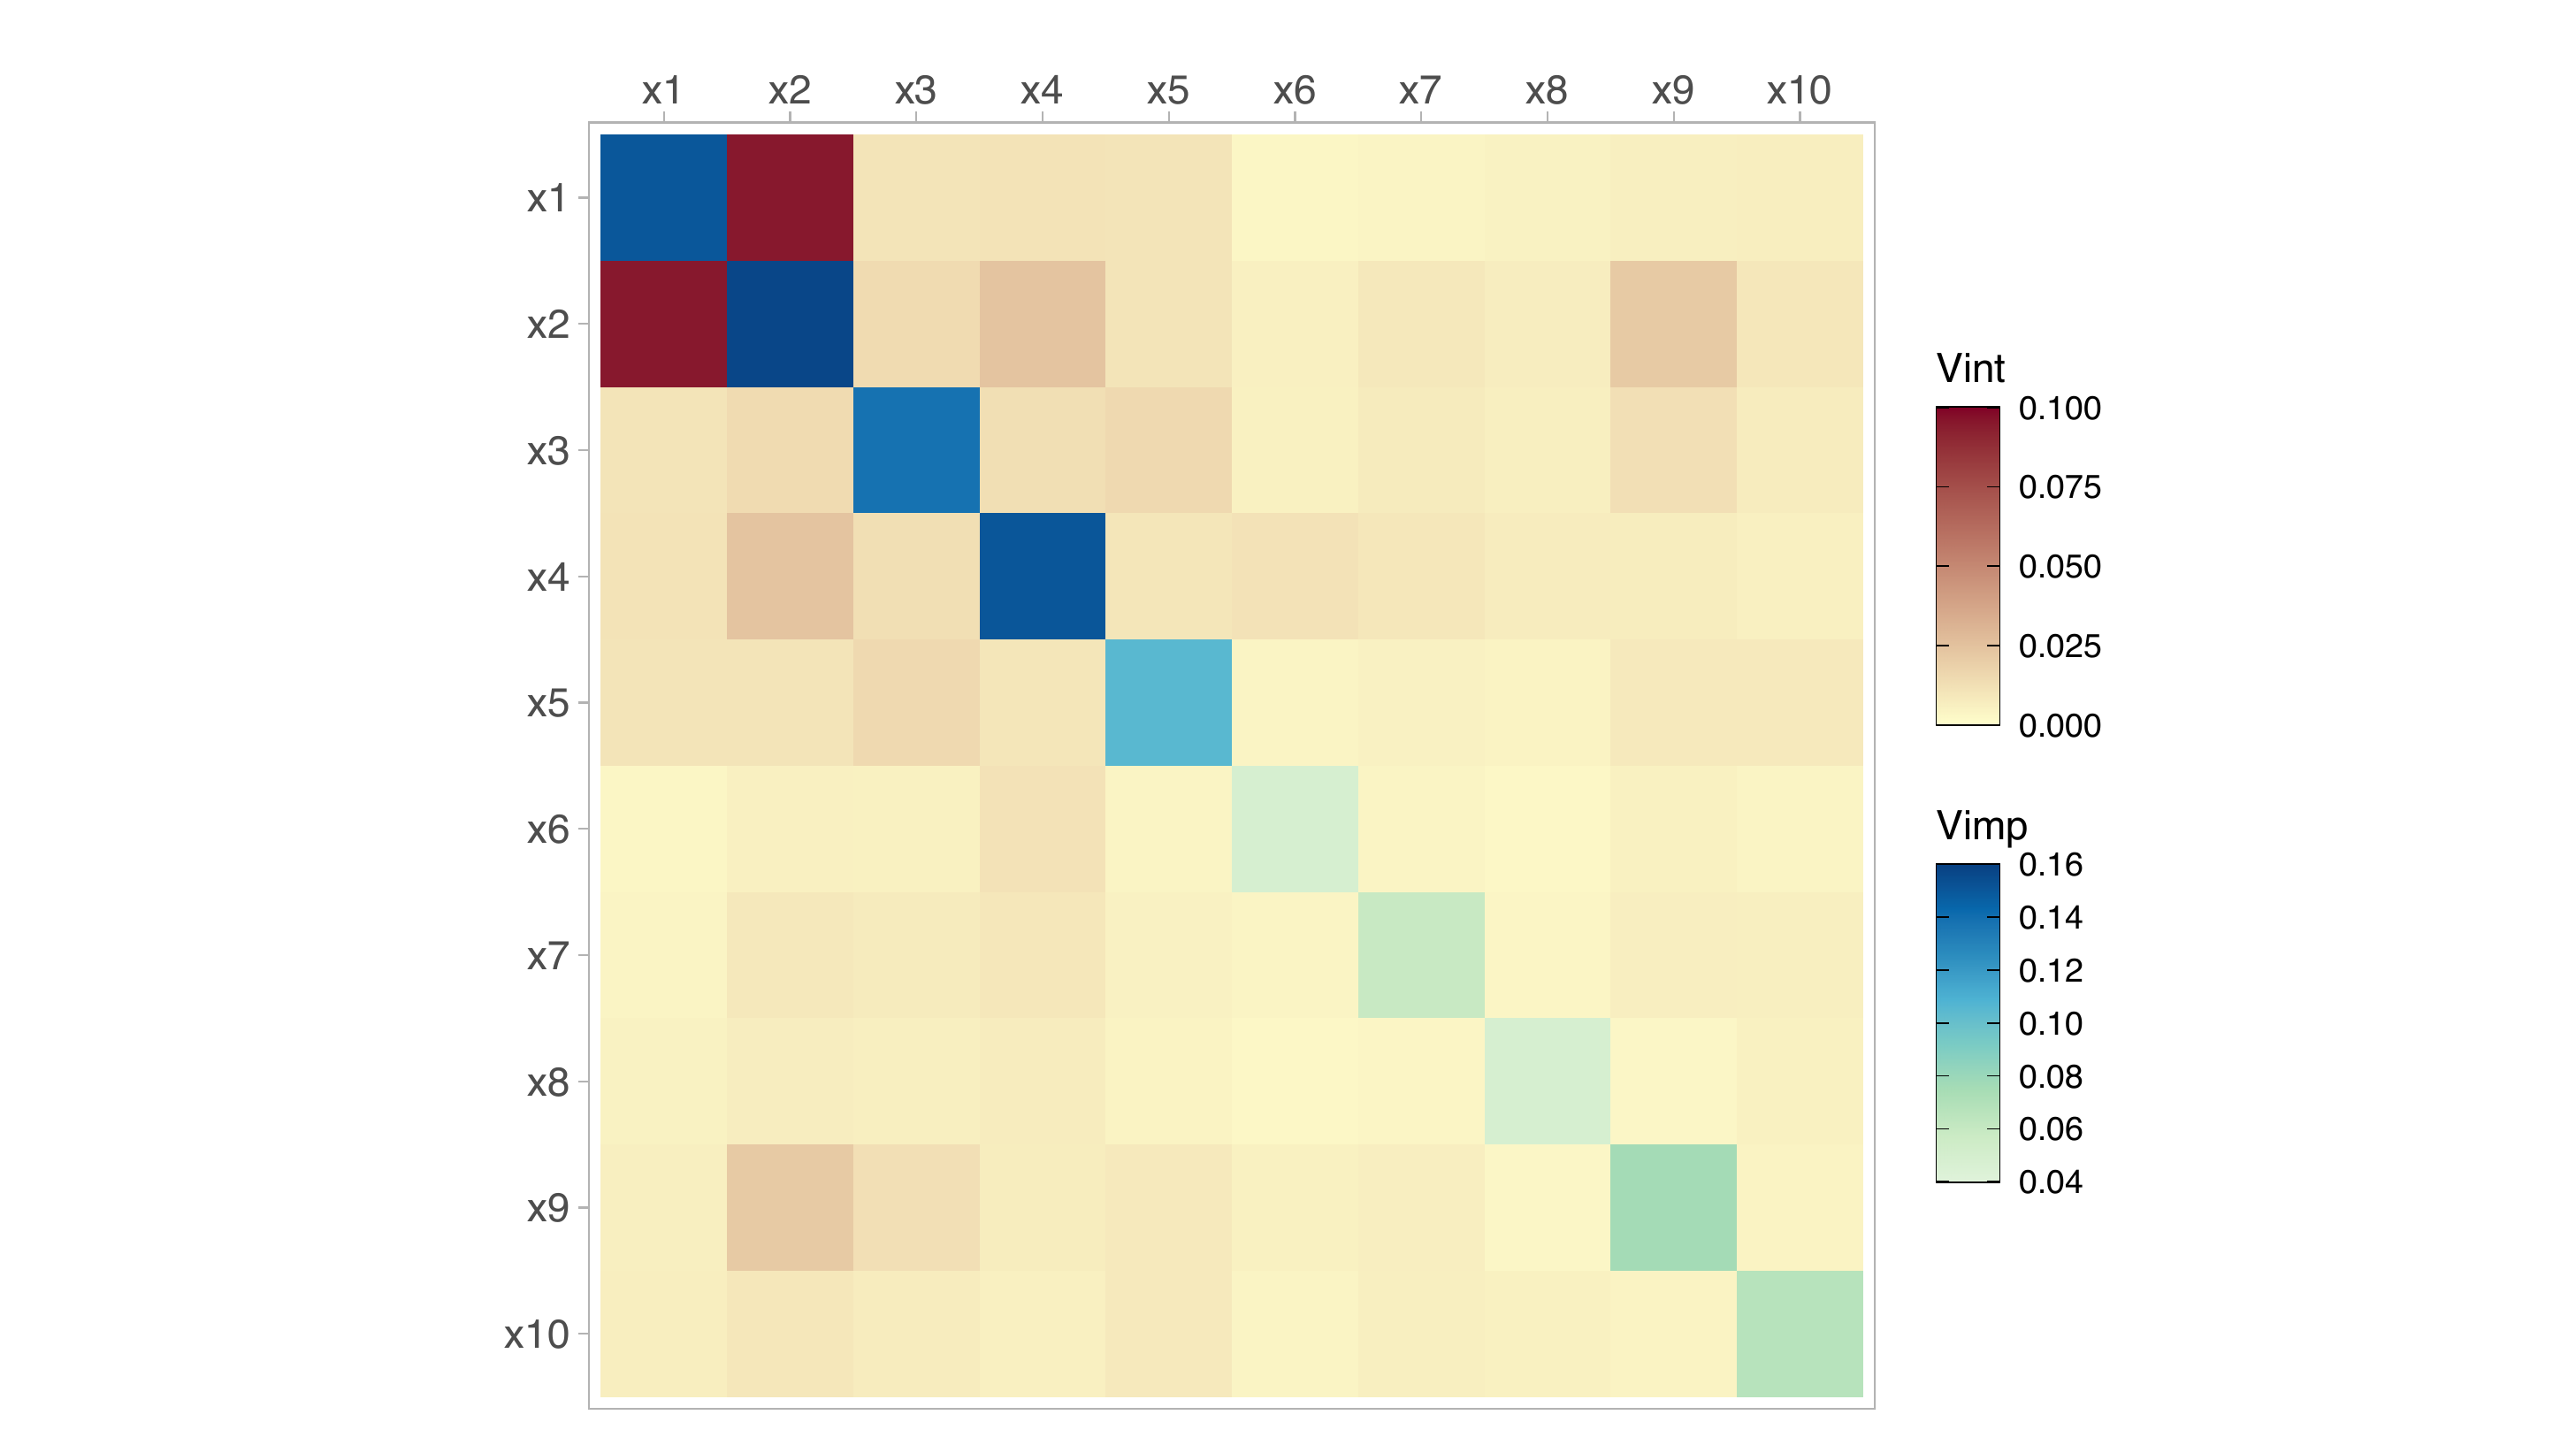
\includegraphics[width=1\linewidth]{https://github.com/AlanInglis/bartMan/blob/master/bartman_vignettte_new_plots_1/heatmap_vivid_1.png?raw=true} \end{center}

\protect\hypertarget{fig2:fig2}{}{Figure 2: } Variable importance and
interaction plot without uncertainty. The interaction between \(x_1\)
and \(x_2\) is clear. The five important variables (\(x_1\) to \(x_5\))
are highlighted. We can also see spurious importance and interaction
values among the noise variables.

\begin{Shaded}
\begin{Highlighting}[]
\FunctionTok{viviBartPlot}\NormalTok{(vsupMat,}
             \AttributeTok{max\_desat =} \DecValTok{1}\NormalTok{,}
             \AttributeTok{pow\_desat =} \FloatTok{0.6}\NormalTok{,}
             \AttributeTok{max\_light =} \FloatTok{0.6}\NormalTok{,}
             \AttributeTok{pow\_light =} \DecValTok{1}\NormalTok{,}
             \AttributeTok{label =} \StringTok{\textquotesingle{}CV\textquotesingle{}}\NormalTok{)}
\end{Highlighting}
\end{Shaded}

\begin{center}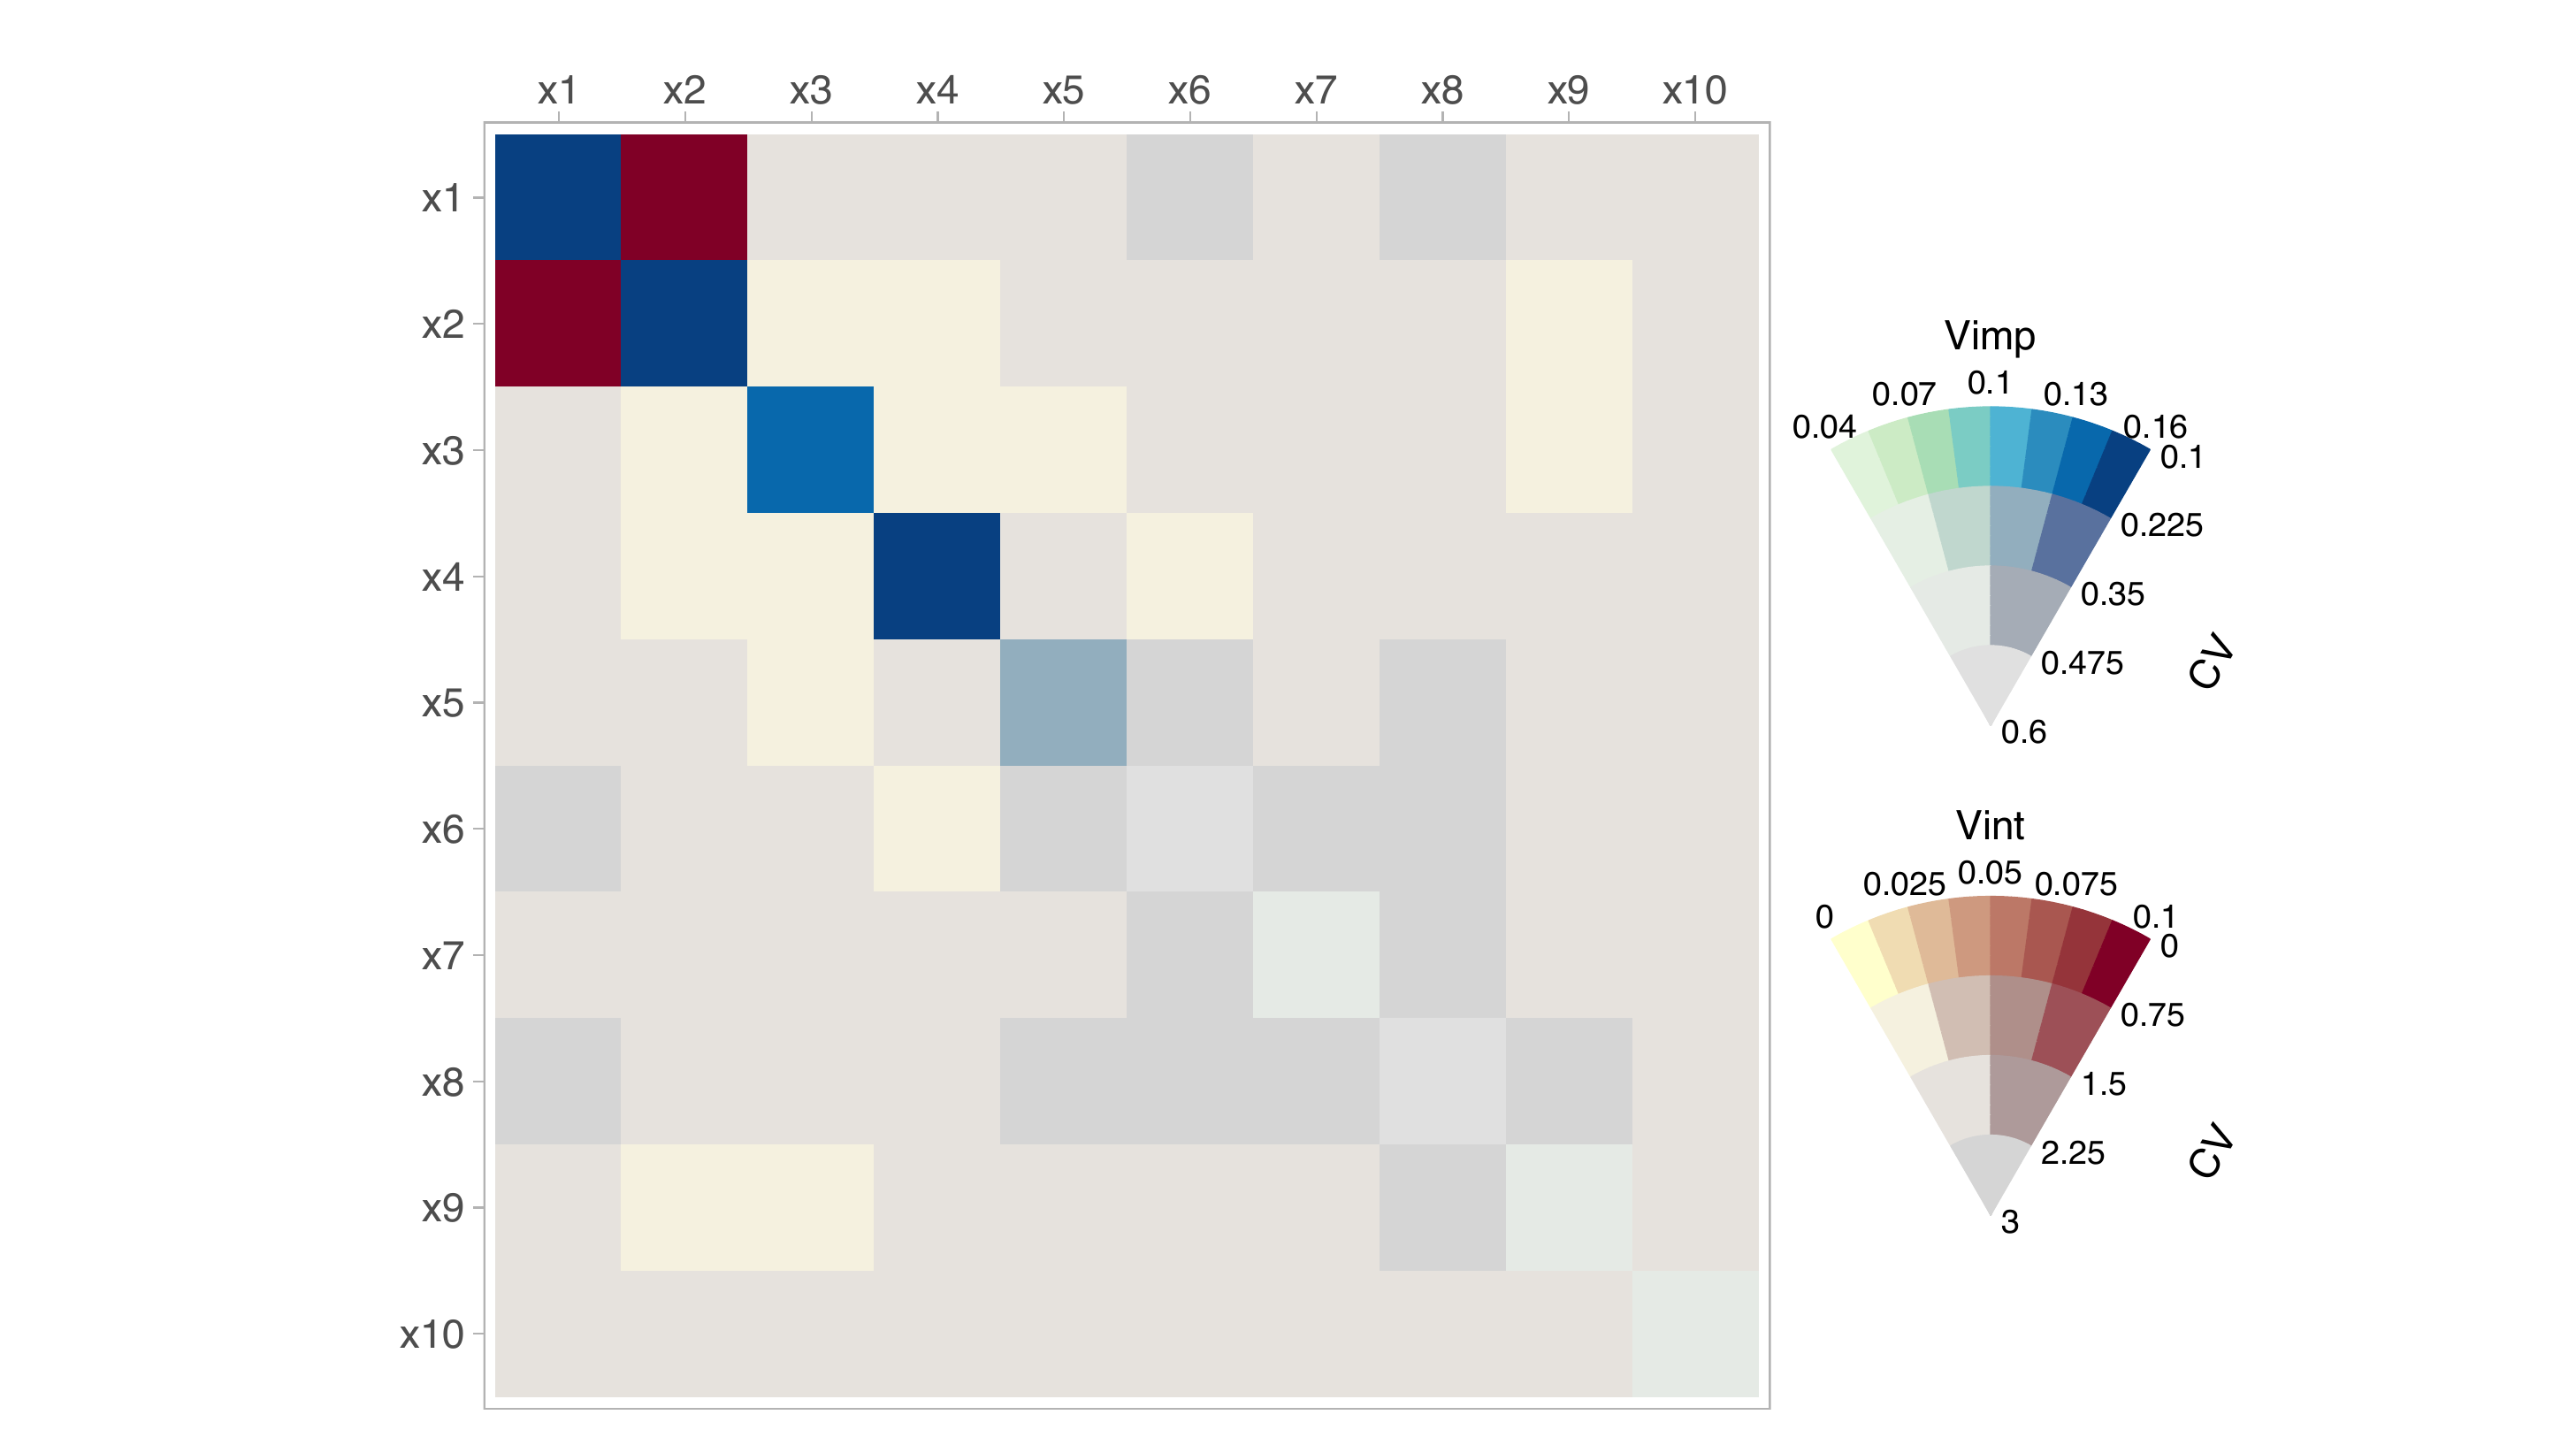
\includegraphics[width=1\linewidth]{https://github.com/AlanInglis/bartMan/blob/master/bartman_vignettte_new_plots_1/heatmap_vsup_1.png?raw=true} \end{center}

\protect\hypertarget{fig3:fig3}{}{Figure 3: } Variable importance and
interaction plot with uncertainty. We can see that the interaction
values for the noise variables have a high coefficient of variation
associated with them..

\hypertarget{tree-based-plots}{%
\subsection{Tree Based Plots}\label{tree-based-plots}}

Here we examine more closely the structure of the decision trees created
when building a BART model. Examining the tree structure may yield
information on the stability and variability of the tree structures as
the algorithm iterates to create the posterior. By sorting and colouring
the trees appropriately we can identify important variables and common
interactions between variables for a given iteration. Alternatively we
can look at how a single tree evolves through the iteration to explore
the fitting algorithm's stability.

To plot an individual tree, we can choose to display it either in
dendrogram format, or icicle format. Additionally, we can choose which
tree number or iteration to display:

\begin{Shaded}
\begin{Highlighting}[]
\FunctionTok{plotSingleTree}\NormalTok{(}\AttributeTok{treeData =}\NormalTok{ trees\_data, }\AttributeTok{treeNo =} \DecValTok{1}\NormalTok{, }\AttributeTok{iter =} \DecValTok{1}\NormalTok{, }\AttributeTok{plotType =} \StringTok{"dendrogram"}\NormalTok{)}
\FunctionTok{plotSingleTree}\NormalTok{(}\AttributeTok{treeData =}\NormalTok{ trees\_data, }\AttributeTok{treeNo =} \DecValTok{1}\NormalTok{, }\AttributeTok{iter =} \DecValTok{1}\NormalTok{, }\AttributeTok{plotType =} \StringTok{"icicle"}\NormalTok{)}
\end{Highlighting}
\end{Shaded}

\begin{center}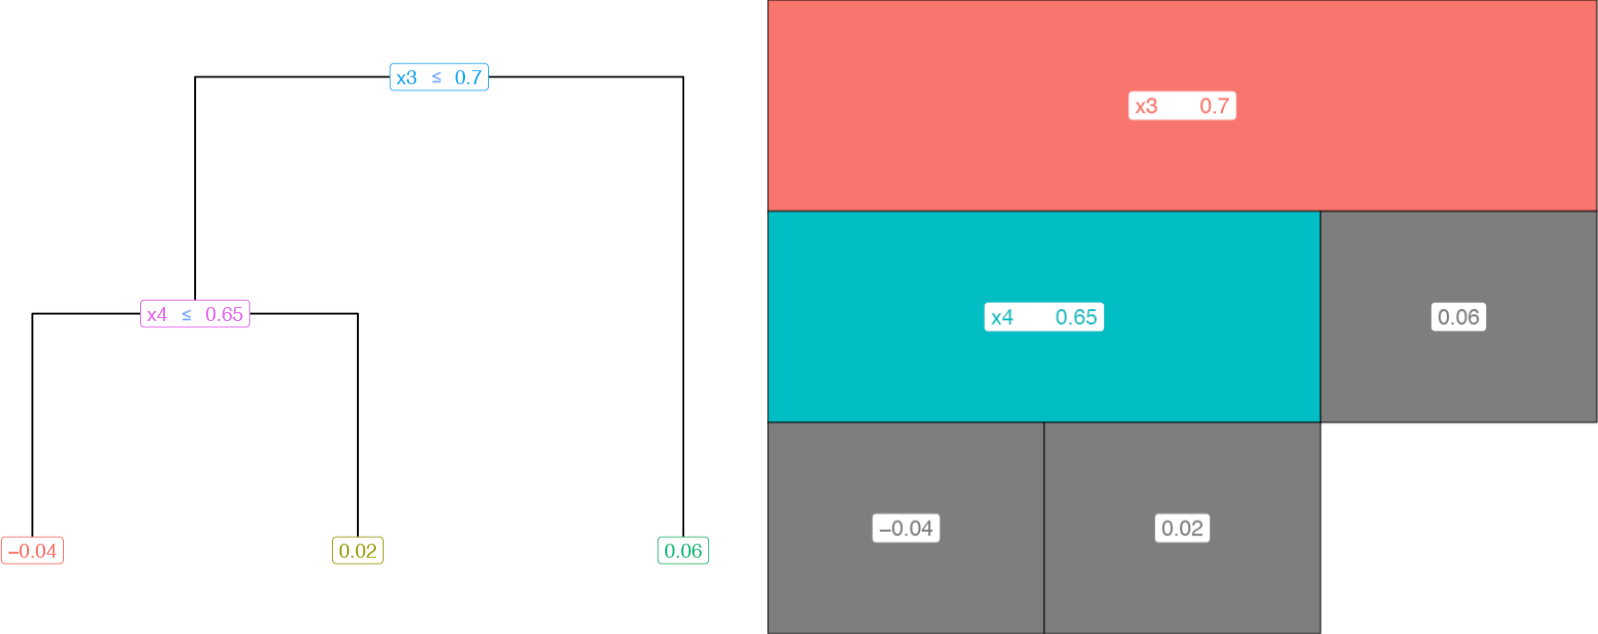
\includegraphics[width=1\linewidth]{https://github.com/AlanInglis/bartMan/blob/master/bartman_vignettte_new_plots_1/single_trees_1.png?raw=true} \end{center}

\protect\hypertarget{fig4:fig4}{}{Figure 4: }A dendrogram plot of a
selected tree (left) and an icicle plot of a selected tree (right). In
the icicle plot, the nodes are colored by the variable used in the
splitting rule. Leaf (terminal) nodes are colored grey.

The \texttt{plotTrees} function allows for a few different options when
plotting. For example, we can chose to display all the trees from a
selected iteration:

\begin{Shaded}
\begin{Highlighting}[]
\FunctionTok{plotTrees}\NormalTok{(}\AttributeTok{trees =}\NormalTok{ trees\_data, }\AttributeTok{iter =} \DecValTok{1}\NormalTok{)}
\end{Highlighting}
\end{Shaded}

\begin{center}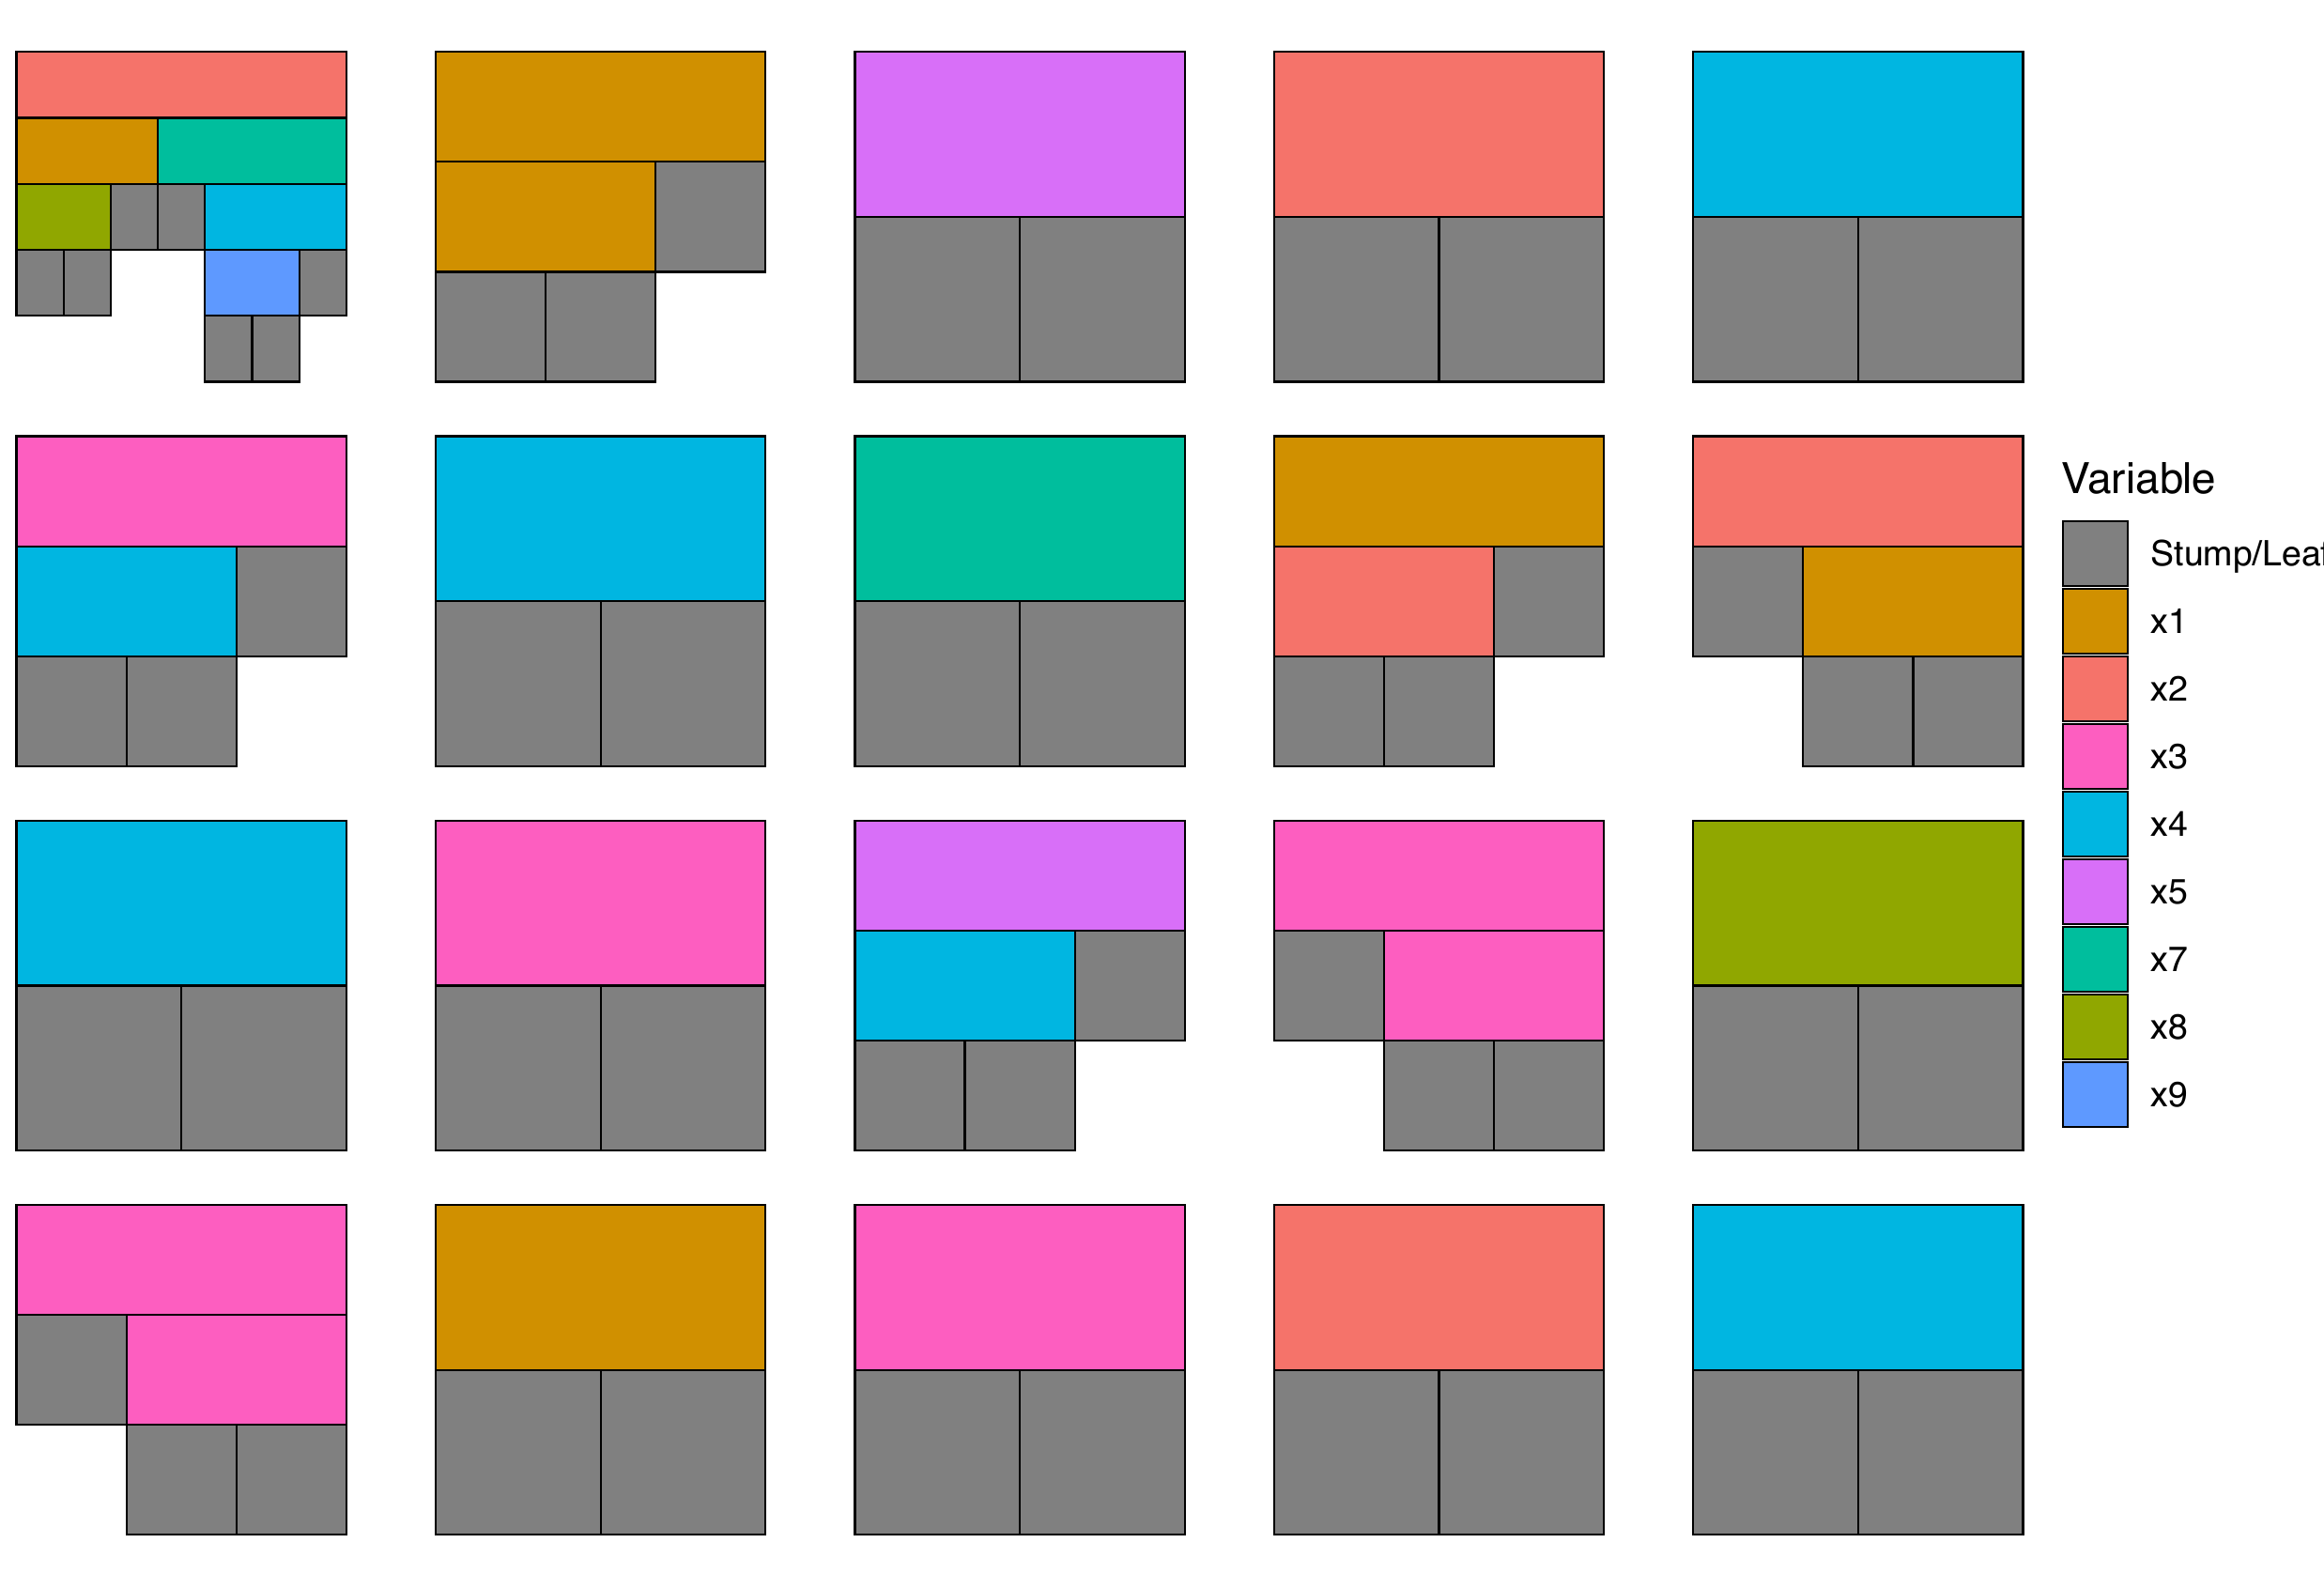
\includegraphics[width=1\linewidth]{https://github.com/AlanInglis/bartMan/blob/master/bartman_vignettte_new_plots_1/trees_iter_1_1.png?raw=true} \end{center}

\protect\hypertarget{fig5:fig5}{}{Figure 5: }All trees from a single
iteration. In this case the first iteration is shown.

The function arguments for \texttt{plotTrees} are outlined as follows:

• \texttt{trees}: A data frame of trees, usually created via
\texttt{extractTreeData()}.

• \texttt{iter}: An integer specifying the iteration number of trees to
be included in the output. If NULL, trees from all iterations are
included.

• \texttt{treeNo}: An integer specifying the number of the tree to
include in the output. If NULL, all trees are included.

• \texttt{fillBy}: A character string specifying the attribute to color
nodes by. Options are `response' for coloring nodes based on their mean
response values or `mu' for coloring nodes based on their predicted
value, or NULL for no specific fill attribute.

• \texttt{sizeNodes} A logical value indicating whether to adjust node
sizes. If TRUE, node sizes are adjusted; if FALSE, all nodes are given
the same size.

• \texttt{removeStump} A logical value. If TRUE, then stumps are removed
from plot.

• \texttt{selectedVars} A vector of selected variables to display.
Either a character vector of names or the variables column number.

• \texttt{pal} A colour palette for node colouring. Palette is used when
`fillBy' is specified for gradient colouring.

• \texttt{center\_Mu} A logical value indicating whether to center the
color scale for the `mu' attribute around zero. Applicable only when
`fillBy' is set to ``mu''.

• \texttt{cluster} A character string that specifies the criterion for
reordering trees in the output. Currently supports ``depth'' for
ordering by the maximum depth of nodes, and ``var'' for a clustering
based on variables. If NULL, no reordering is performed.

When the number of variables or trees is large it can become harder to
identify interesting features. We provide a plot that can be used to
highlight interesting features by accentuating selected variables by
coloring them brightly while uniformly coloring the remaining variables
a light grey. We can then couple this with a sorting step to order the
trees by the most frequent tree structure.

\begin{Shaded}
\begin{Highlighting}[]
\FunctionTok{plotTrees}\NormalTok{(}\AttributeTok{trees =}\NormalTok{ trees\_data,}
          \AttributeTok{iter =} \DecValTok{1}\NormalTok{,}
          \AttributeTok{removeStump =} \ConstantTok{TRUE}\NormalTok{,}
          \AttributeTok{selectedVars =} \FunctionTok{c}\NormalTok{(}\StringTok{\textquotesingle{}x4\textquotesingle{}}\NormalTok{),}\CommentTok{\#c(\textquotesingle{}x1\textquotesingle{},\textquotesingle{}x2\textquotesingle{},\textquotesingle{}x3\textquotesingle{},\textquotesingle{}x4\textquotesingle{},\textquotesingle{}x5\textquotesingle{}),}
          \AttributeTok{cluster =} \StringTok{\textquotesingle{}var\textquotesingle{}}\NormalTok{)}
\end{Highlighting}
\end{Shaded}

\begin{center}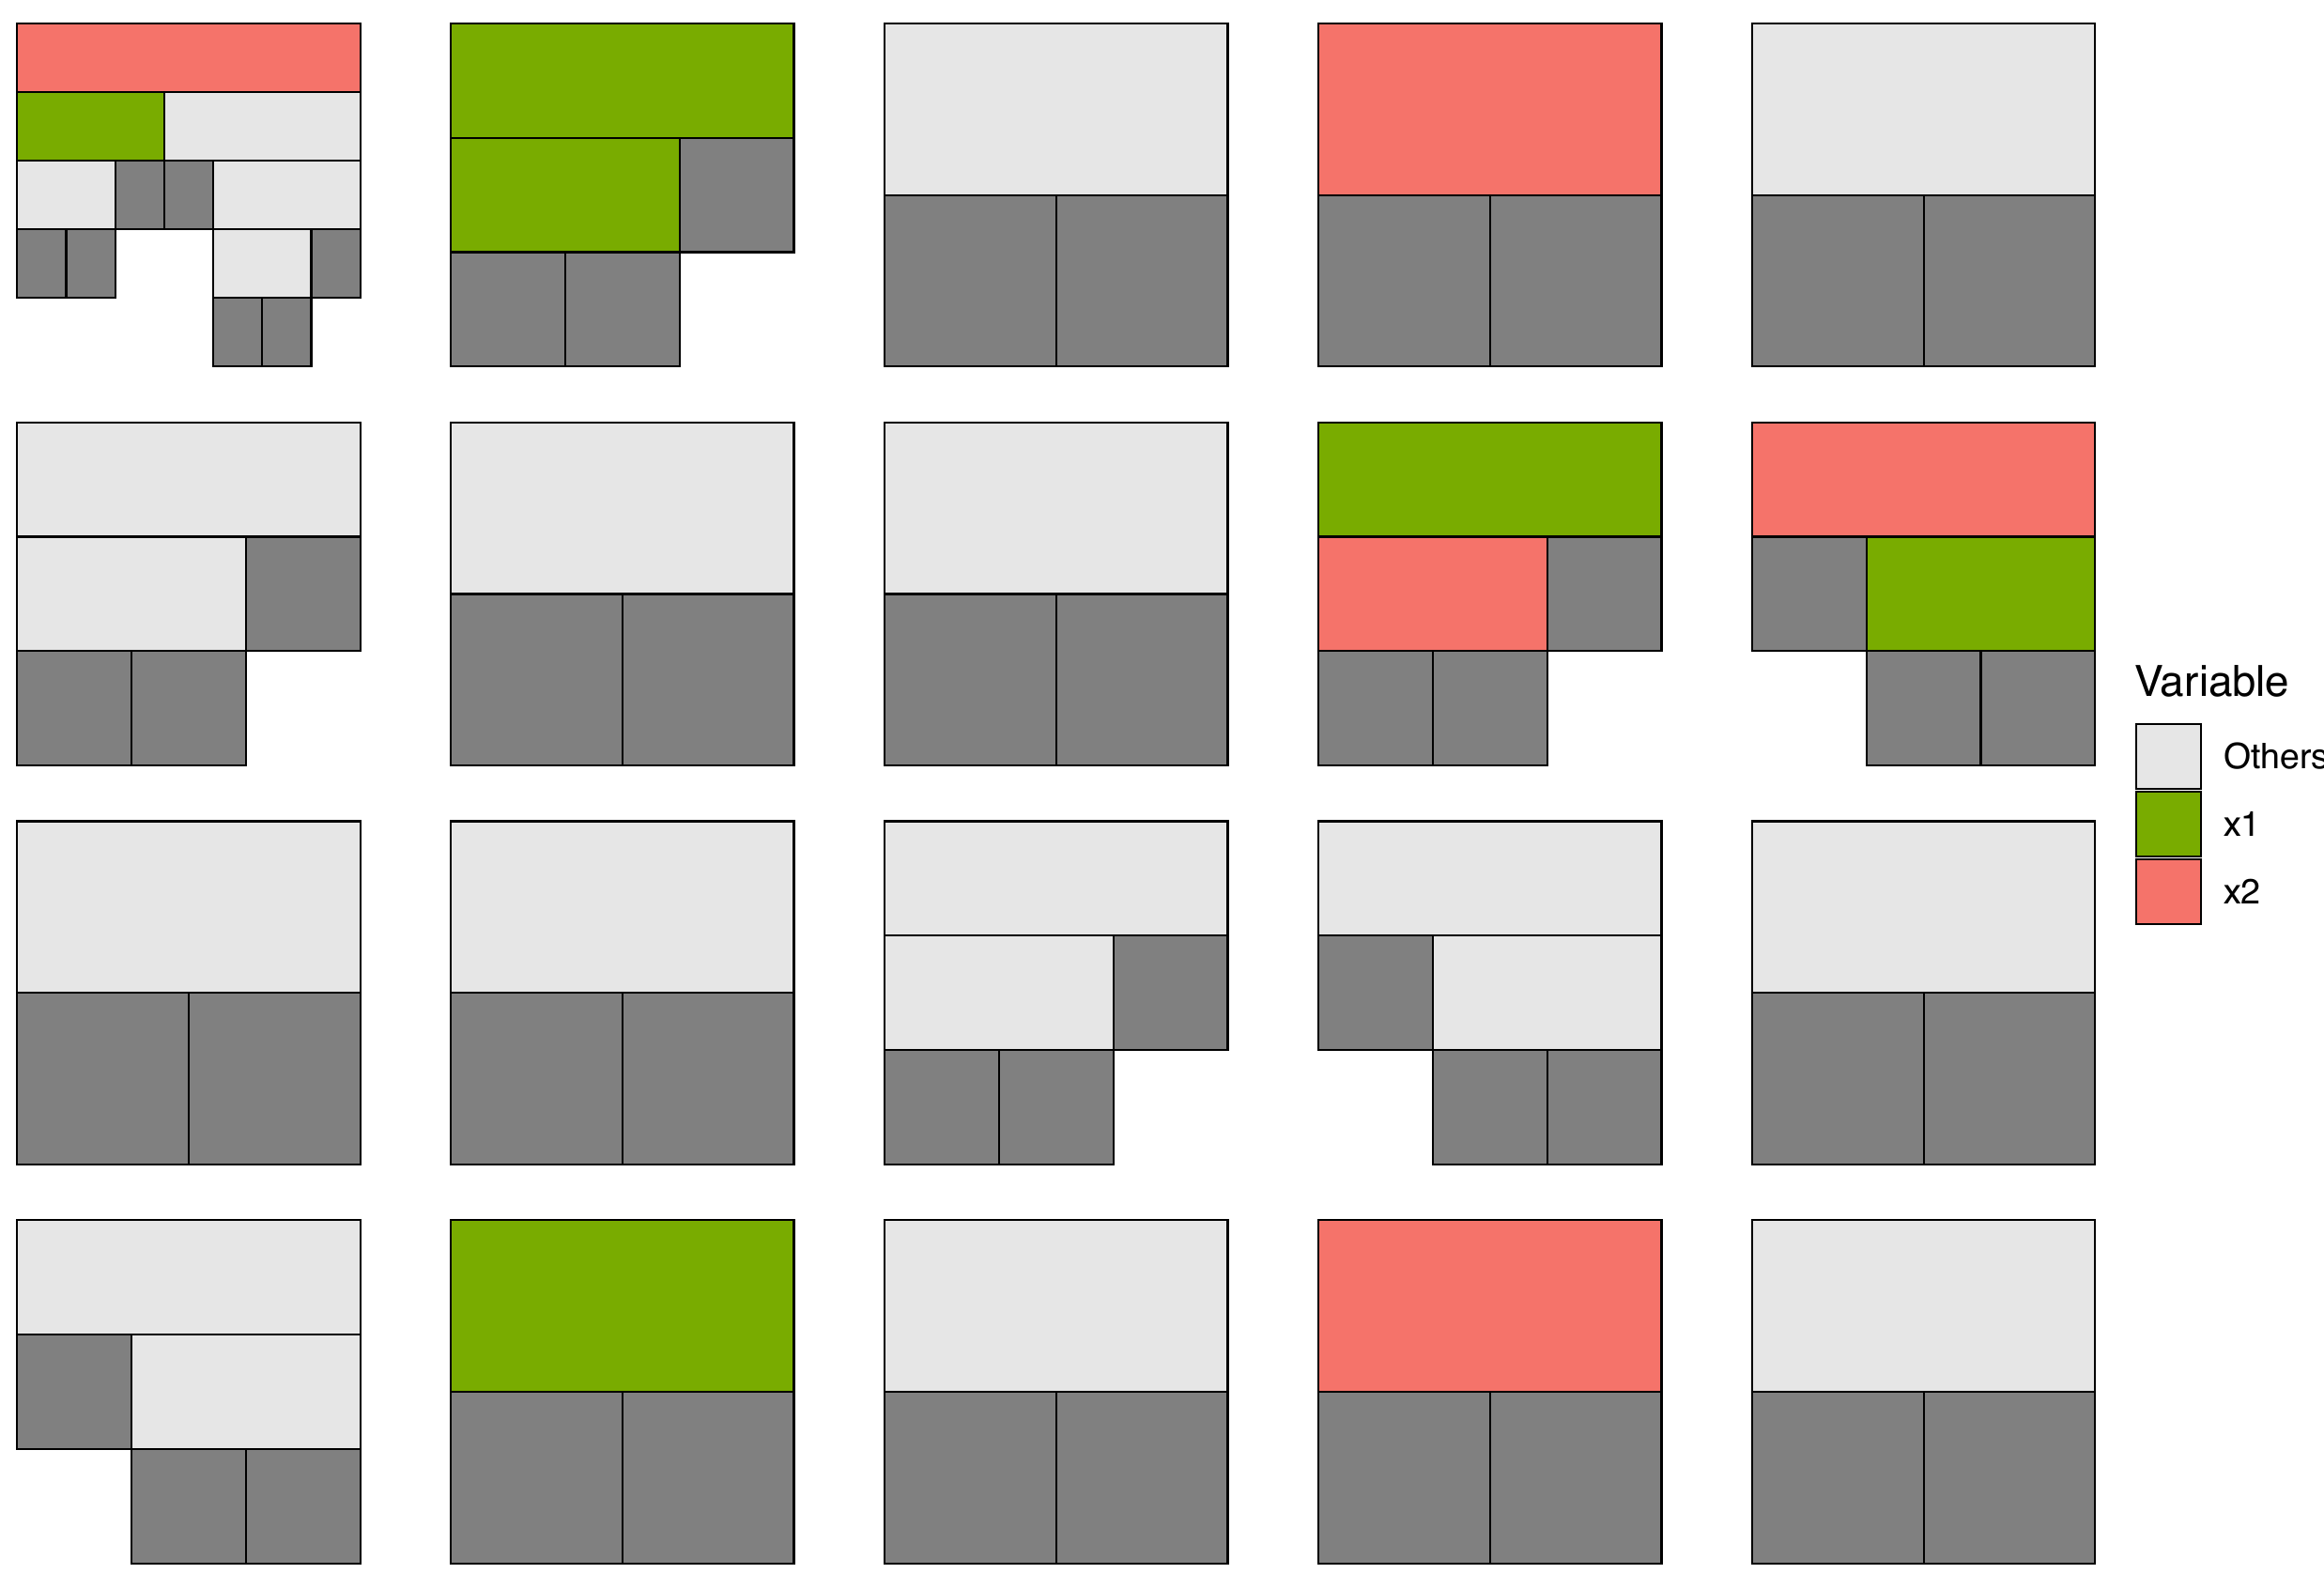
\includegraphics[width=1\linewidth]{https://github.com/AlanInglis/bartMan/blob/master/bartman_vignettte_new_plots_1/trees_selected_1.png?raw=true} \end{center}

\protect\hypertarget{fig6:fig6}{}{Figure 6: }All trees from a single
iteration. In this case the first iteration is shown, the stumps have
been removed, and the trees have been sorted according to their
structure.

Additionally, we can plot a single tree over all iterations by selecting
a tree vis the \texttt{treeNo} argument. This shows us visually BART's
\emph{grow, prune, change, swap} mechanisms in action.

\begin{Shaded}
\begin{Highlighting}[]
\FunctionTok{plotTrees}\NormalTok{(}\AttributeTok{trees =}\NormalTok{ trees\_data, }\AttributeTok{treeNo =} \DecValTok{1}\NormalTok{)}
\end{Highlighting}
\end{Shaded}

\begin{center}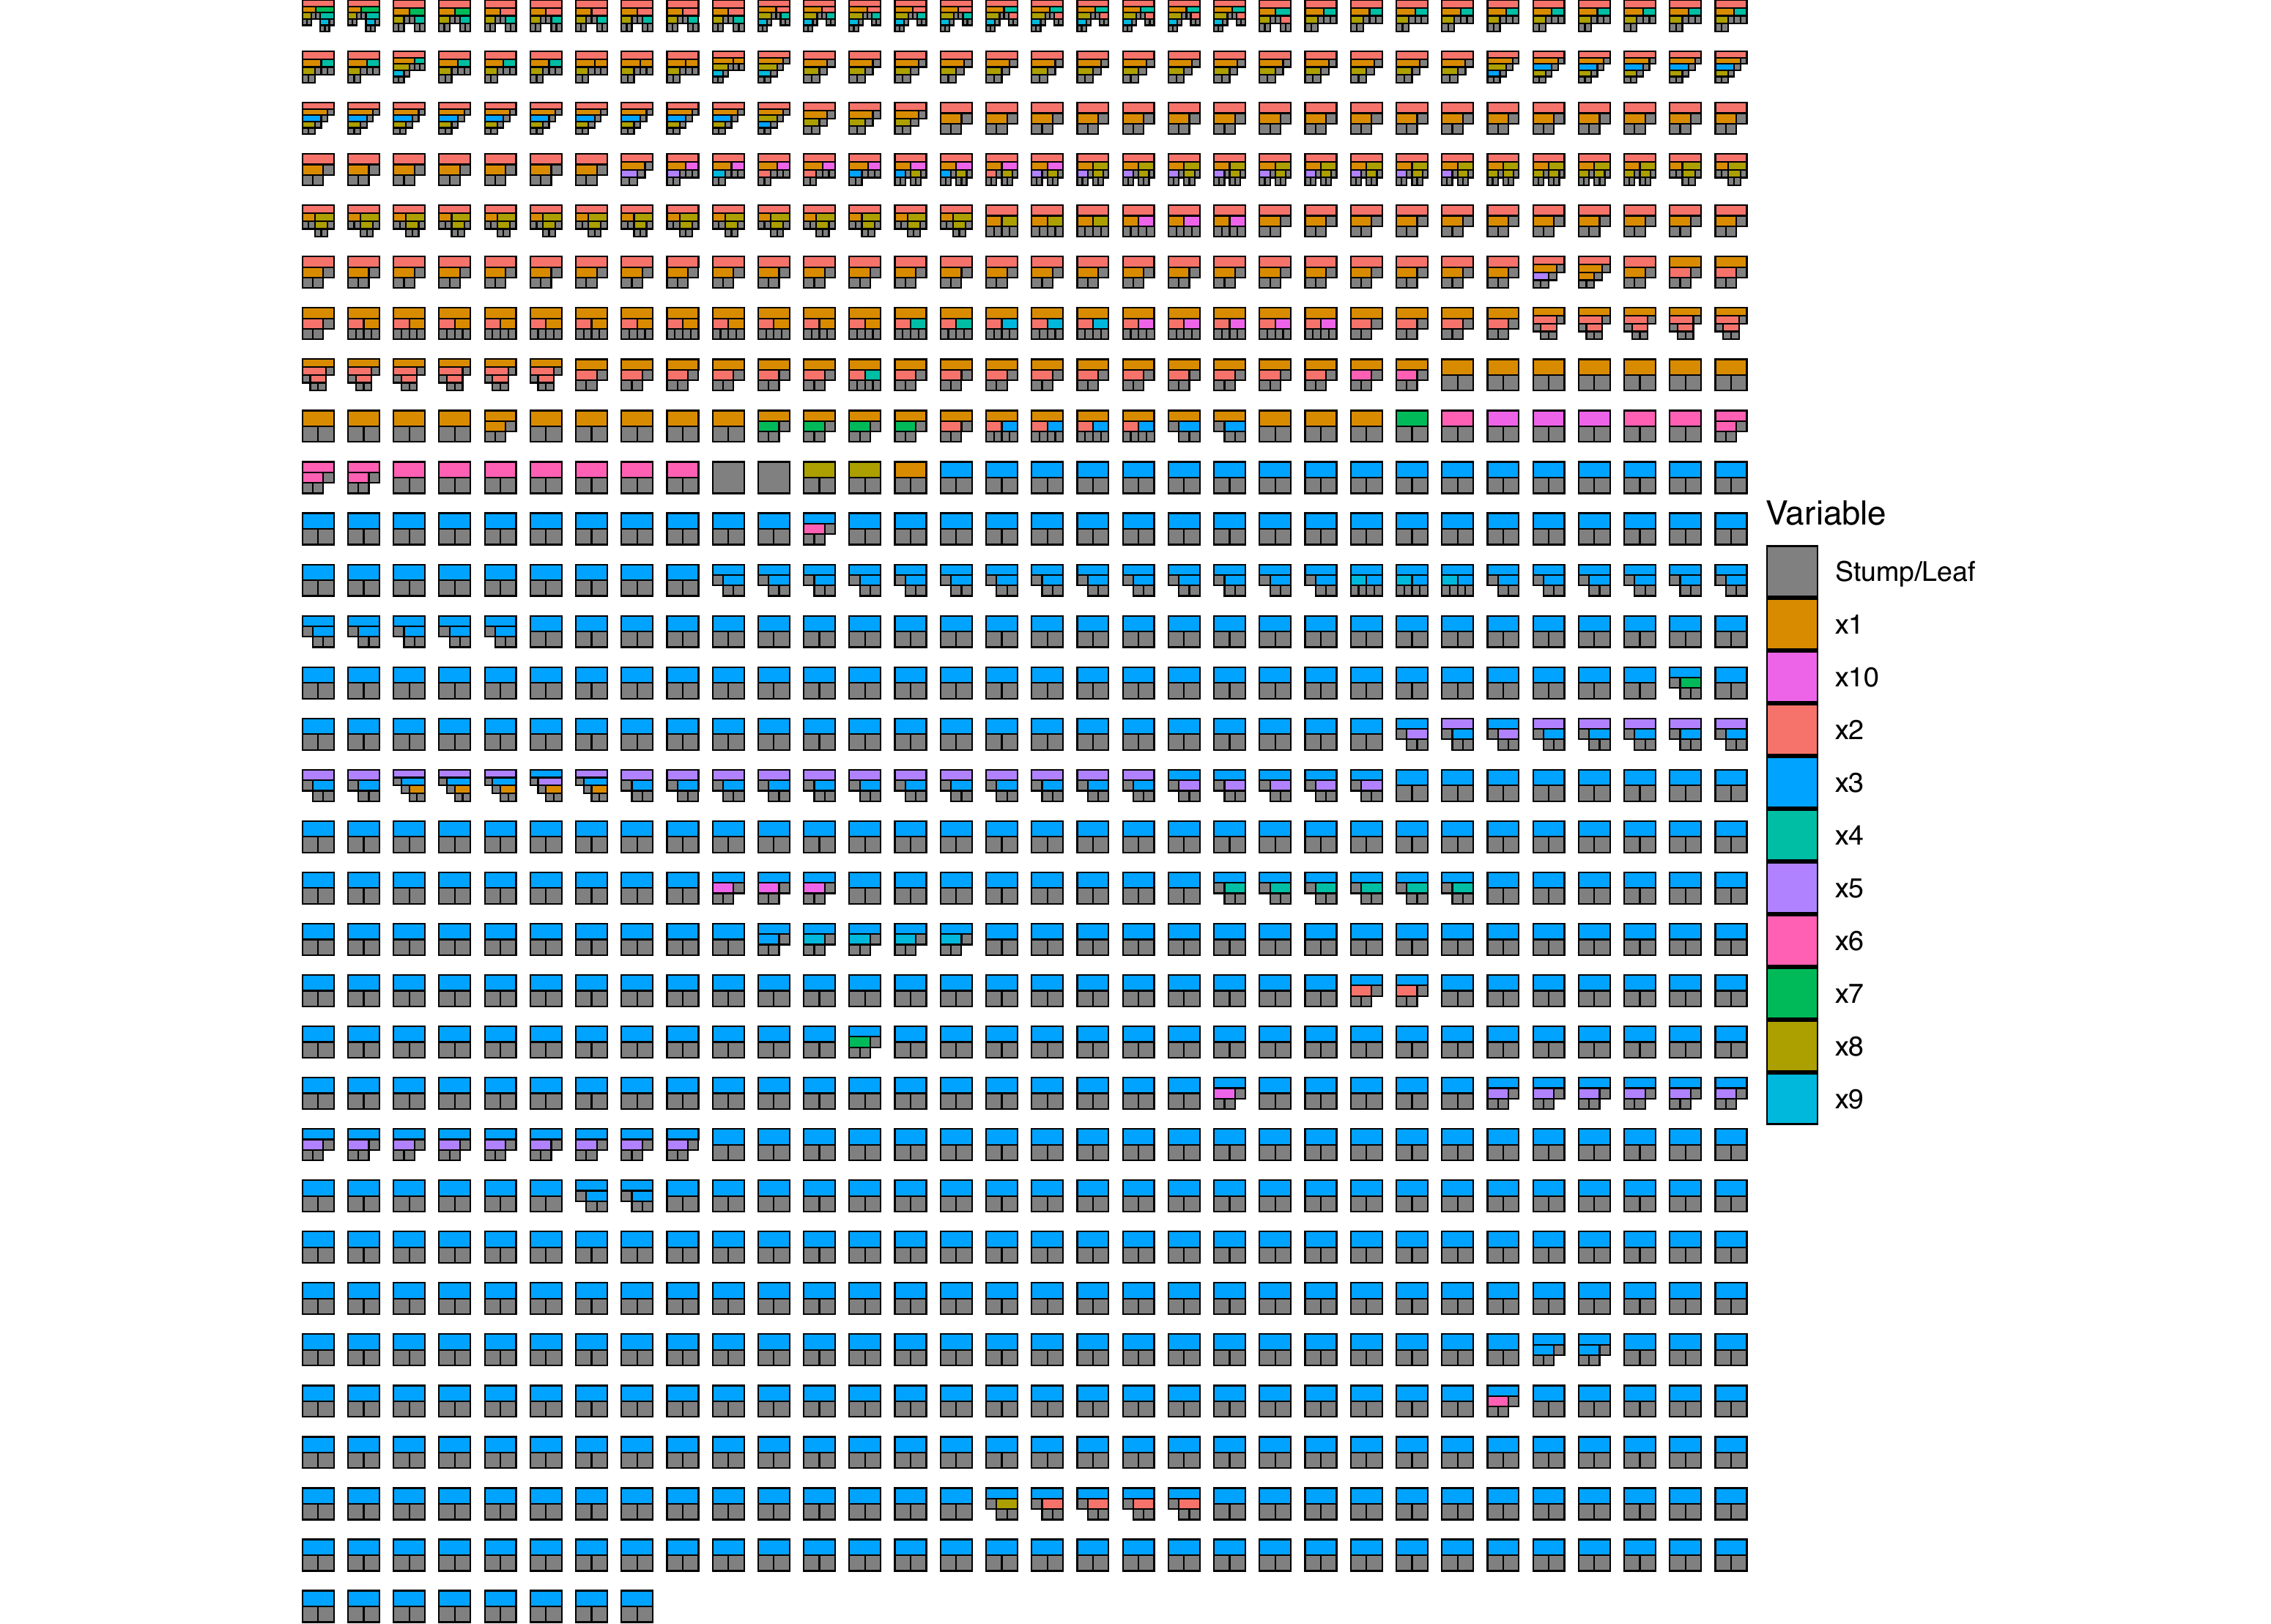
\includegraphics[width=1\linewidth]{https://github.com/AlanInglis/bartMan/blob/master/bartman_vignettte_new_plots_1/trees_treeNum_1_1.png?raw=true} \end{center}

\protect\hypertarget{fig7:fig7}{}{Figure 7: }A single tree over all
iterations.

When viewing the trees, it can be useful to view different aspects or
metrics. In Figure 7 we show some of these aspects by displaying all the
trees in a selected iteration. For example, in (a) we color terminal
nodes and stumps by the mean response. In (b) we color them by the
terminal node parameter value. In (c) we sort the trees by structure
starting with the most common tree and descending to the least common
tree found (useful for identifying the most important splits). Finally,
in (d) we sort the trees by depth. As the \(\mu\) values in (b) are
centered around zero, we use a single-hue, colorblind friendly,
diverging color palette to display the values. For comparison, we use
the same palette to represent the mean response values in (a).

\begin{Shaded}
\begin{Highlighting}[]
\FunctionTok{plotTrees}\NormalTok{(}\AttributeTok{trees =}\NormalTok{ trees\_data, }\AttributeTok{iter =} \DecValTok{1}\NormalTok{, }\AttributeTok{sizeNode =}\NormalTok{ T, }\AttributeTok{fillBy =} \StringTok{\textquotesingle{}mu\textquotesingle{}}\NormalTok{)}
\FunctionTok{plotTrees}\NormalTok{(}\AttributeTok{trees =}\NormalTok{ trees\_data, }\AttributeTok{iter =} \DecValTok{1}\NormalTok{, }\AttributeTok{sizeNode =}\NormalTok{ T, }\AttributeTok{fillBy =} \StringTok{\textquotesingle{}response\textquotesingle{}}\NormalTok{)}
\FunctionTok{plotTrees}\NormalTok{(}\AttributeTok{trees =}\NormalTok{ trees\_data, }\AttributeTok{iter =} \DecValTok{1}\NormalTok{, }\AttributeTok{cluster =} \StringTok{"depth"}\NormalTok{)}
\FunctionTok{plotTrees}\NormalTok{(}\AttributeTok{trees =}\NormalTok{ trees\_data, }\AttributeTok{iter =} \DecValTok{1}\NormalTok{, }\AttributeTok{cluster =} \StringTok{"var"}\NormalTok{)}
\end{Highlighting}
\end{Shaded}

\begin{center}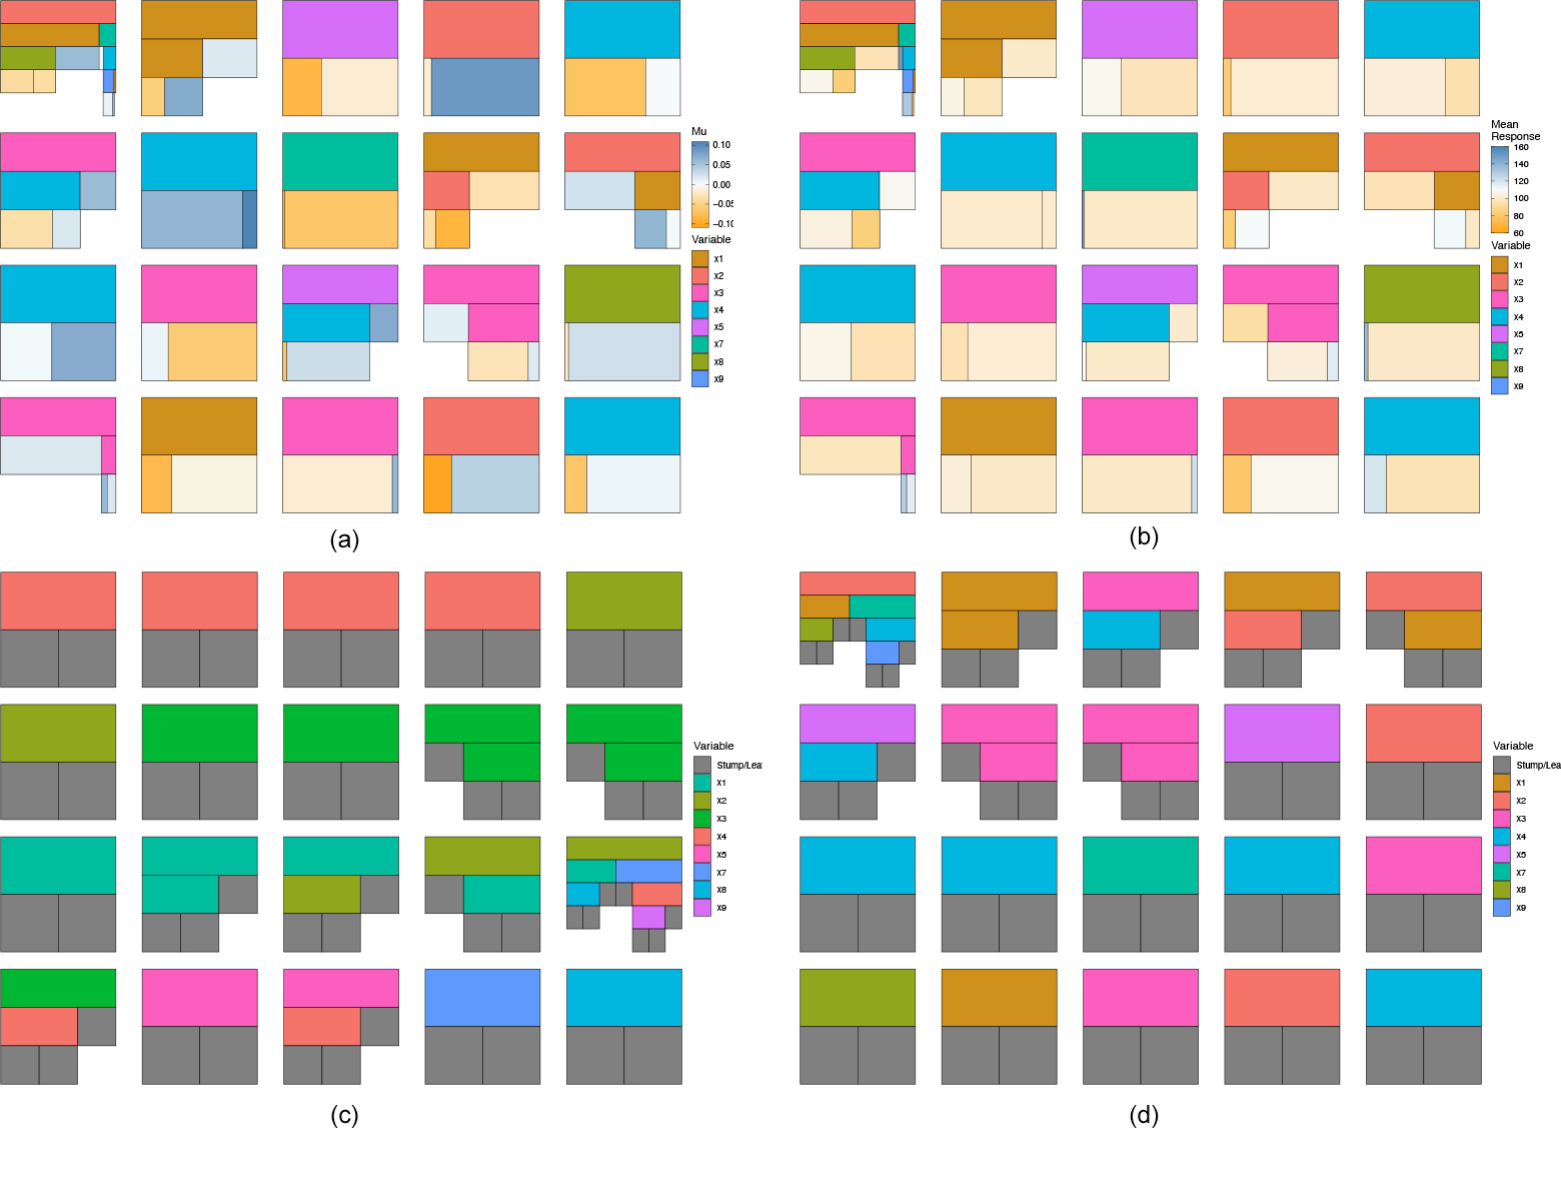
\includegraphics[width=1\linewidth]{https://github.com/AlanInglis/bartMan/blob/master/bartman_vignettte_new_plots_1/tree_quad_1.png?raw=true} \end{center}

\protect\hypertarget{fig8:fig8}{}{Figure 8: }All trees in a selected
iteration. In (a) the terminal nodes and stumps are colored by the mean
response. In (b) the terminal nodes and stumps are colored by the
predicted value \(\mu\). In (c) we sort the trees by structure starting
with the most common tree and descending to the least common tree shape
and in (d) we sort the trees by tree depth.

As an alternative to the sorting of the tree structures, seen in Figure
7 (c), we provide a bar plot summarizing the tree structures. Here we
choose to display the top 10 most frequent tree structures, however
displaying a single tree across iterations or displaying all trees in a
single iteration is possible via the \texttt{iter} and \texttt{treeNo}
arguments.

\begin{Shaded}
\begin{Highlighting}[]
\FunctionTok{treeBarPlot}\NormalTok{(}\AttributeTok{trees =}\NormalTok{ trees\_data, }\AttributeTok{topTrees =} \DecValTok{10}\NormalTok{, }\AttributeTok{iter =} \ConstantTok{NULL}\NormalTok{)}
\end{Highlighting}
\end{Shaded}

\begin{center}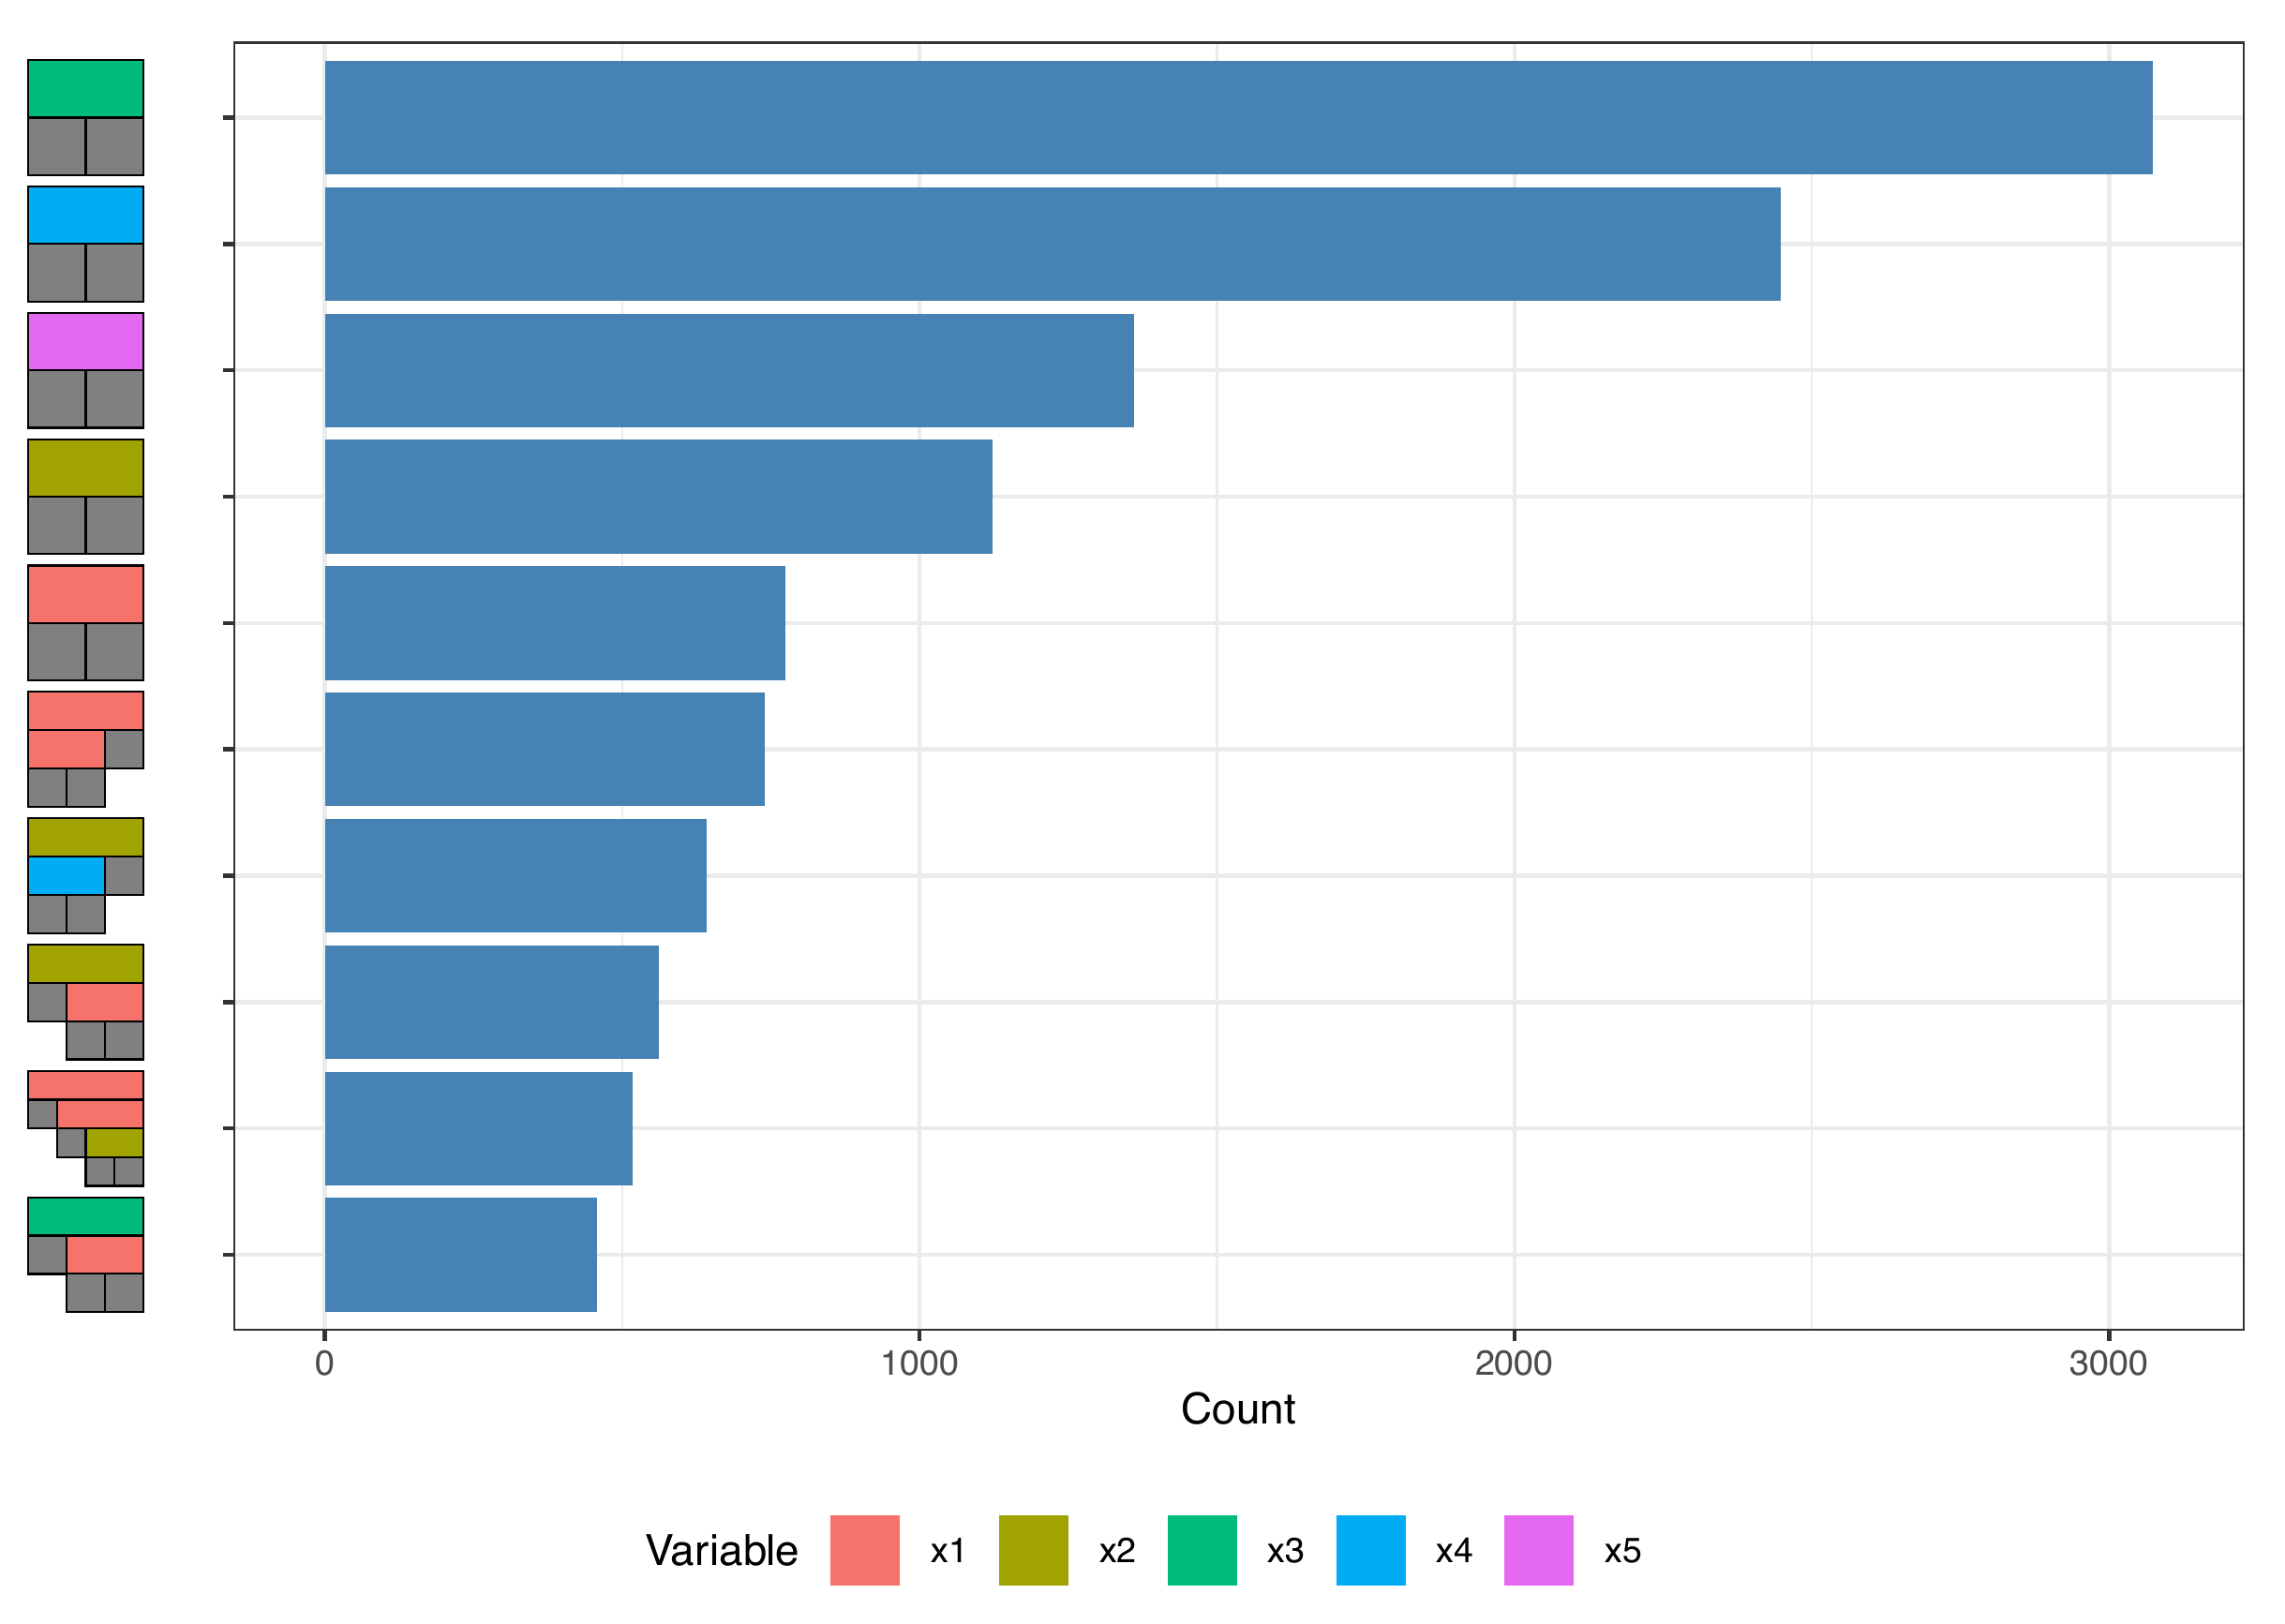
\includegraphics[width=0.8\linewidth]{https://github.com/AlanInglis/bartMan/blob/master/bartman_vignettte_new_plots_1/trees_barplot_1.png?raw=true} \end{center}

\protect\hypertarget{fig9:fig9}{}{Figure 9: } Bar plot of the top 10
most frequent tree types over all iterations. Trees with a single binary
split on Petal.Length occur the most often.

\hypertarget{proximity-matrix-and-multidimensional-scaling}{%
\subsection{Proximity Matrix and Multidimensional
Scaling}\label{proximity-matrix-and-multidimensional-scaling}}

Proximity matrices combined with multidimensional scaling (MDS) are
commonly used in random forests to identify outlying
observations\footnote{Breiman, L. (2001). Random forests. Machine
  learning, 45(1), 5-32.Chicago}. When two observations lie in the same
terminal node repeatedly they can be said to be similar, and so an
\(N × N\) proximity matrix is obtained by accumulating the number of
times at which this occurs for each pair of observations, and
subsequently divided by the total number of trees. A higher value
indicates that two observations are more similar.

To begin, we fist create a proximity matrix. This can be seriated to
group similar observations together by setting
\texttt{reorder\ =\ TRUE}. The \texttt{normailze} argument will divide
the proximity scores by the total number of trees. Additionally, we can
choose to get the proximity matrix for a single iteration (as shown
below) or over all iterations, the latter is achieved by setting
\texttt{iter\ =\ NUll}.

\begin{Shaded}
\begin{Highlighting}[]
\NormalTok{bmProx }\OtherTok{\textless{}{-}} \FunctionTok{proximityMatrix}\NormalTok{(}\AttributeTok{treeData =}\NormalTok{ trees\_data,}
                          \AttributeTok{reorder =} \ConstantTok{TRUE}\NormalTok{,}
                          \AttributeTok{normalize =} \ConstantTok{TRUE}\NormalTok{,}
                          \AttributeTok{iter =} \DecValTok{1}\NormalTok{)}
\end{Highlighting}
\end{Shaded}

We can then visualize the proximity matrix using the
\texttt{plotProximity} function. In the interest of space, we only
display the first 50 rows and columns of the proximity matrix.

\begin{Shaded}
\begin{Highlighting}[]
\FunctionTok{plotProximity}\NormalTok{(}\AttributeTok{matrix =}\NormalTok{ bmProx[}\DecValTok{1}\SpecialCharTok{:}\DecValTok{50}\NormalTok{,}\DecValTok{1}\SpecialCharTok{:}\DecValTok{50}\NormalTok{]) }\SpecialCharTok{+}
  \FunctionTok{theme}\NormalTok{(}\AttributeTok{axis.text.x =} \FunctionTok{element\_text}\NormalTok{(}\AttributeTok{angle =} \DecValTok{90}\NormalTok{,))}
\end{Highlighting}
\end{Shaded}

\begin{center}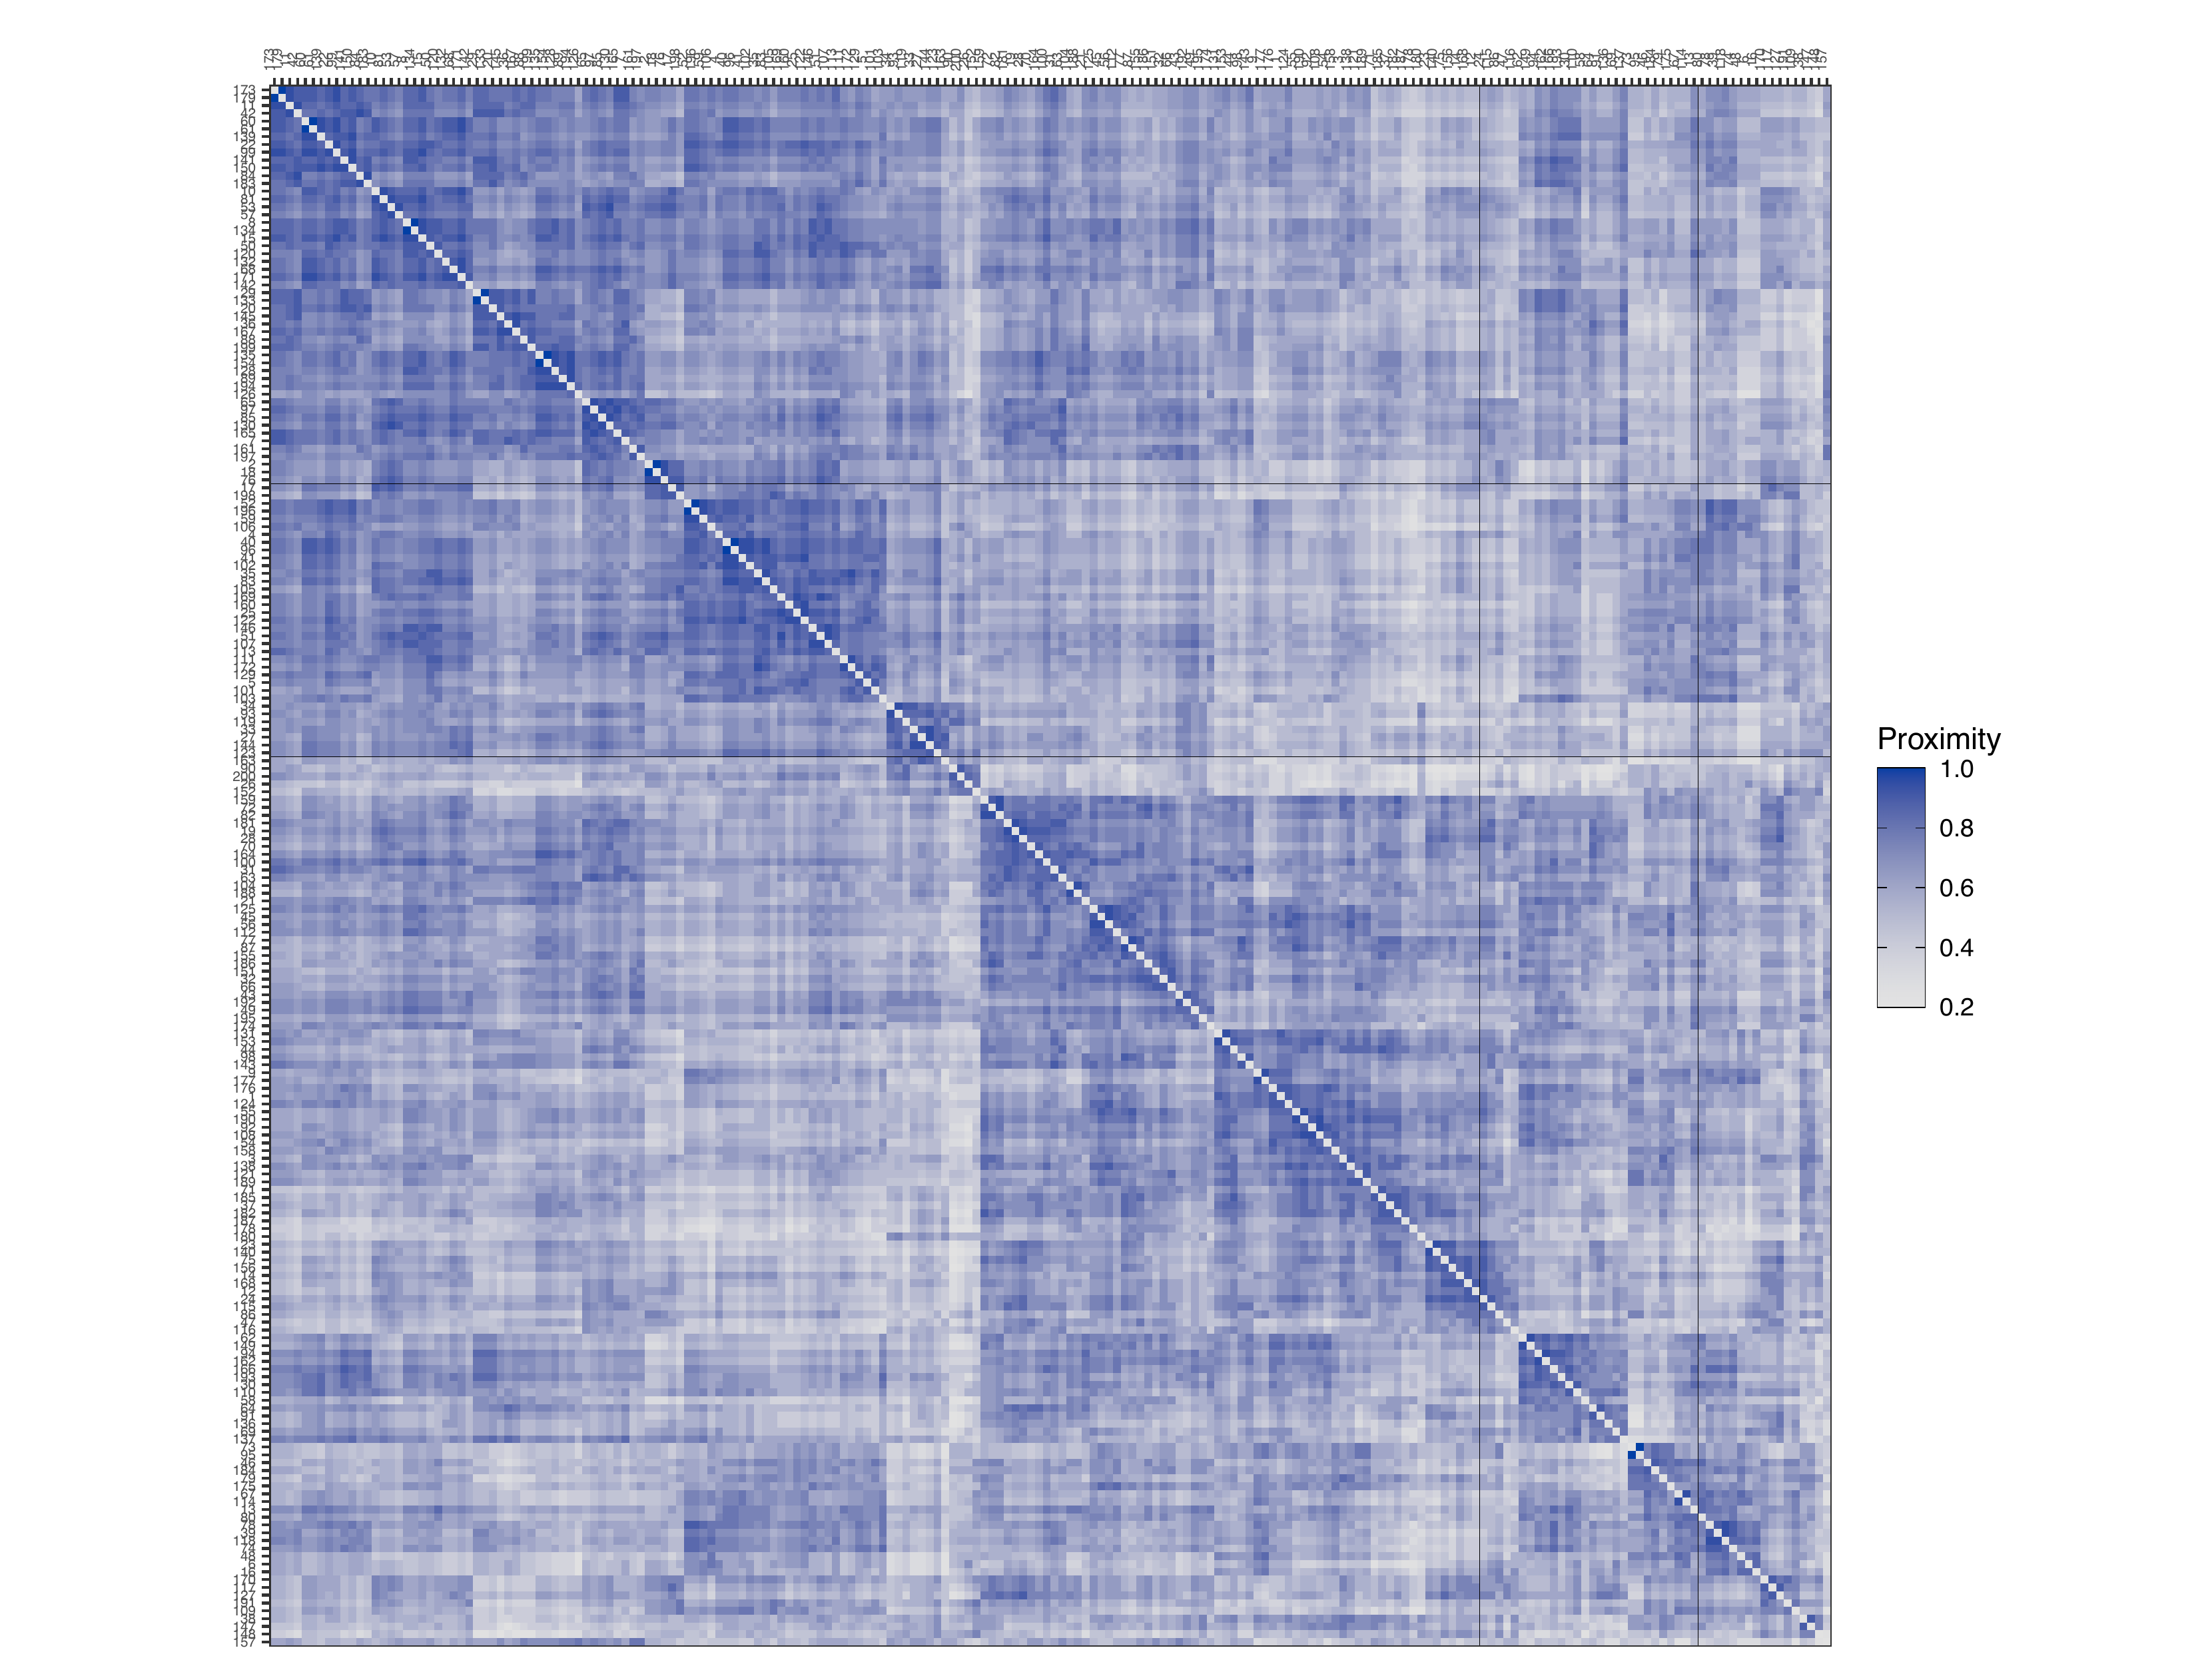
\includegraphics[width=0.8\linewidth]{https://github.com/AlanInglis/bartMan/blob/master/bartman_vignettte_new_plots_1/proximity_plot_1.png?raw=true} \end{center}

\protect\hypertarget{fig10:fig10}{}{Figure 10: }Proximity matrix
displaying only the first 50 rows and columns.

The proximity matrix can then be visualized using classical MDS
(henceforth MDS) to plot their relationship in a lower dimensional
projection.

In BART, as there is a proximity matrix for every iteration and a
posterior distribution of proximity matrices. We introduce a rotational
constraint so that we can similarly obtain a posterior distribution of
each observation in the lower dimensional space. We first choose a
target iteration (as shown above) and apply MDS. For each subsequent
iteration we rotate the MDS solution matrix to match this target as
closely as possible using Procrustes' method. We end up with a point for
each observation per iteration per MDS dimension.We then group the
observations by the mean of each group and produce a scatter plot, where
each point represents the centroid of the location of each observation
across all the MDS solutions. We extend this further by displaying the
95\% confidence ellipses around each observation's posterior location in
the reduced space. Since these are often overlapping we have created an
interactive version that highlights an observation's ellipse and
displays the observation number when hovering the mouse pointer above
the ellipse (Figure 10 shows a screenshot of this interaction in use).
However, non-interactive versions are available via the
\texttt{plotType} argument. To change the confidence ellipse size,
adjust the \texttt{level} argument.

\begin{Shaded}
\begin{Highlighting}[]
\FunctionTok{mdsBart}\NormalTok{(}\AttributeTok{treeData =}\NormalTok{ trees\_data, }\AttributeTok{data =}\NormalTok{ f\_data, }\AttributeTok{target =}\NormalTok{  bmProx,}
        \AttributeTok{plotType =} \StringTok{\textquotesingle{}interactive\textquotesingle{}}\NormalTok{, }\AttributeTok{level =} \FloatTok{0.95}\NormalTok{)}
\end{Highlighting}
\end{Shaded}

\begin{center}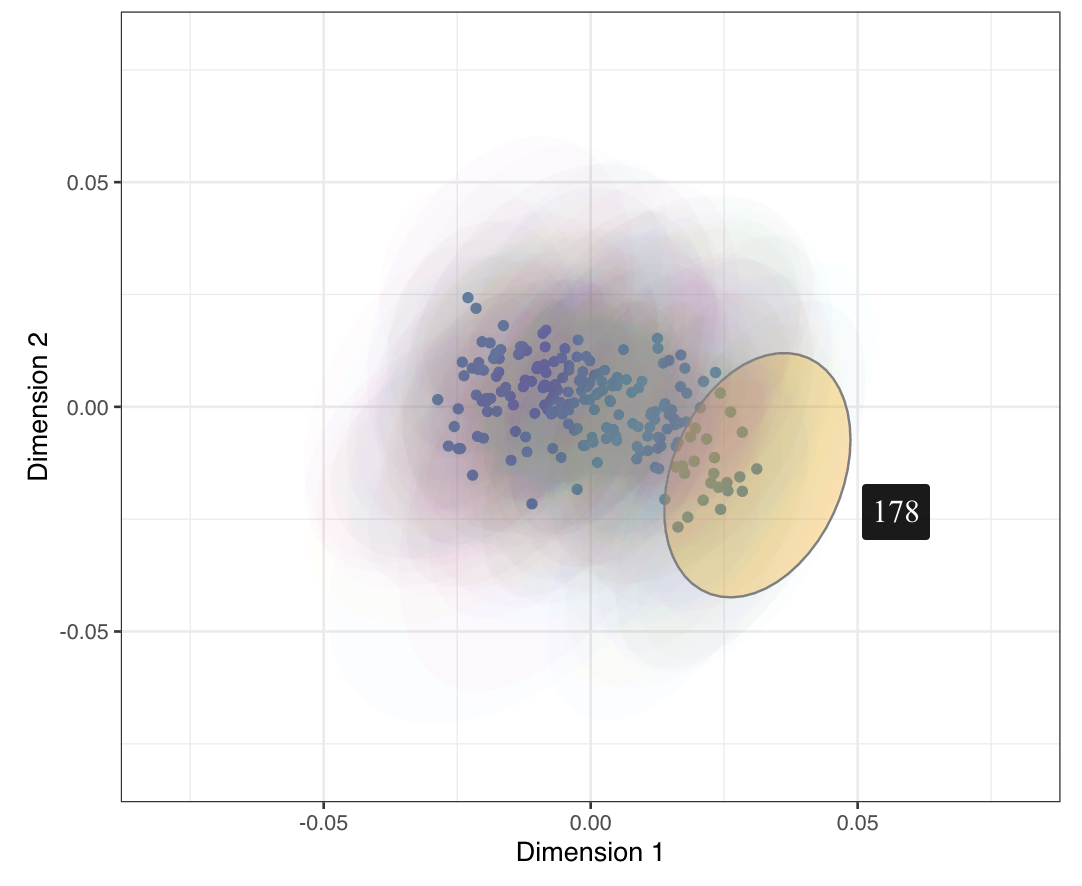
\includegraphics[width=0.8\linewidth]{https://github.com/AlanInglis/bartMan/blob/master/bartman_vignettte_new_plots_1/mds.png?raw=true} \end{center}

\protect\hypertarget{fig11:fig11}{}{Figure 11: }Interactive MDS plot.
Each 95\% confidence ellipse corresponds to each observation's posterior
location. When hovering the mouse pointer over an ellipse, the ellipse
is highlighted and the observation is displayed.

\hypertarget{enhanced-bart-model-diagnostics}{%
\subsection{Enhanced BART model
diagnostics}\label{enhanced-bart-model-diagnostics}}

In addition to the above, we also provide visualisations for general
diagnostics of a BART model. These include checking for convergence, the
stability of the trees, the efficiency of the algorithm, and the
predictive performance of the model. To begin we take a look at some
general diagnostics to assess the stability of the model fit. The
\texttt{burnIn} argument should be set to the burn-in value selected
when building the model and indicates the separation between the pre and
post burn-in period in the plot.

\begin{Shaded}
\begin{Highlighting}[]
\FunctionTok{bartDiag}\NormalTok{(}\AttributeTok{model =}\NormalTok{ dbartModel, }\AttributeTok{response =}\NormalTok{ f\_data}\SpecialCharTok{$}\NormalTok{y, }\AttributeTok{burnIn =} \DecValTok{100}\NormalTok{, }\AttributeTok{data =}\NormalTok{ fData)}
\end{Highlighting}
\end{Shaded}

\begin{center}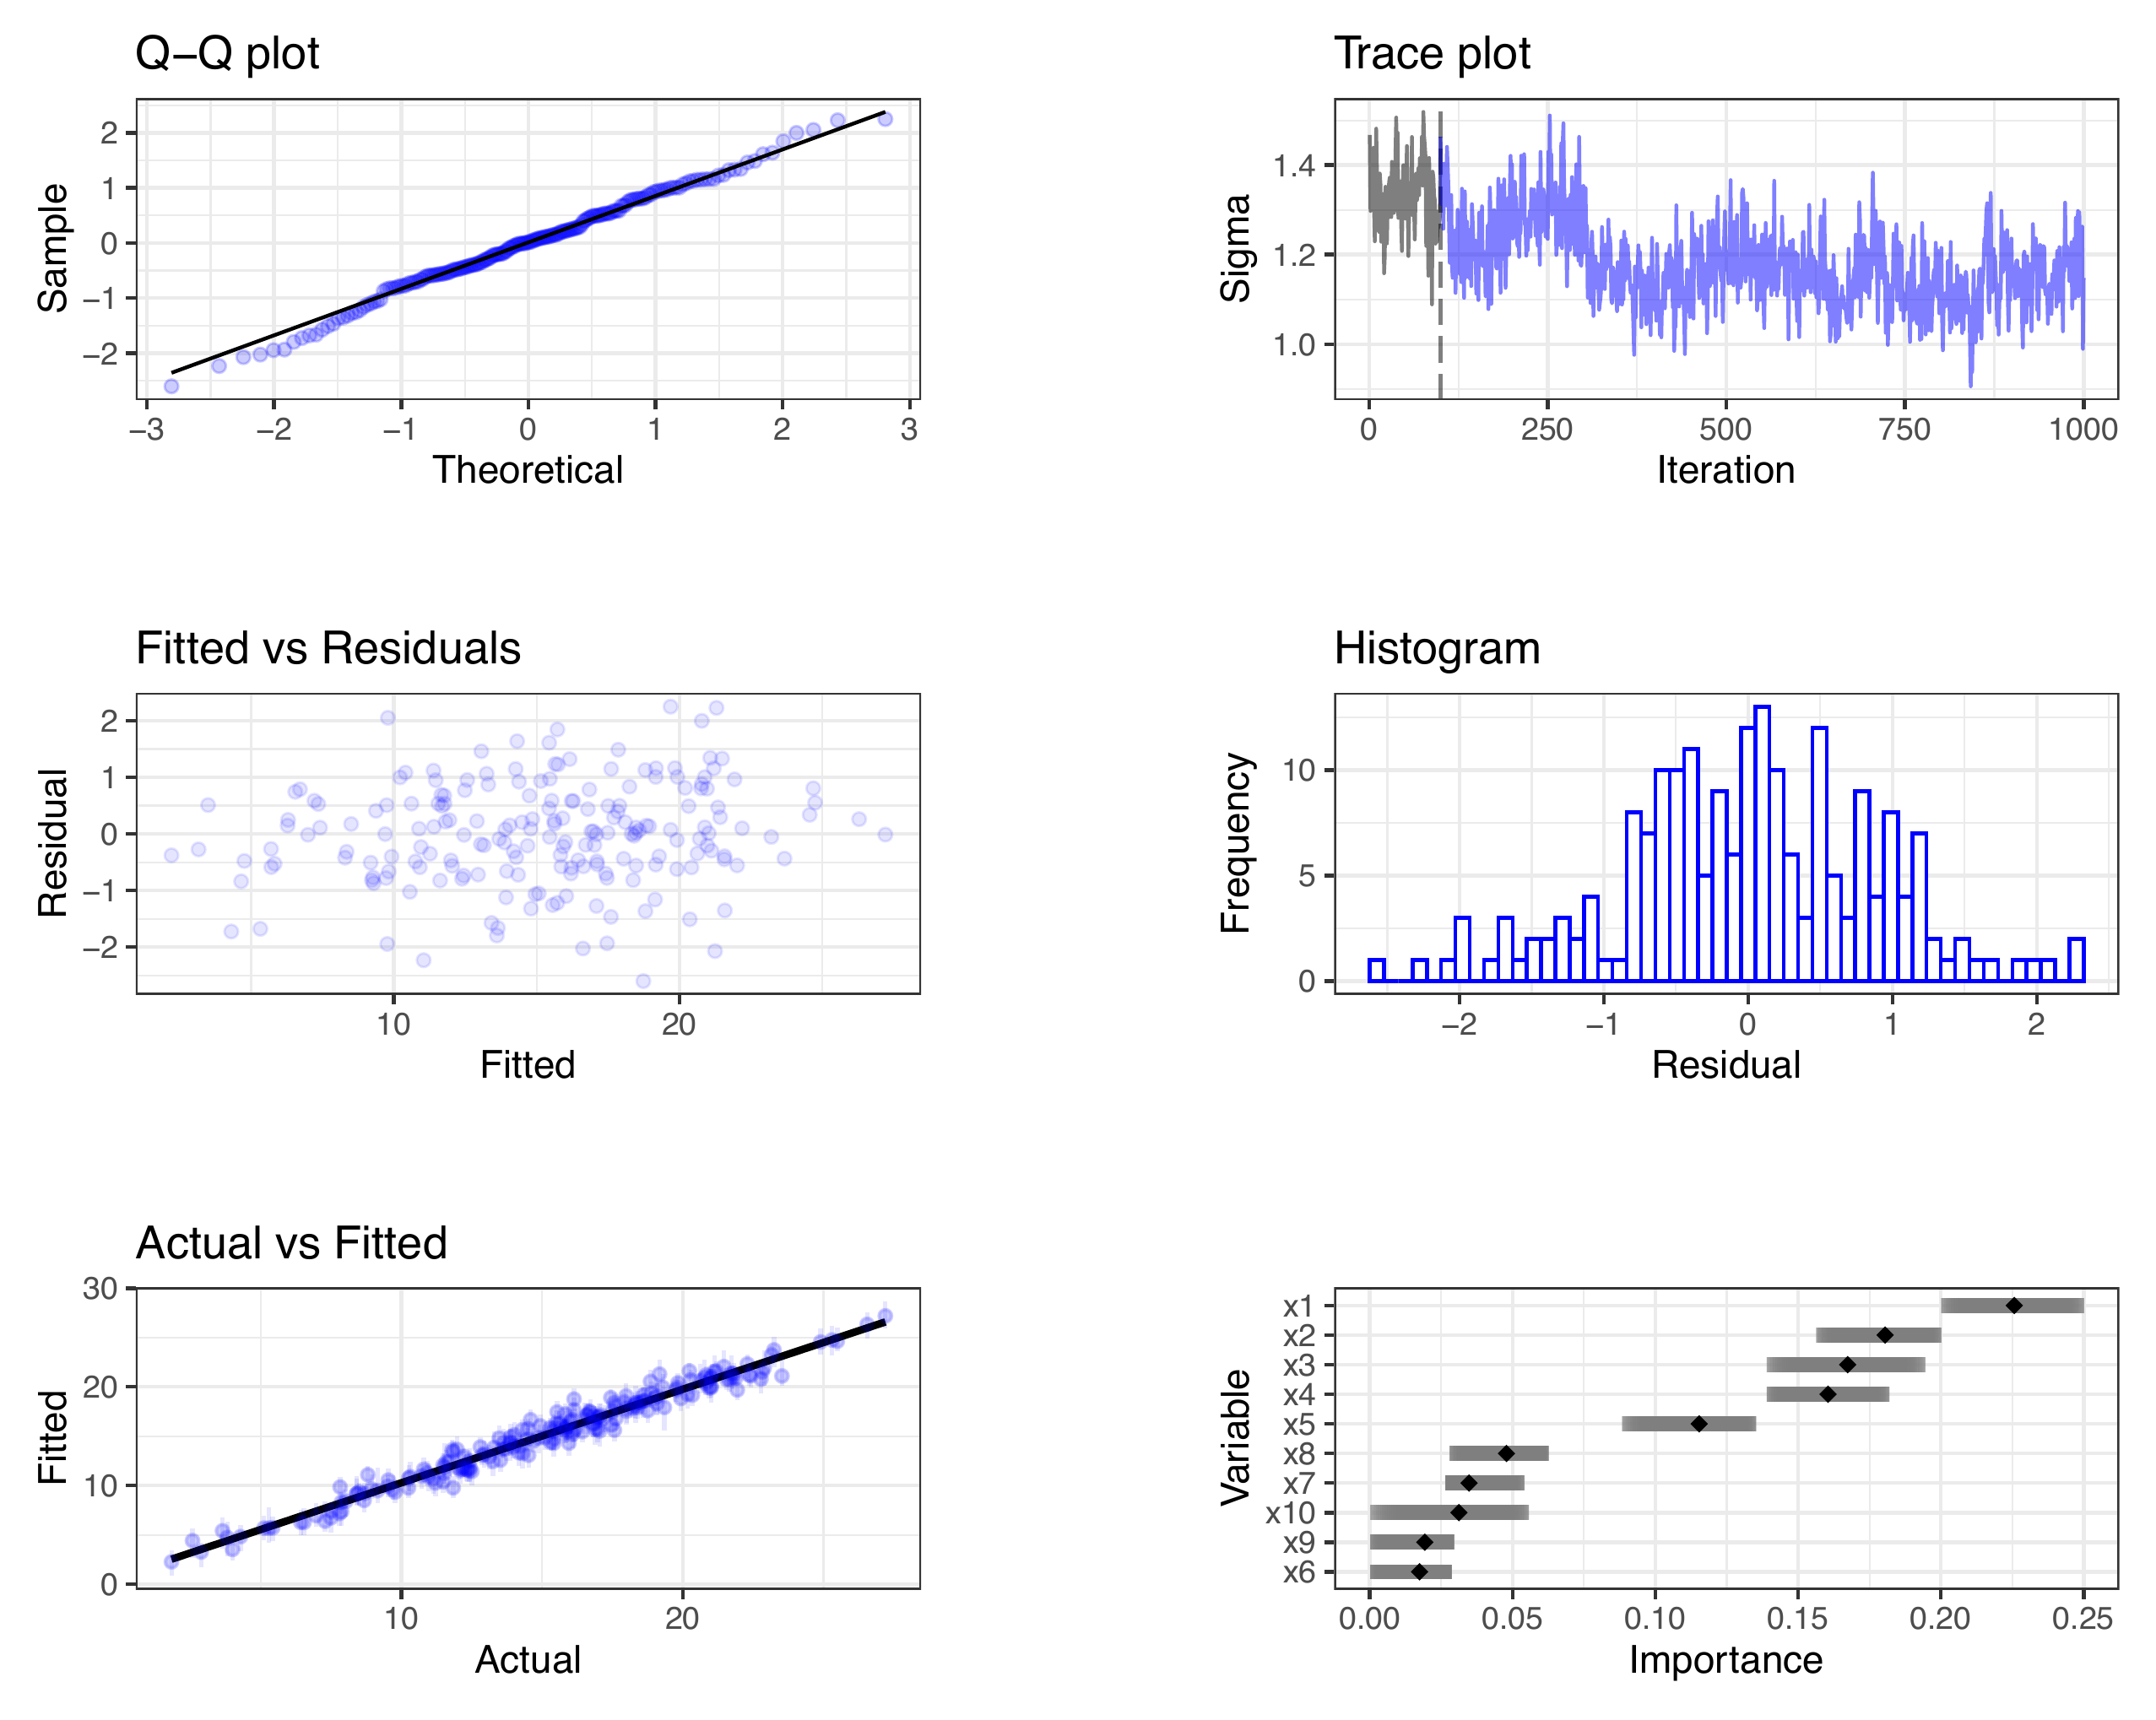
\includegraphics[width=0.8\linewidth]{https://github.com/AlanInglis/bartMan/blob/master/bartman_vignettte_new_plots_1/diagnostics_1.png?raw=true} \end{center}

\protect\hypertarget{fig12:fig12}{}{Figure 12: }General diagnostic plots
for a BART regression fit. Top left: A QQ-plot of the residuals after
fitting the model. Top right: \(\sigma\) by MCMC iteration. Middle left:
Residuals versus fitted values with 95\% credible intervals. Middle
right: A histogram of the residuals. Bottom Left: Actual values versus
fitted values with 95\% credible intervals. Bottom right: Variable
importance plot with 25 to 75\% quantile interval shown.

\hypertarget{acceptance-rate}{%
\subsubsection{Acceptance Rate}\label{acceptance-rate}}

The post burn-in percentage acceptance rate across all iterations can
also be visualized, where each point represents a single iteration. A
regression line is shown to indicate the changes in acceptance rate
across iterations and to identify the mean rate.

\begin{Shaded}
\begin{Highlighting}[]
\FunctionTok{acceptRate}\NormalTok{(}\AttributeTok{treeData =}\NormalTok{ trees\_data)}
\end{Highlighting}
\end{Shaded}

\begin{center}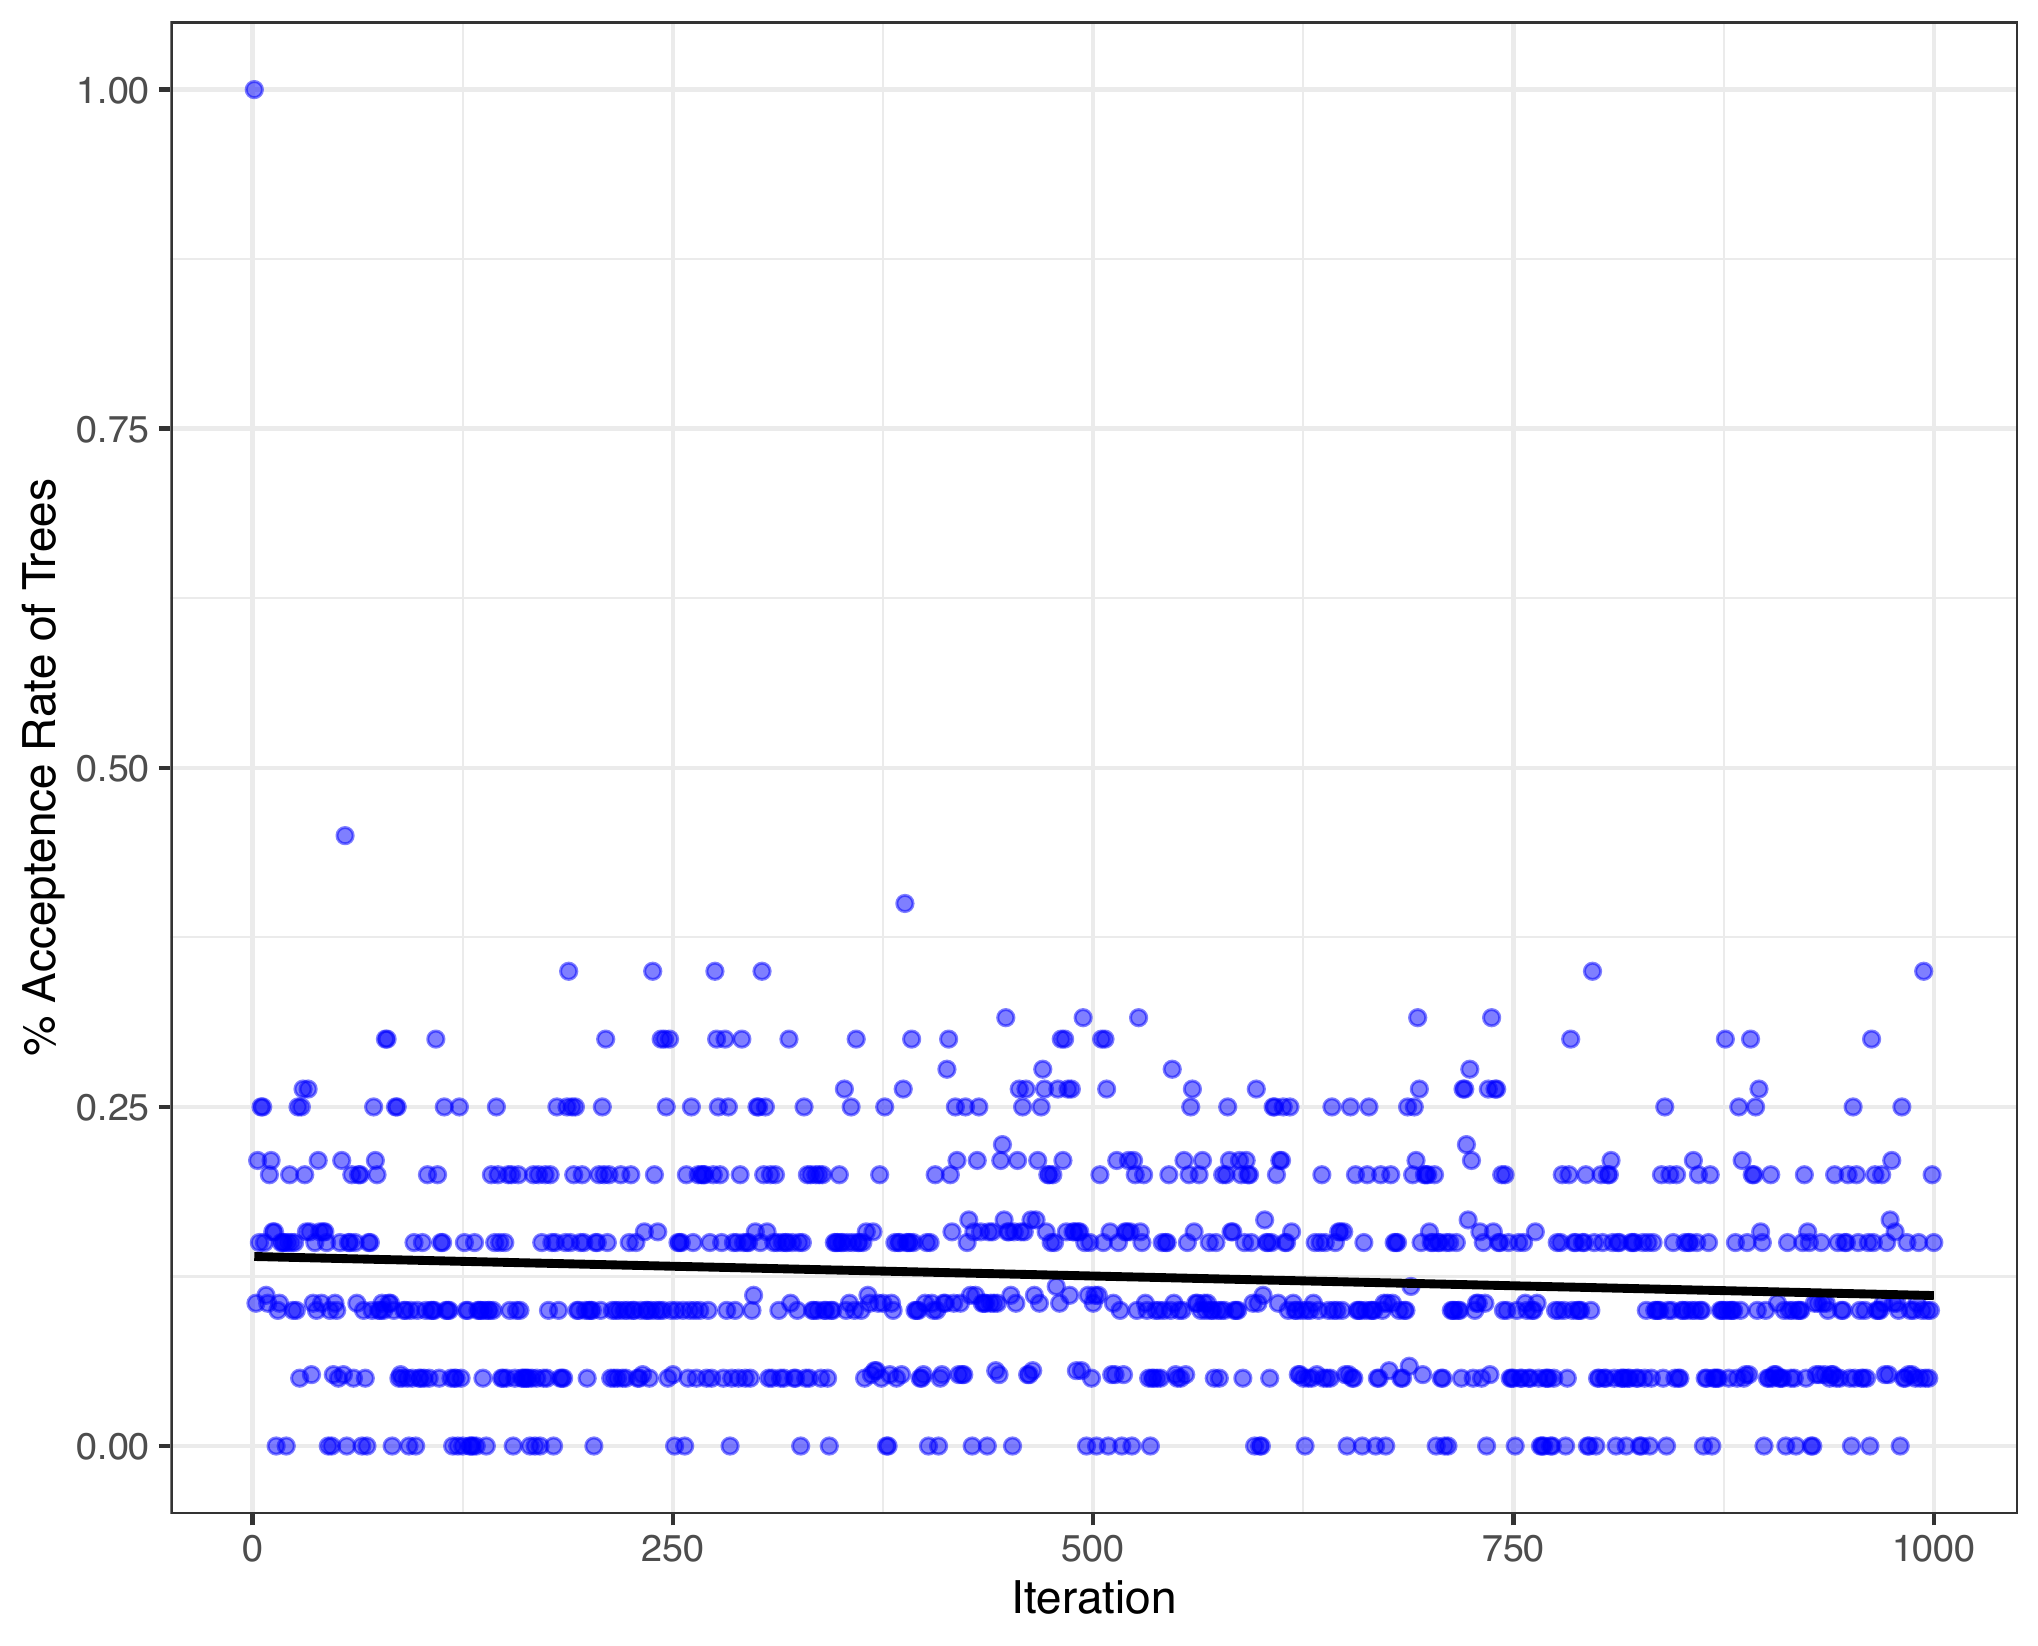
\includegraphics[width=1\linewidth]{https://github.com/AlanInglis/bartMan/blob/master/bartman_vignettte_new_plots_1/accept_rate_1.png?raw=true} \end{center}

\protect\hypertarget{fig13:fig13}{}{Figure 13: } Post burn-in acceptance
rate of trees per iteration. A black regression line is shown to
indicate the changes in acceptance rate across iterations and to
identify the mean rate.

\hypertarget{mean-tree-depth-and-mean-tree-nodes}{%
\subsubsection{Mean Tree Depth and Mean Tree
Nodes}\label{mean-tree-depth-and-mean-tree-nodes}}

As with the acceptance rate, the average tree depth and average number
of all nodes per iteration can give an insight into the fit's stability.
Figure 11 displays these two metrics. A locally estimated scatter plot
smoothing (LOESS) regression line is shown to indicate the changes in
both the average tree depth and the average number of nodes across
iterations:

\begin{Shaded}
\begin{Highlighting}[]
\FunctionTok{treeDepth}\NormalTok{(}\AttributeTok{treeData =}\NormalTok{ trees\_data)}
\FunctionTok{treeNodes}\NormalTok{(}\AttributeTok{treeData =}\NormalTok{ trees\_data)}
\end{Highlighting}
\end{Shaded}

\begin{center}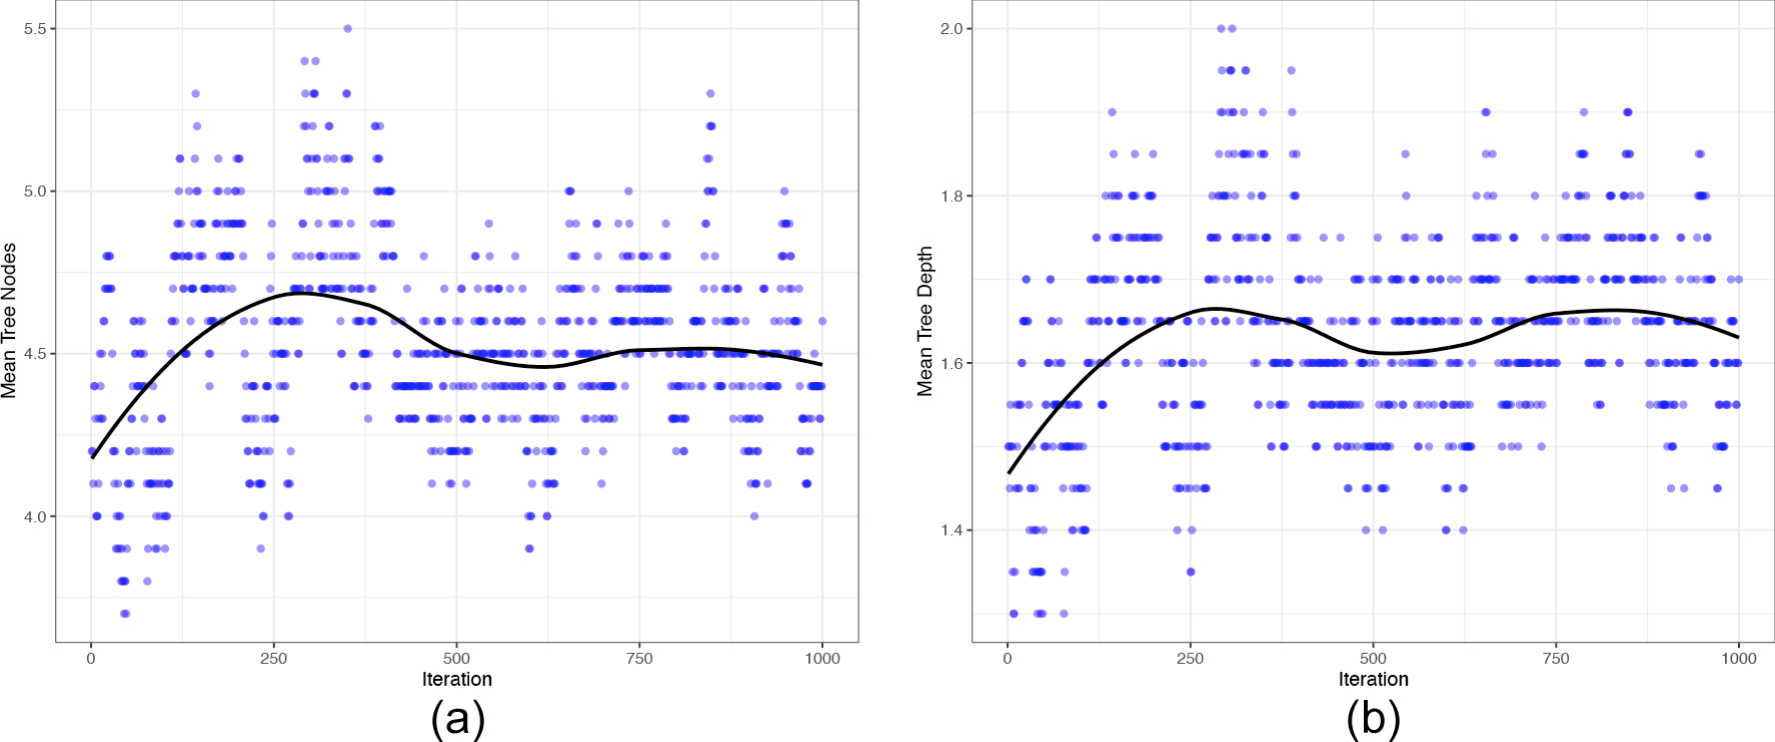
\includegraphics[width=1\linewidth]{https://github.com/AlanInglis/bartMan/blob/master/bartman_vignettte_new_plots_1/tree_depth_node_1.png?raw=true} \end{center}

\protect\hypertarget{fig14:fig14}{}{Figure 14: } In (a) we show the post
burn-in average tree depth per iteration. In (b) we show the post
burn-in average number of nodes per iteration. A black LOESS regression
curve is shown to indicate the changes in both the average tree depth
and number of nodes across iterations.

\hypertarget{split-densities}{%
\subsubsection{Split Densities}\label{split-densities}}

Figure 12 shows the densities of split values over all post burn-in
iterations for each variable for both models (in green), combined with
the densities of the predictor variables (labeled ``data'', in red):

\begin{Shaded}
\begin{Highlighting}[]
\FunctionTok{splitDensity}\NormalTok{(}\AttributeTok{treeData =}\NormalTok{ trees\_data, }\AttributeTok{data =}\NormalTok{ f\_data, }\AttributeTok{display =} \StringTok{\textquotesingle{}dataSplit\textquotesingle{}}\NormalTok{)}
\end{Highlighting}
\end{Shaded}

\begin{center}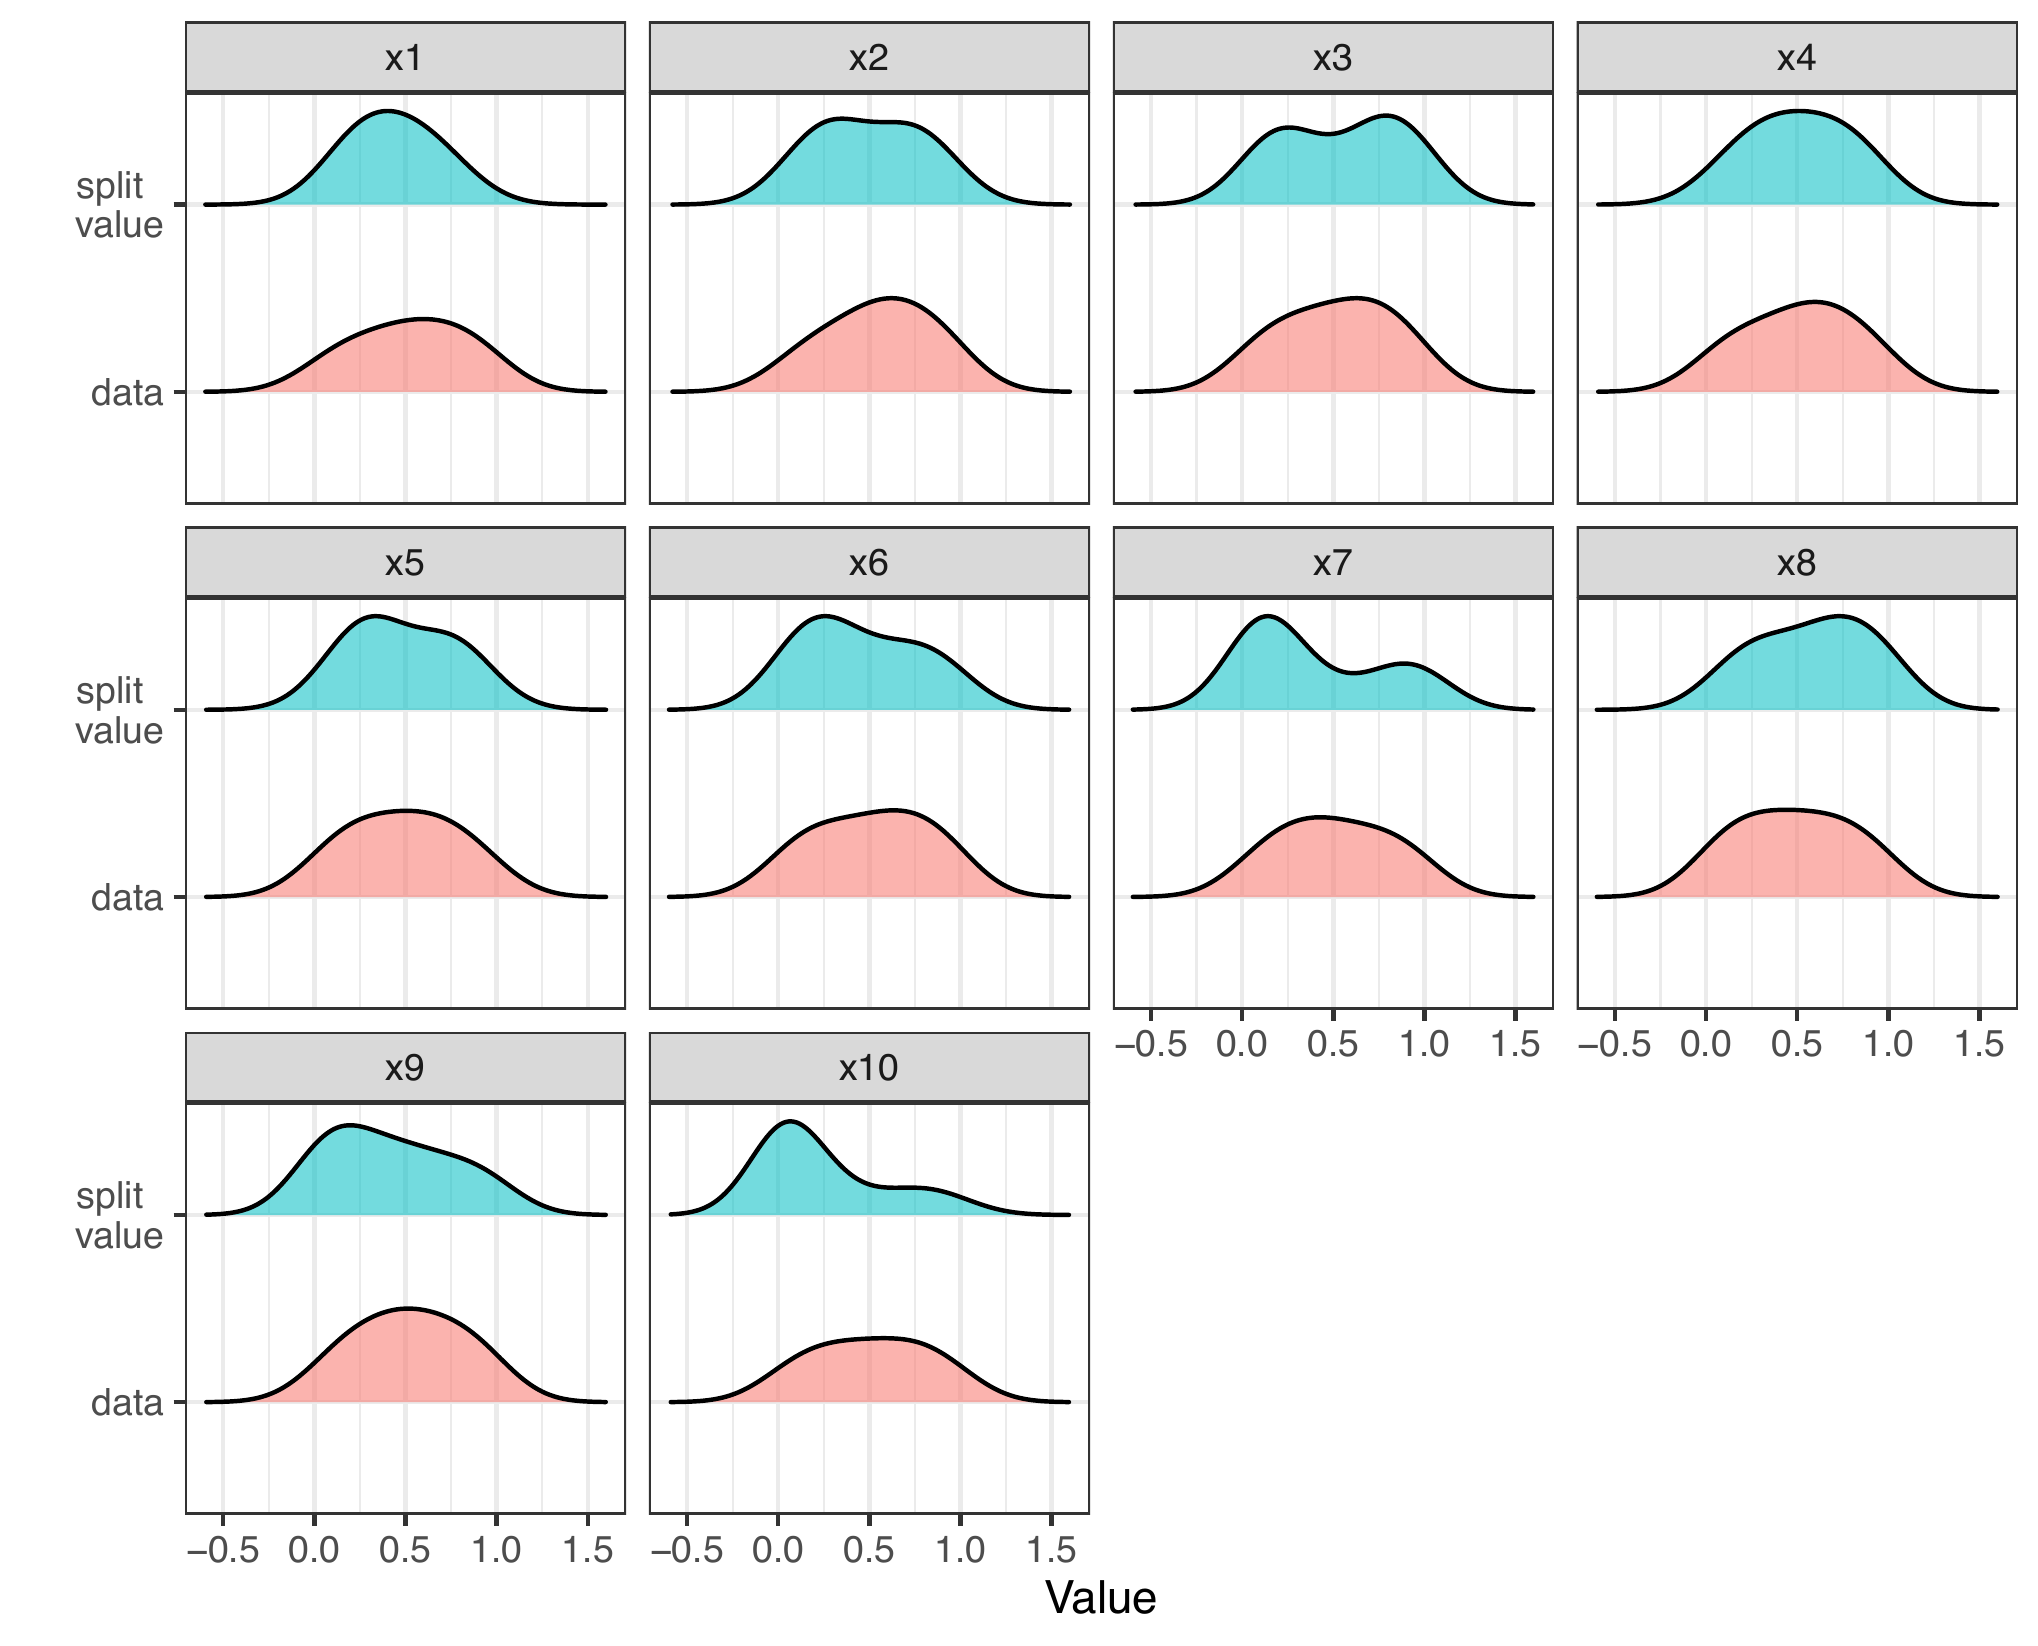
\includegraphics[width=1\linewidth]{https://github.com/AlanInglis/bartMan/blob/master/bartman_vignettte_new_plots_1/split_density_1.png?raw=true} \end{center}

\protect\hypertarget{fig15:fig15}{}{Figure 15: } Split values densities
(in green) over all iterations for each variable overlayed on the
densities of the predictors (in red).

\begin{Shaded}
\begin{Highlighting}[]
\FunctionTok{splitDensity}\NormalTok{(}\AttributeTok{treeData =}\NormalTok{ trees\_data, }\AttributeTok{data =}\NormalTok{ f\_data, }\AttributeTok{display =} \StringTok{\textquotesingle{}ridges\textquotesingle{}}\NormalTok{)}
\end{Highlighting}
\end{Shaded}

\begin{center}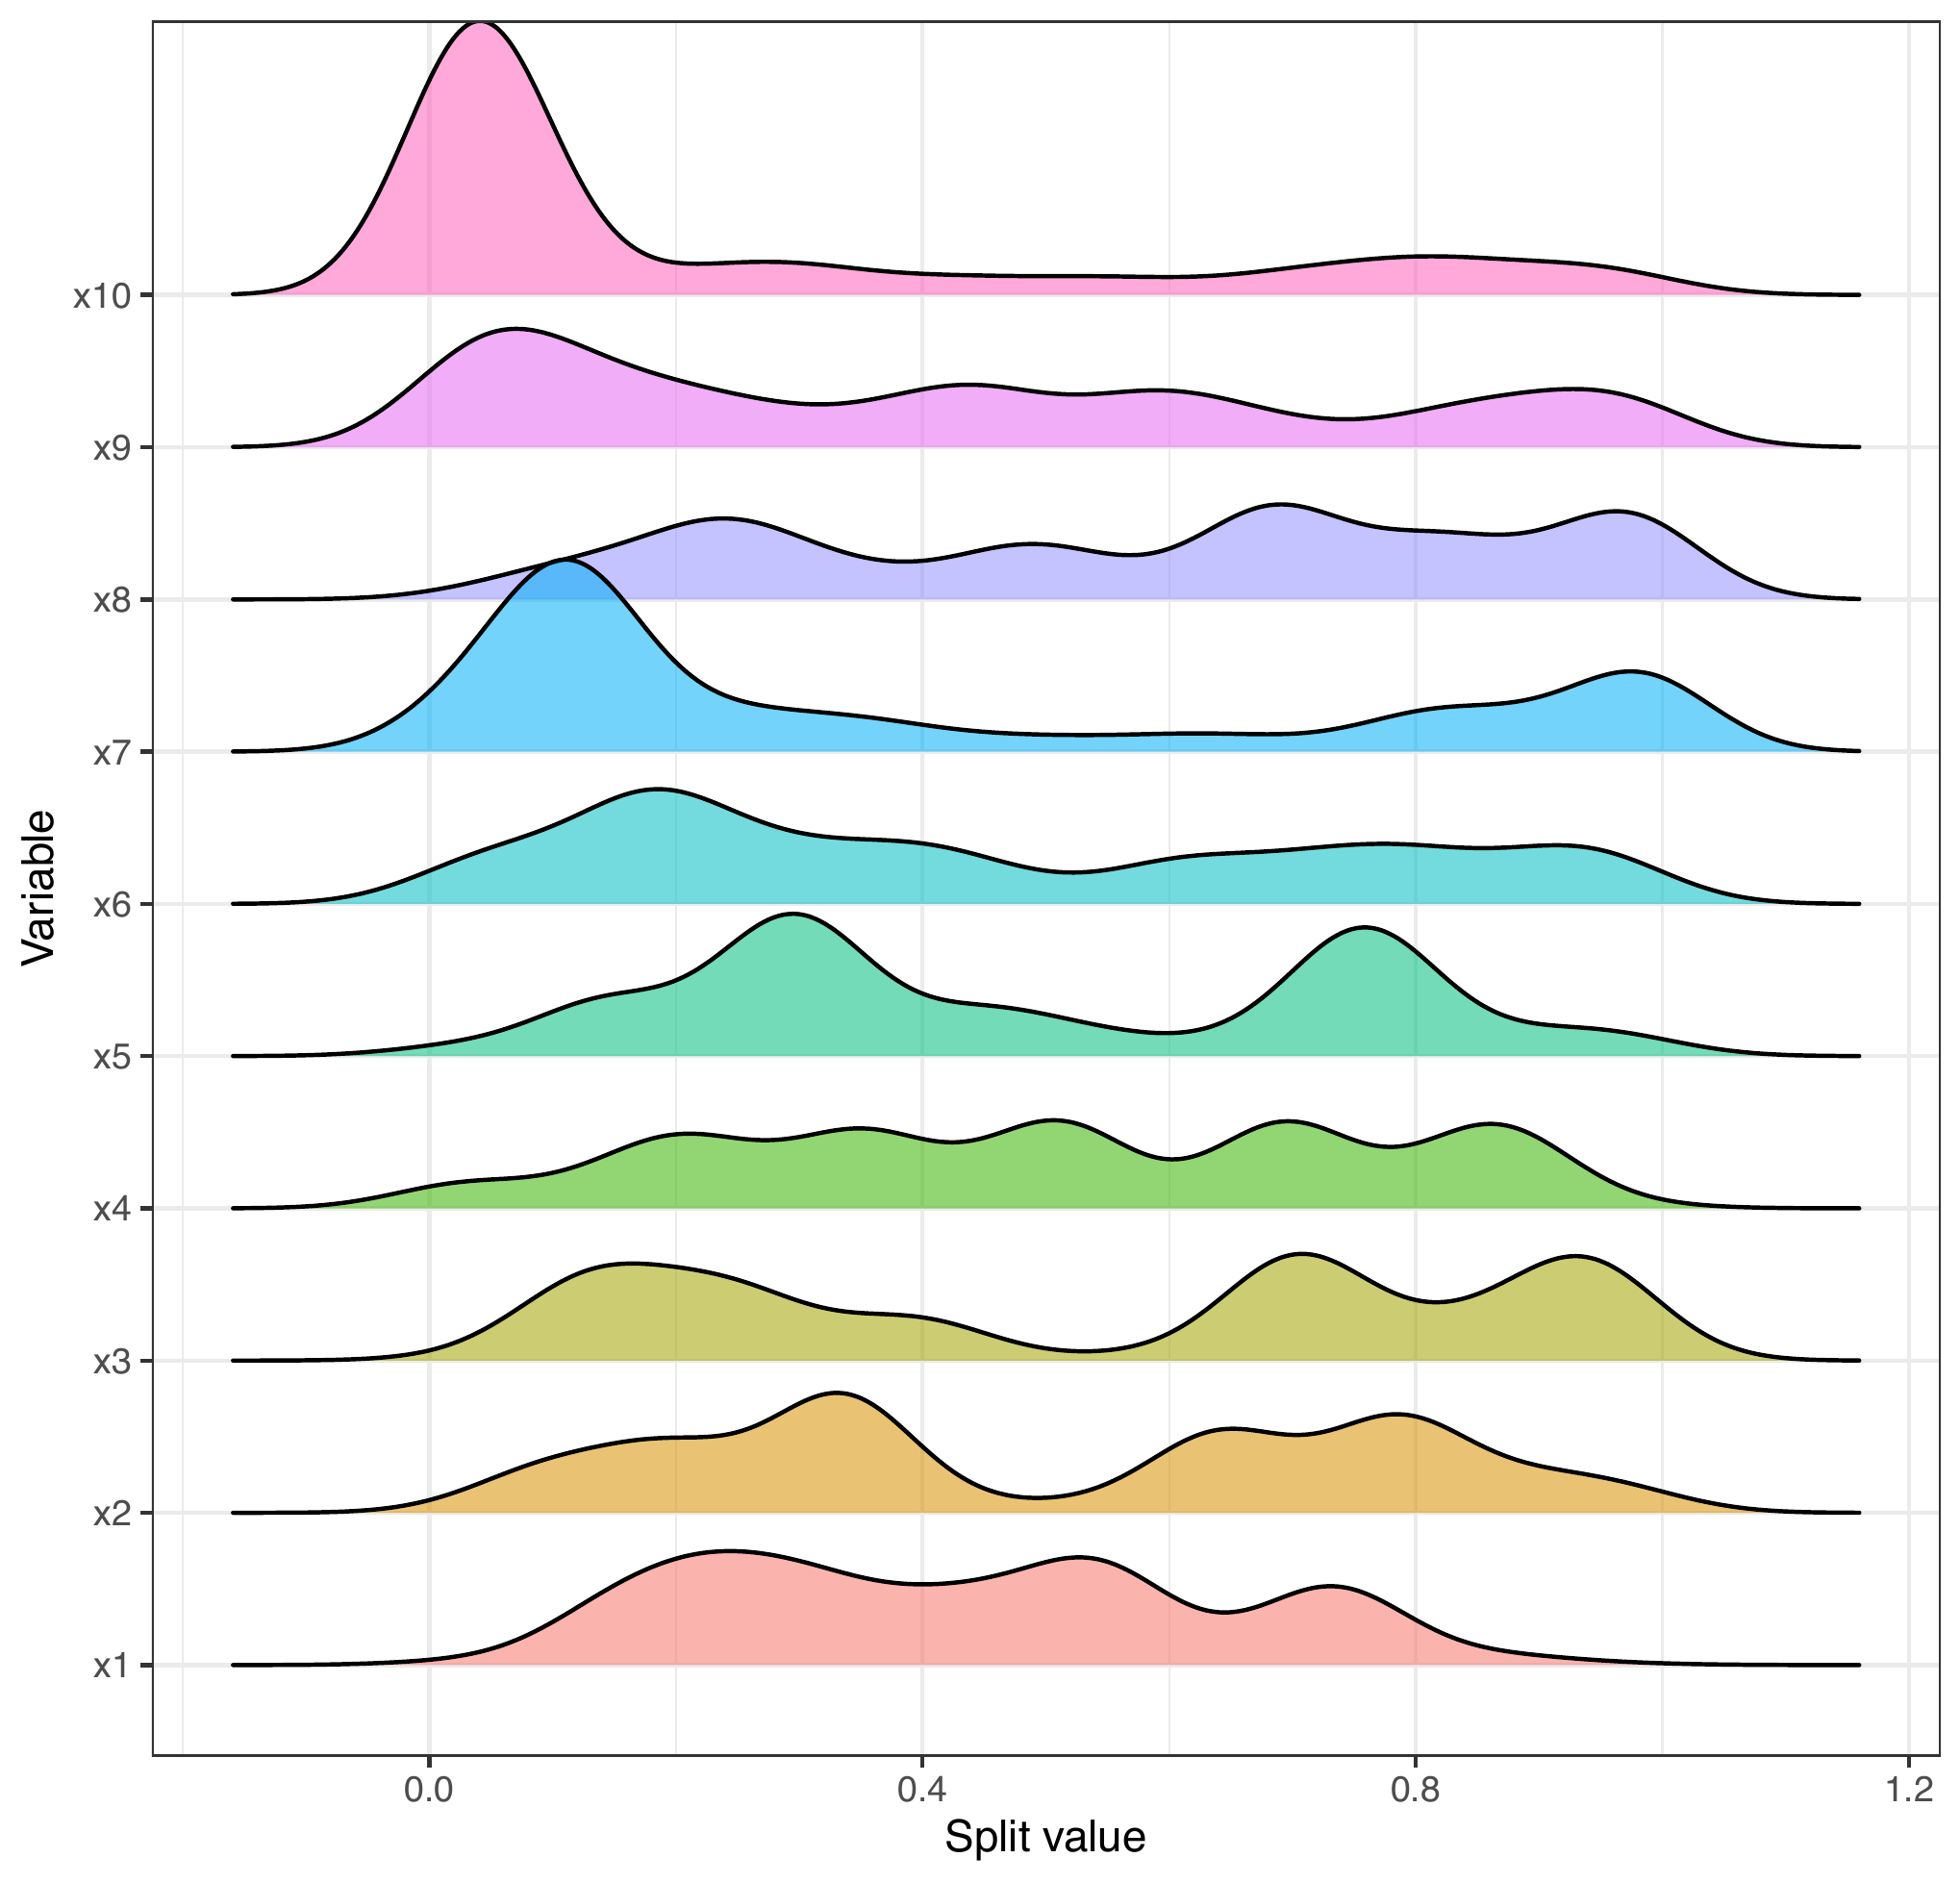
\includegraphics[width=1\linewidth]{https://github.com/AlanInglis/bartMan/blob/master/bartman_vignettte_new_plots_1/ridges_1.png?raw=true} \end{center}

\protect\hypertarget{fig16:fig16}{}{Figure 16: } Split values densities
XXXXXXXXXXXXXXXXX.

\hypertarget{additional-importance-and-interaction-plots.}{%
\subsection{Additional Importance and Interaction
plots.}\label{additional-importance-and-interaction-plots.}}

The assess the inclusion proportions for use with variable importance or
variable interactions. We also provide some useful functions for
extracting these values and for visualizing them. For example, to
retrieve a list containing both the variable importance and variable
interactions (and associated error metrics) we can use the
\texttt{viviBart} function. To select either just the importance or just
the interactions, we set the \texttt{out} argument to `vimp' or vint'
respectively. The \texttt{combineFact} argument is discussed in greater
detail below.

\begin{Shaded}
\begin{Highlighting}[]
\CommentTok{\# show both vimp and vint}
\FunctionTok{viviBart}\NormalTok{(}\AttributeTok{treeData =}\NormalTok{ trees\_data, }\AttributeTok{out =} \StringTok{\textquotesingle{}vivi\textquotesingle{}}\NormalTok{)}
\CommentTok{\#\textgreater{} $Vimp}
\CommentTok{\#\textgreater{}     variable count   propMean         SD        CV         SE       lowerCI}
\CommentTok{\#\textgreater{} x1        x1    18 0.26162698 0.08237503 0.3148568 0.02604927  2.105704e{-}01}
\CommentTok{\#\textgreater{} x2        x2    11 0.16087302 0.06493273 0.4036272 0.02053353  1.206273e{-}01}
\CommentTok{\#\textgreater{} x3        x3     0 0.00000000 0.00000000 0.0000000 0.00000000  0.000000e+00}
\CommentTok{\#\textgreater{} x4        x4    26 0.35928571 0.09868243 0.2746628 0.03120612  2.981217e{-}01}
\CommentTok{\#\textgreater{} x5        x5     7 0.09325397 0.06520507 0.6992203 0.02061965  5.283945e{-}02}
\CommentTok{\#\textgreater{} x6        x6     1 0.02000000 0.06324555 3.1622777 0.02000000 {-}1.920000e{-}02}
\CommentTok{\#\textgreater{} x7        x7     2 0.02678571 0.05662589 2.1140331 0.01790668 {-}8.311373e{-}03}
\CommentTok{\#\textgreater{} x8        x8     3 0.03611111 0.05826716 1.6135521 0.01842569 {-}3.247717e{-}06}
\CommentTok{\#\textgreater{} x9        x9     0 0.00000000 0.00000000 0.0000000 0.00000000  0.000000e+00}
\CommentTok{\#\textgreater{} x10      x10     3 0.04206349 0.06899134 1.6401715 0.02181698 {-}6.977842e{-}04}
\CommentTok{\#\textgreater{}        upperCI     lowerQ    median     upperQ}
\CommentTok{\#\textgreater{} x1  0.31268356 0.22916667 0.2857143 0.28571429}
\CommentTok{\#\textgreater{} x2  0.20111874 0.12946429 0.1428571 0.14285714}
\CommentTok{\#\textgreater{} x3  0.00000000 0.00000000 0.0000000 0.00000000}
\CommentTok{\#\textgreater{} x4  0.42044972 0.34375000 0.4017857 0.42857143}
\CommentTok{\#\textgreater{} x5  0.13366849 0.02777778 0.1250000 0.14285714}
\CommentTok{\#\textgreater{} x6  0.05920000 0.00000000 0.0000000 0.00000000}
\CommentTok{\#\textgreater{} x7  0.06188280 0.00000000 0.0000000 0.00000000}
\CommentTok{\#\textgreater{} x8  0.07222547 0.00000000 0.0000000 0.08333333}
\CommentTok{\#\textgreater{} x9  0.00000000 0.00000000 0.0000000 0.00000000}
\CommentTok{\#\textgreater{} x10 0.08482477 0.00000000 0.0000000 0.08333333}
\CommentTok{\#\textgreater{} }
\CommentTok{\#\textgreater{} $Vint}
\CommentTok{\#\textgreater{} \# A tibble: 55 x 10}
\CommentTok{\#\textgreater{}    var    count propMean     SD    CV     SE lowerQ median upperQ adjusted}
\CommentTok{\#\textgreater{}    \textless{}chr\textgreater{}  \textless{}dbl\textgreater{}    \textless{}dbl\textgreater{}  \textless{}dbl\textgreater{} \textless{}dbl\textgreater{}  \textless{}dbl\textgreater{}  \textless{}dbl\textgreater{}  \textless{}dbl\textgreater{}  \textless{}dbl\textgreater{}    \textless{}dbl\textgreater{}}
\CommentTok{\#\textgreater{}  1 x1:x1    0     0      0      0     0      0       0       0      0     }
\CommentTok{\#\textgreater{}  2 x1:x2    0.7   0.179  0.157  0.877 0.0497 0.0312  0.208   0.25   0.668 }
\CommentTok{\#\textgreater{}  3 x1:x3    0     0      0      0     0      0       0       0      0     }
\CommentTok{\#\textgreater{}  4 x1:x4    0     0      0      0     0      0       0       0      0     }
\CommentTok{\#\textgreater{}  5 x1:x5    0     0      0      0     0      0       0       0      0     }
\CommentTok{\#\textgreater{}  6 x1:x6    0     0      0      0     0      0       0       0      0     }
\CommentTok{\#\textgreater{}  7 x1:x7    0     0      0      0     0      0       0       0      0     }
\CommentTok{\#\textgreater{}  8 x1:x8    0     0      0      0     0      0       0       0      0     }
\CommentTok{\#\textgreater{}  9 x1:x9    0     0      0      0     0      0       0       0      0     }
\CommentTok{\#\textgreater{} 10 x1:x10   0.1   0.0125 0.0395 3.16  0.0125 0       0       0      0.0143}
\CommentTok{\#\textgreater{} \# i 45 more rows}
\end{Highlighting}
\end{Shaded}

To visualize the inclusion proportion variable importance (with their
25\% to 75\% quantile interval included) we use the \texttt{vimpPlot}
function.

\begin{Shaded}
\begin{Highlighting}[]
\CommentTok{\# plot inclusion proportions of each variable:}
\FunctionTok{vimpPlot}\NormalTok{(}\AttributeTok{treeData =}\NormalTok{ trees\_data, }\AttributeTok{plotType =} \StringTok{\textquotesingle{}point\textquotesingle{}}\NormalTok{)}
\FunctionTok{vimpPlot}\NormalTok{(}\AttributeTok{treeData =}\NormalTok{ trees\_data, }\AttributeTok{plotType =} \StringTok{\textquotesingle{}barplot\textquotesingle{}}\NormalTok{)}
\end{Highlighting}
\end{Shaded}

\begin{center}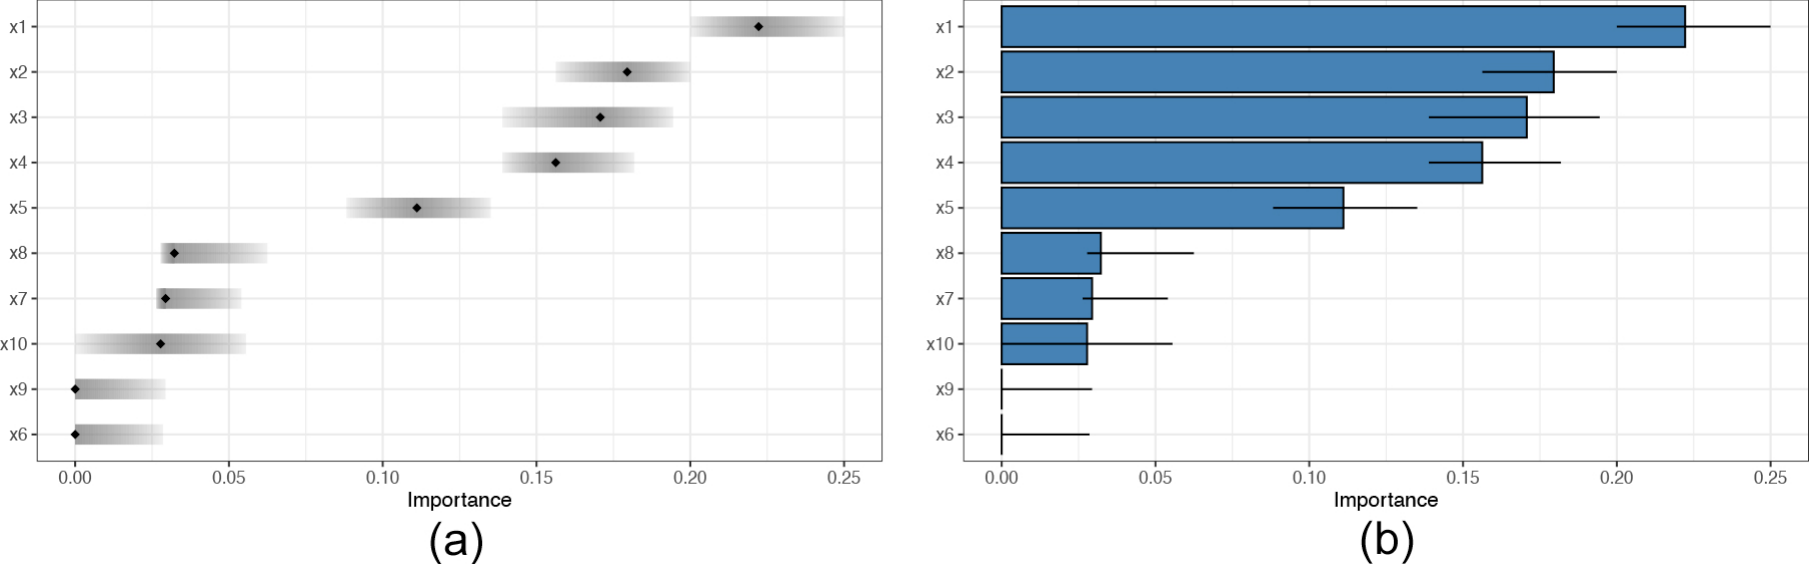
\includegraphics[width=1\linewidth,height=1\textheight]{https://github.com/AlanInglis/bartMan/blob/master/bartman_vignettte_new_plots_1/vimp_point_bar_1.png?raw=true} \end{center}

\protect\hypertarget{fig17:fig17}{}{Figure 17: } Inclusion proportions
for each variable shown with the 25\% to 75\% quantile interval
extending from the points.

An alternative method to display the inclusion proportions is by using a
\emph{Letter-value plot}\footnote{Hofmann, H., Wickham, H., \& Kafadar,
  K. (2017). value plots: Box plots for large data. Journal of
  Computational and Graphical Statistics, 26(3), 469-477.}. This type of
plot is useful for visualizing the distribution of a continuous variable
(here variable inclusion proportions), with the inner-most box showing
the lower and upper fourths, as with a conventional box plot, the median
value being shown as a black line and outliers as blue triangles. Each
extending section is drawn at incremental steps of upper and lower
eights, sixteenths and so on until a stopping rule has been reached. The
color of each box corresponds to the density of the data with darker
shades indicating higher data density.

\begin{Shaded}
\begin{Highlighting}[]
\FunctionTok{vimpPlot}\NormalTok{(}\AttributeTok{treeData =}\NormalTok{ trees\_data, }\AttributeTok{plotType =} \StringTok{\textquotesingle{}lvp\textquotesingle{}}\NormalTok{) }\SpecialCharTok{+} \FunctionTok{coord\_flip}\NormalTok{()}
\end{Highlighting}
\end{Shaded}

\begin{center}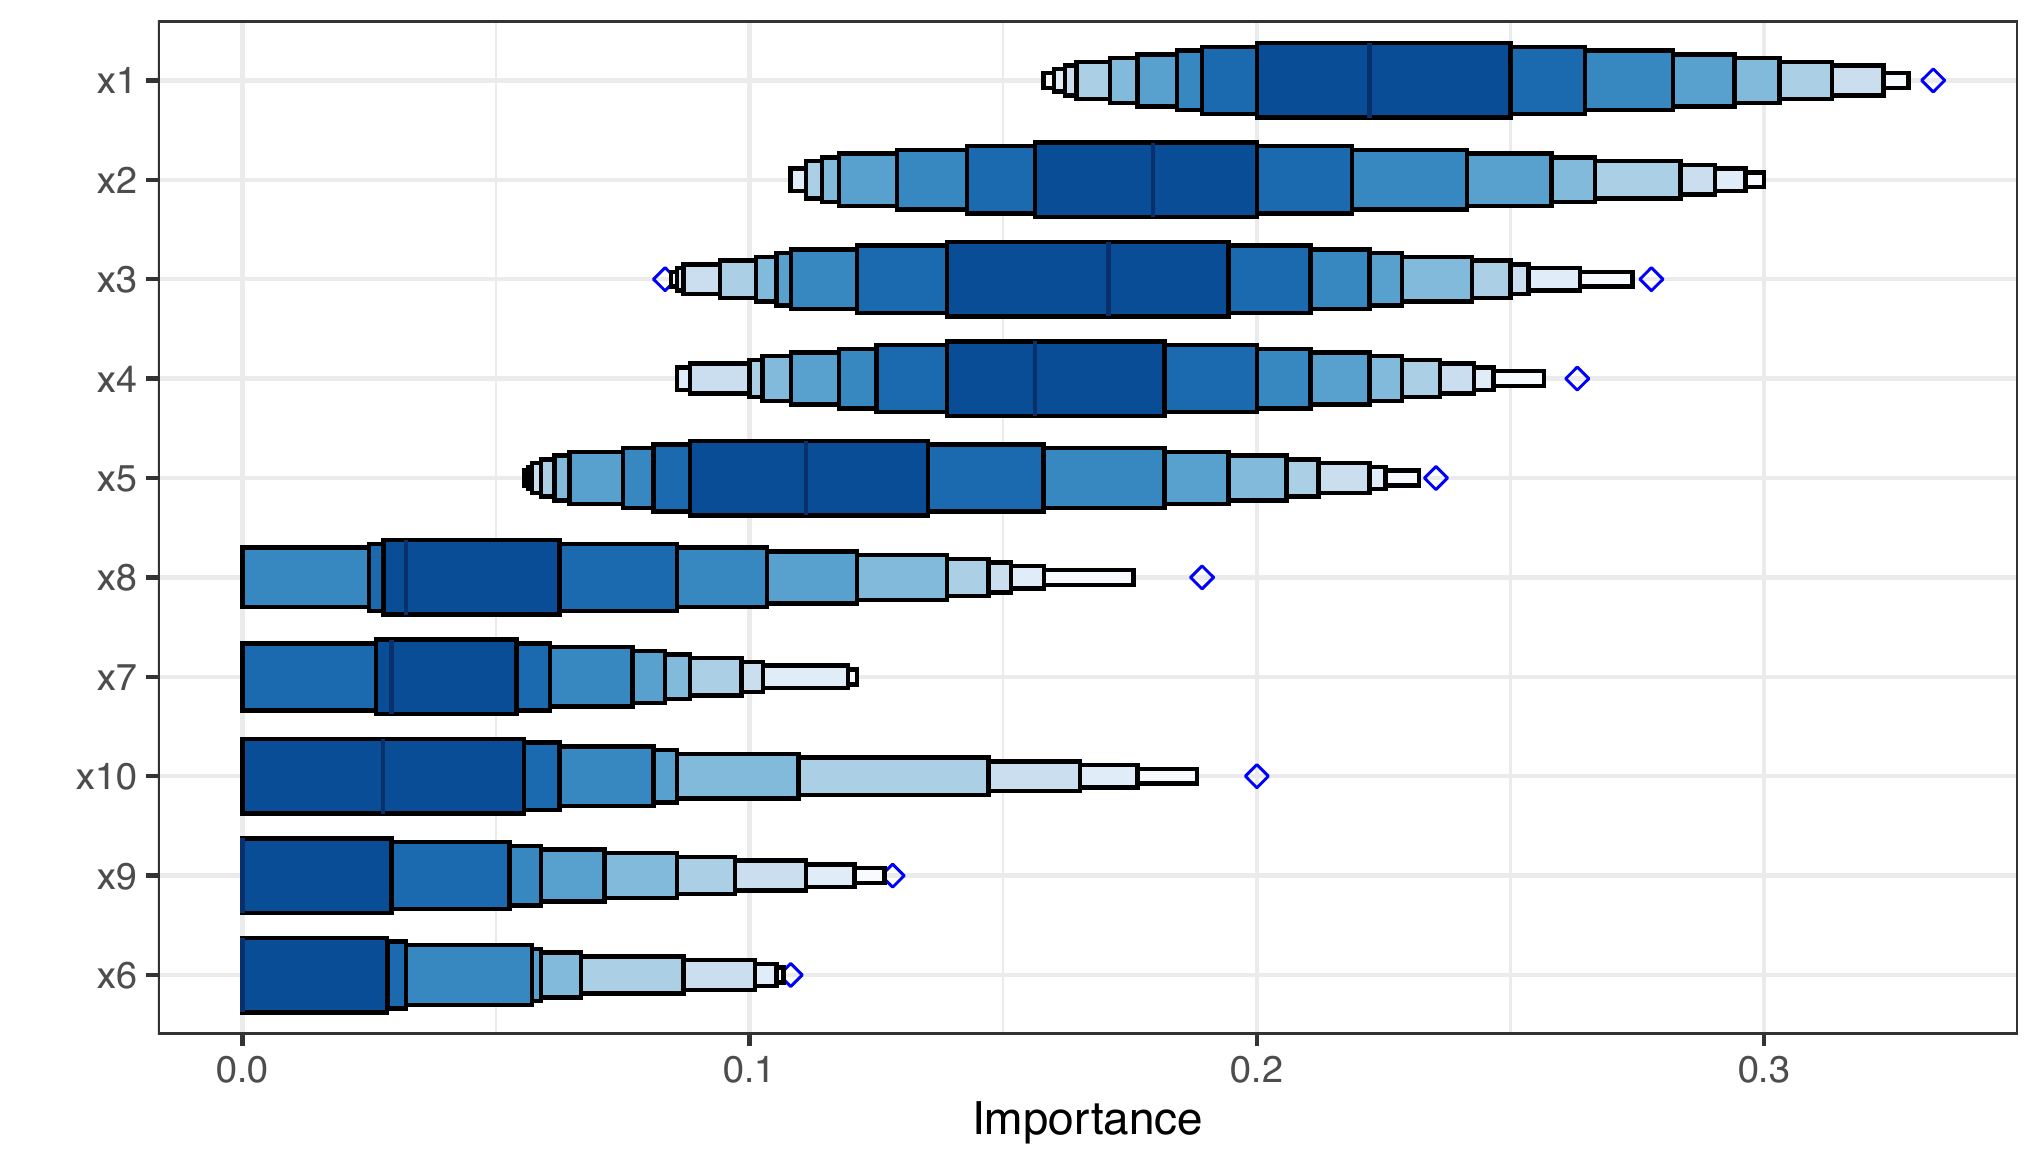
\includegraphics[width=1\linewidth]{https://github.com/AlanInglis/bartMan/blob/master/bartman_vignettte_new_plots_1/vimp_lvp_1.png?raw=true} \end{center}

\protect\hypertarget{fig18:fig18}{}{Figure 18: } Letter-value plot of
the inclusion proportions for each variable.

Similarly, we provide a function for viewing the inclusion proportions
for interactions (this time displayed as a barplot, again with 25\% to
75\% quantile interval included):

\begin{Shaded}
\begin{Highlighting}[]
\CommentTok{\# plot inclusion proportions of each variable pair:}
\FunctionTok{vintPlot}\NormalTok{(}\AttributeTok{treeData =}\NormalTok{ trees\_data, }\AttributeTok{top =} \DecValTok{5}\NormalTok{)}
\end{Highlighting}
\end{Shaded}

\begin{center}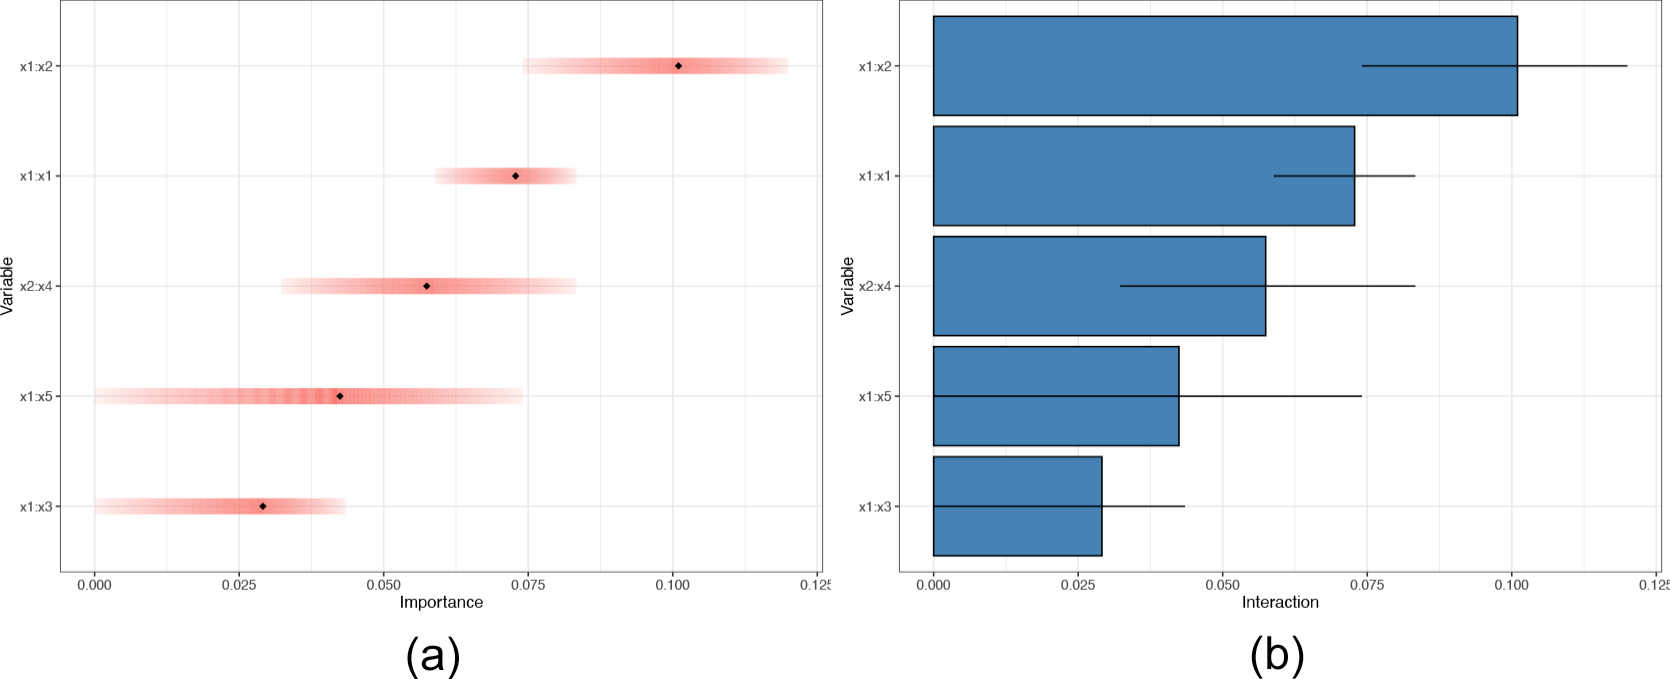
\includegraphics[width=1\linewidth]{https://github.com/AlanInglis/bartMan/blob/master/bartman_vignettte_new_plots_1/vint_point_bar_1.png?raw=true} \end{center}

\protect\hypertarget{fig19:fig19}{}{Figure 19: } Inclusion proportions
for each variable pair shown with the 25\% to 75\% quantile interval
extending from the bars

\hypertarget{null-model-inclusion-proportions}{%
\subsection{Null model inclusion
proportions}\label{null-model-inclusion-proportions}}

In our package we also implement one of the variable selection
procedures developed in Bleich et al.~(2014)\footnote{Bleich, J.,
  Kapelner, A., George, E. I., \& Jensen, S. T. (2014). Variable
  selection for BART: an application to gene regulation. The Annals of
  Applied Statistics, 8(3), 1750-1781.}, specifically, the so-called
\emph{local threshold procedure}. In this method, the proportion of
splitting rules is calculated, then the response variable is randomly
permuted, which has the effect of breaking the relationship between the
response and the covariates. The model is then re-built as a \emph{null}
model using the permuted response. From this, the null proportion, is
calculated and a new measure of importance is obtained.

When using this method, there are three key arguments: \texttt{numRep},
\texttt{numTreesRep}, and \texttt{alpha}. \texttt{numRep} determines the
number of replicates to perform for the BART null model's variable
inclusion proportions. Whereas, \texttt{numTreesRep} determines the
number of trees to be used in the replicates. \texttt{alpha} sets the
cut-off level for the thresholds. That is, a predictor is deemed
important if its variable inclusion proportion exceeds the 1 −
\(\alpha\) quantile of its own null distribution. If setting
\texttt{shift\ =\ TRUE}, the inclusion proportions are shifted by the
difference in distance between the quantile and the value of the
inclusion proportion point.

\begin{Shaded}
\begin{Highlighting}[]
\FunctionTok{localProcedure}\NormalTok{(}\AttributeTok{model =}\NormalTok{ dbartModel,}
               \AttributeTok{data =}\NormalTok{ f\_data,}
               \AttributeTok{numRep =} \DecValTok{5}\NormalTok{,}
               \AttributeTok{numTreesRep =} \DecValTok{5}\NormalTok{,}
               \AttributeTok{alpha =} \FloatTok{0.5}\NormalTok{,}
               \AttributeTok{shift =} \ConstantTok{FALSE}\NormalTok{)}
\end{Highlighting}
\end{Shaded}

\begin{center}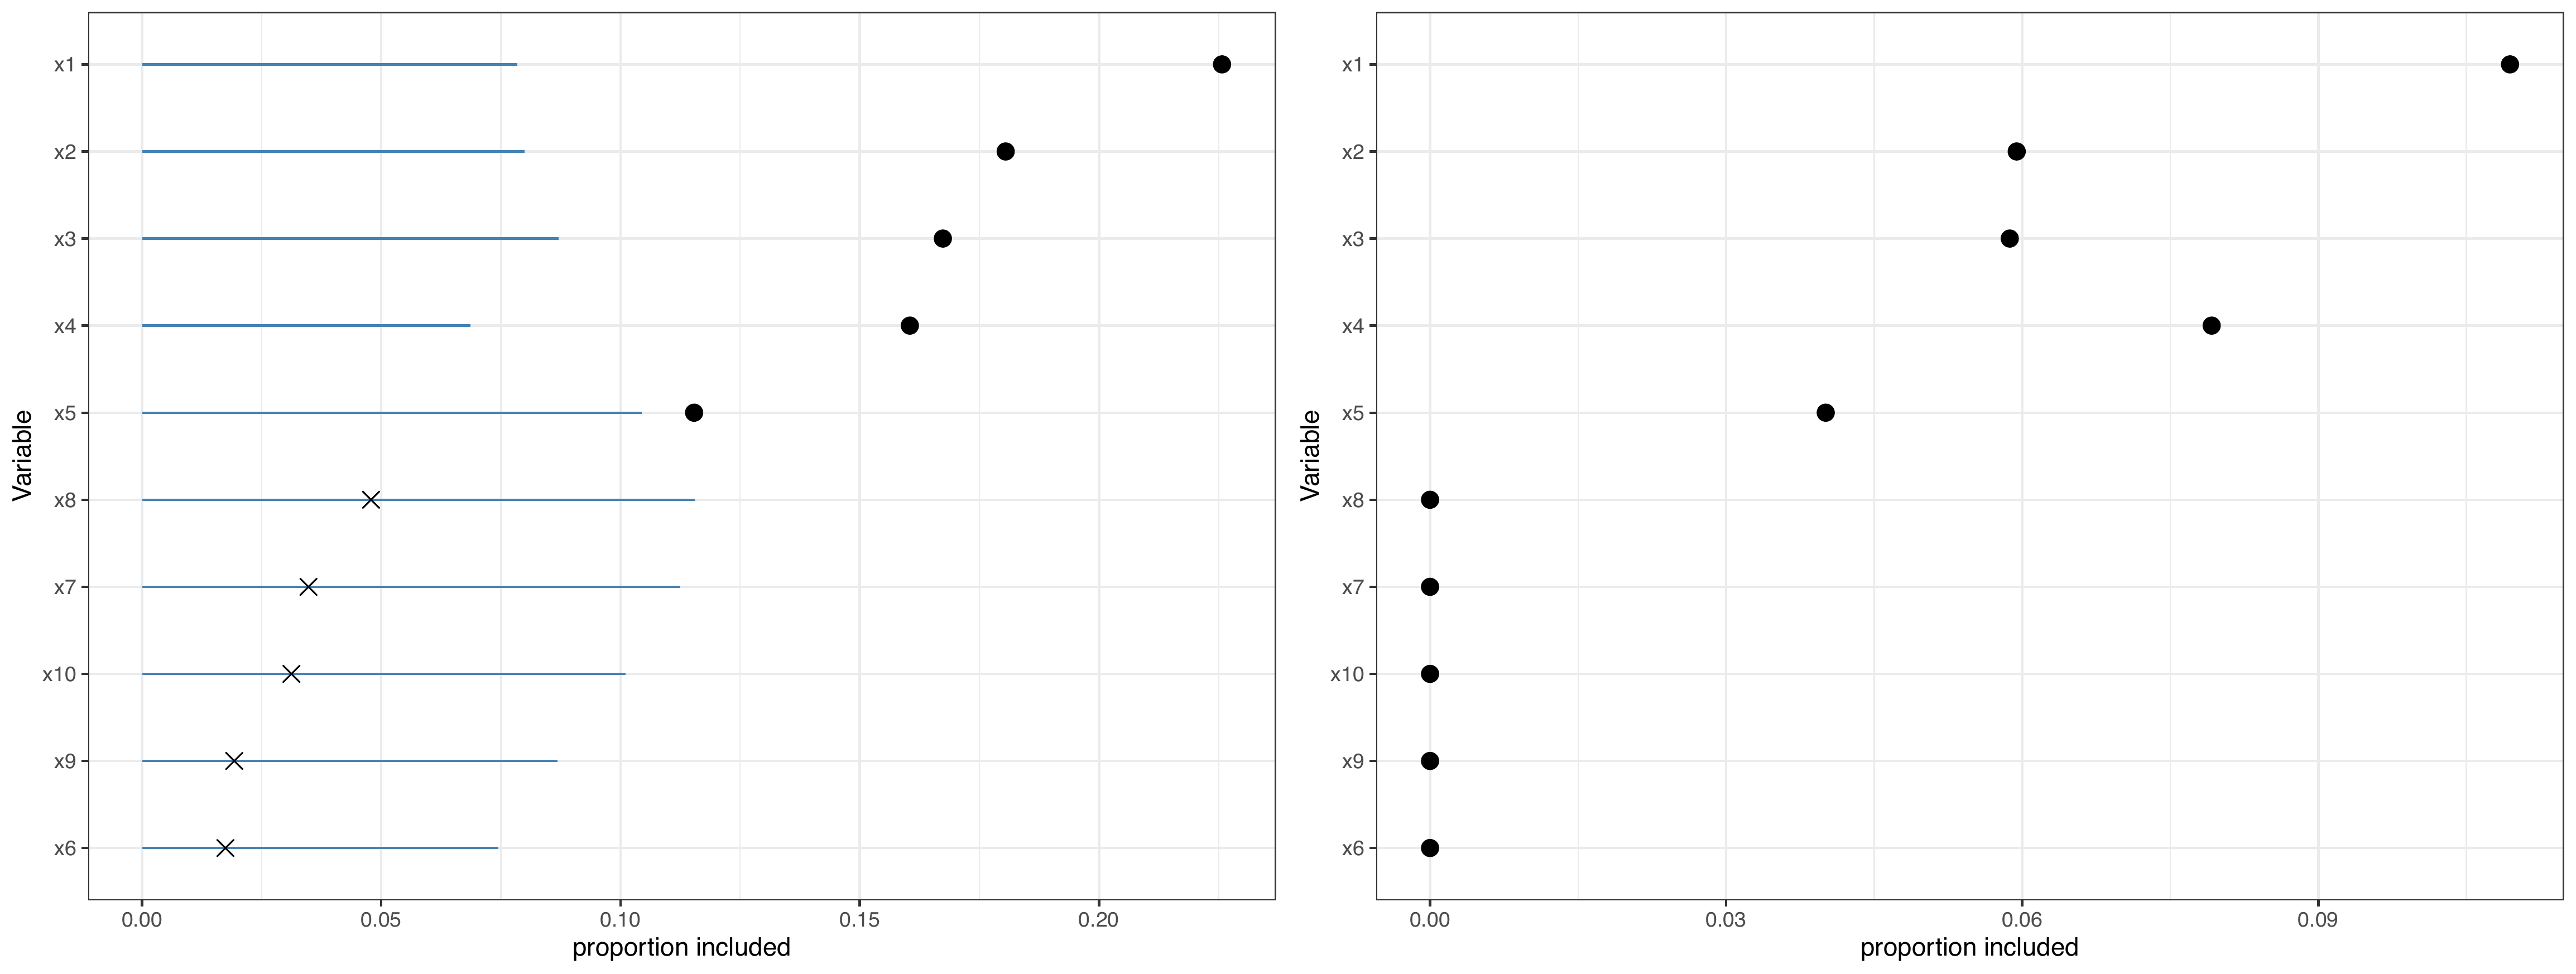
\includegraphics[width=1\linewidth]{https://github.com/AlanInglis/bartMan/blob/master/bartman_vignettte_new_plots_1/local_procedure_both.png?raw=true} \end{center}

\protect\hypertarget{fig20:fig20}{}{Figure 20: } Visualisation of the
local procedure variable selection method. The blue lines are the
threshold levels determined from the permutation distributions that must
be exceeded for a variable to be deemed important. The points are the
variable inclusion proportions for the observed data (averaged over a
selected number of duplicate BART models). If the observed value is
higher than the bar, the variable is deemed important and is displayed
as a solid dot; if not, it is displayed as an X.

\hypertarget{single-permutation-null-model}{%
\subsubsection{Single Permutation Null
Model}\label{single-permutation-null-model}}

We also provide the functionality for a variable selection approach
which creates a null model by permuting the response once, rebuilding
the model, and calculating the inclusion proportion on the null model.
The final result displayed is the original model's inclusion proportion
minus the null inclusion proportion. This function is available for both
the importance and the interactions.

\begin{Shaded}
\begin{Highlighting}[]
\FunctionTok{permVimp}\NormalTok{(}\AttributeTok{model =}\NormalTok{ dbartModel, }\AttributeTok{data =}\NormalTok{ f\_data, }\AttributeTok{response =} \StringTok{\textquotesingle{}y\textquotesingle{}}\NormalTok{,  }\AttributeTok{numTreesPerm =} \DecValTok{5}\NormalTok{)}
\FunctionTok{permVimp}\NormalTok{(}\AttributeTok{model =}\NormalTok{ dbartModel, }\AttributeTok{data =}\NormalTok{ f\_data, }\AttributeTok{response =} \StringTok{\textquotesingle{}y\textquotesingle{}}\NormalTok{,  }\AttributeTok{numTreesPerm =} \DecValTok{10}\NormalTok{)}
\FunctionTok{permVimp}\NormalTok{(}\AttributeTok{model =}\NormalTok{ dbartModel, }\AttributeTok{data =}\NormalTok{ f\_data, }\AttributeTok{response =} \StringTok{\textquotesingle{}y\textquotesingle{}}\NormalTok{,  }\AttributeTok{numTreesPerm =} \DecValTok{20}\NormalTok{)}
\end{Highlighting}
\end{Shaded}

\begin{center}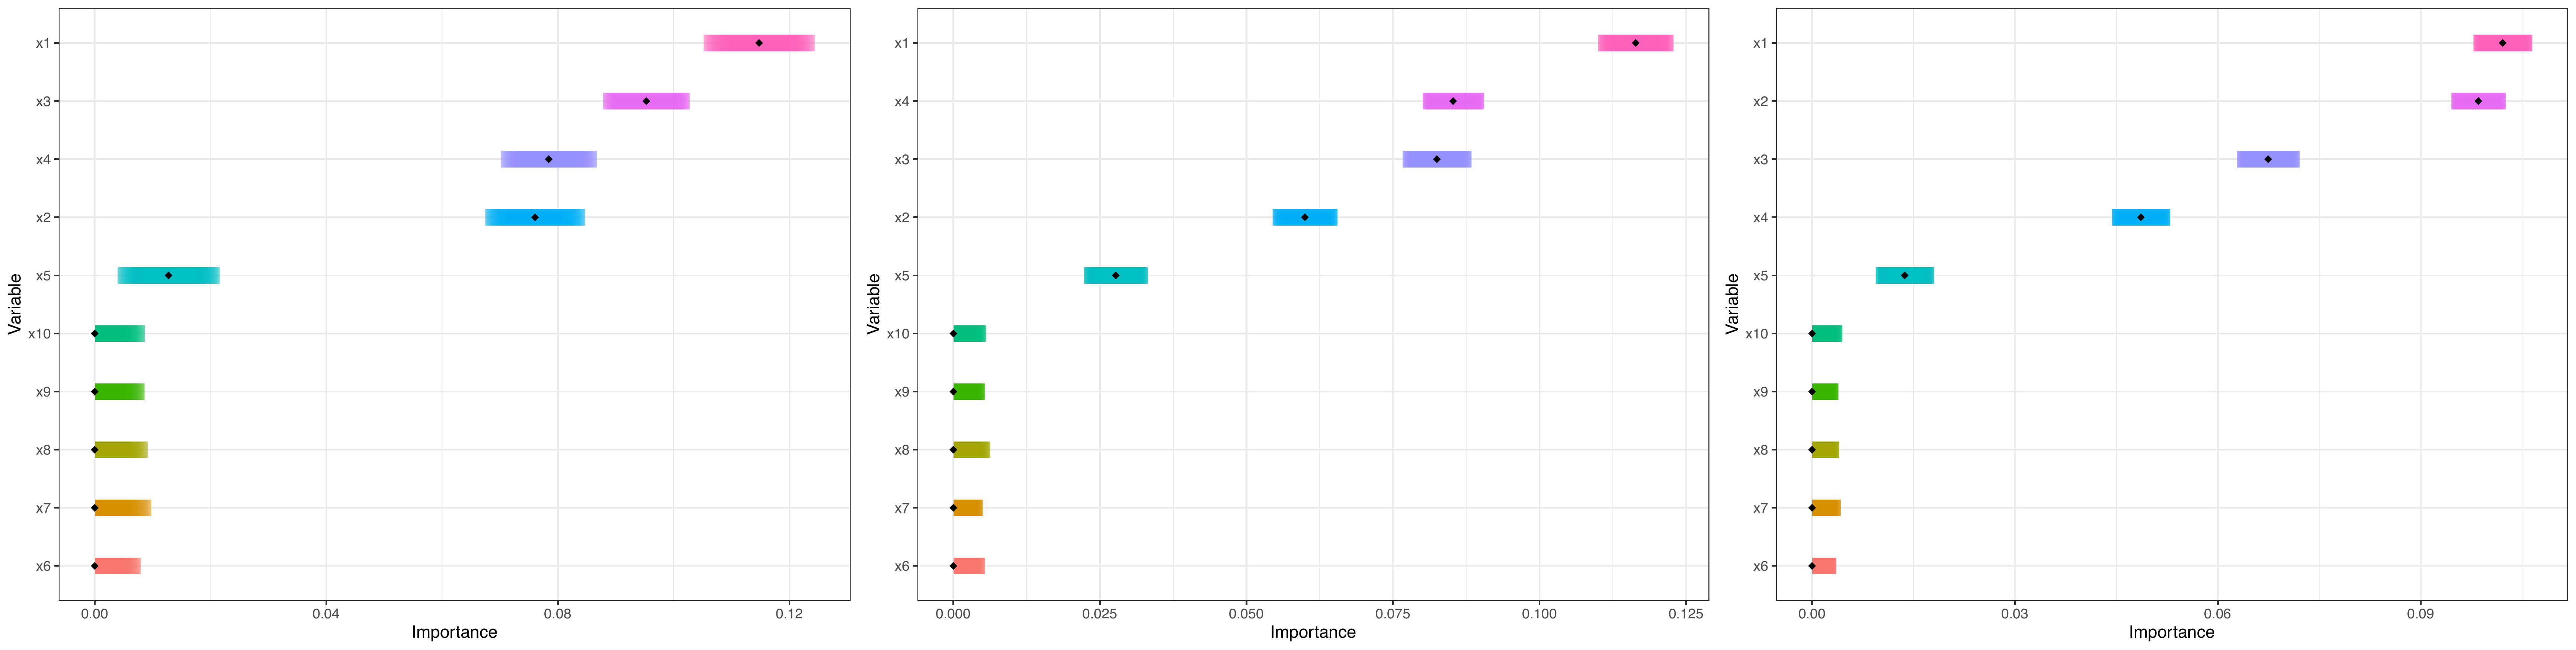
\includegraphics[width=1\linewidth]{https://github.com/AlanInglis/bartMan/blob/master/bartman_vignettte_new_plots_1/permvimp_all.png?raw=true} \end{center}

\protect\hypertarget{fig21:fig21}{}{Figure 21: } Variable importance
calculated from permuting the response and rebuilding the model. The
importance score is measured as the original model's inclusion
proportion minus the null inclusion proportion

For assessing the interactions using the single permutation method we
have:

\begin{Shaded}
\begin{Highlighting}[]
\CommentTok{\# this function is very slow}
\FunctionTok{permVint}\NormalTok{(}\AttributeTok{treeData =}\NormalTok{ trees\_data,}\AttributeTok{model =}\NormalTok{ dbartModel, }\AttributeTok{data =}\NormalTok{ f\_data, }\AttributeTok{response =} \StringTok{\textquotesingle{}y\textquotesingle{}}\NormalTok{, }\AttributeTok{top =} \DecValTok{5}\NormalTok{)}
\end{Highlighting}
\end{Shaded}

\begin{center}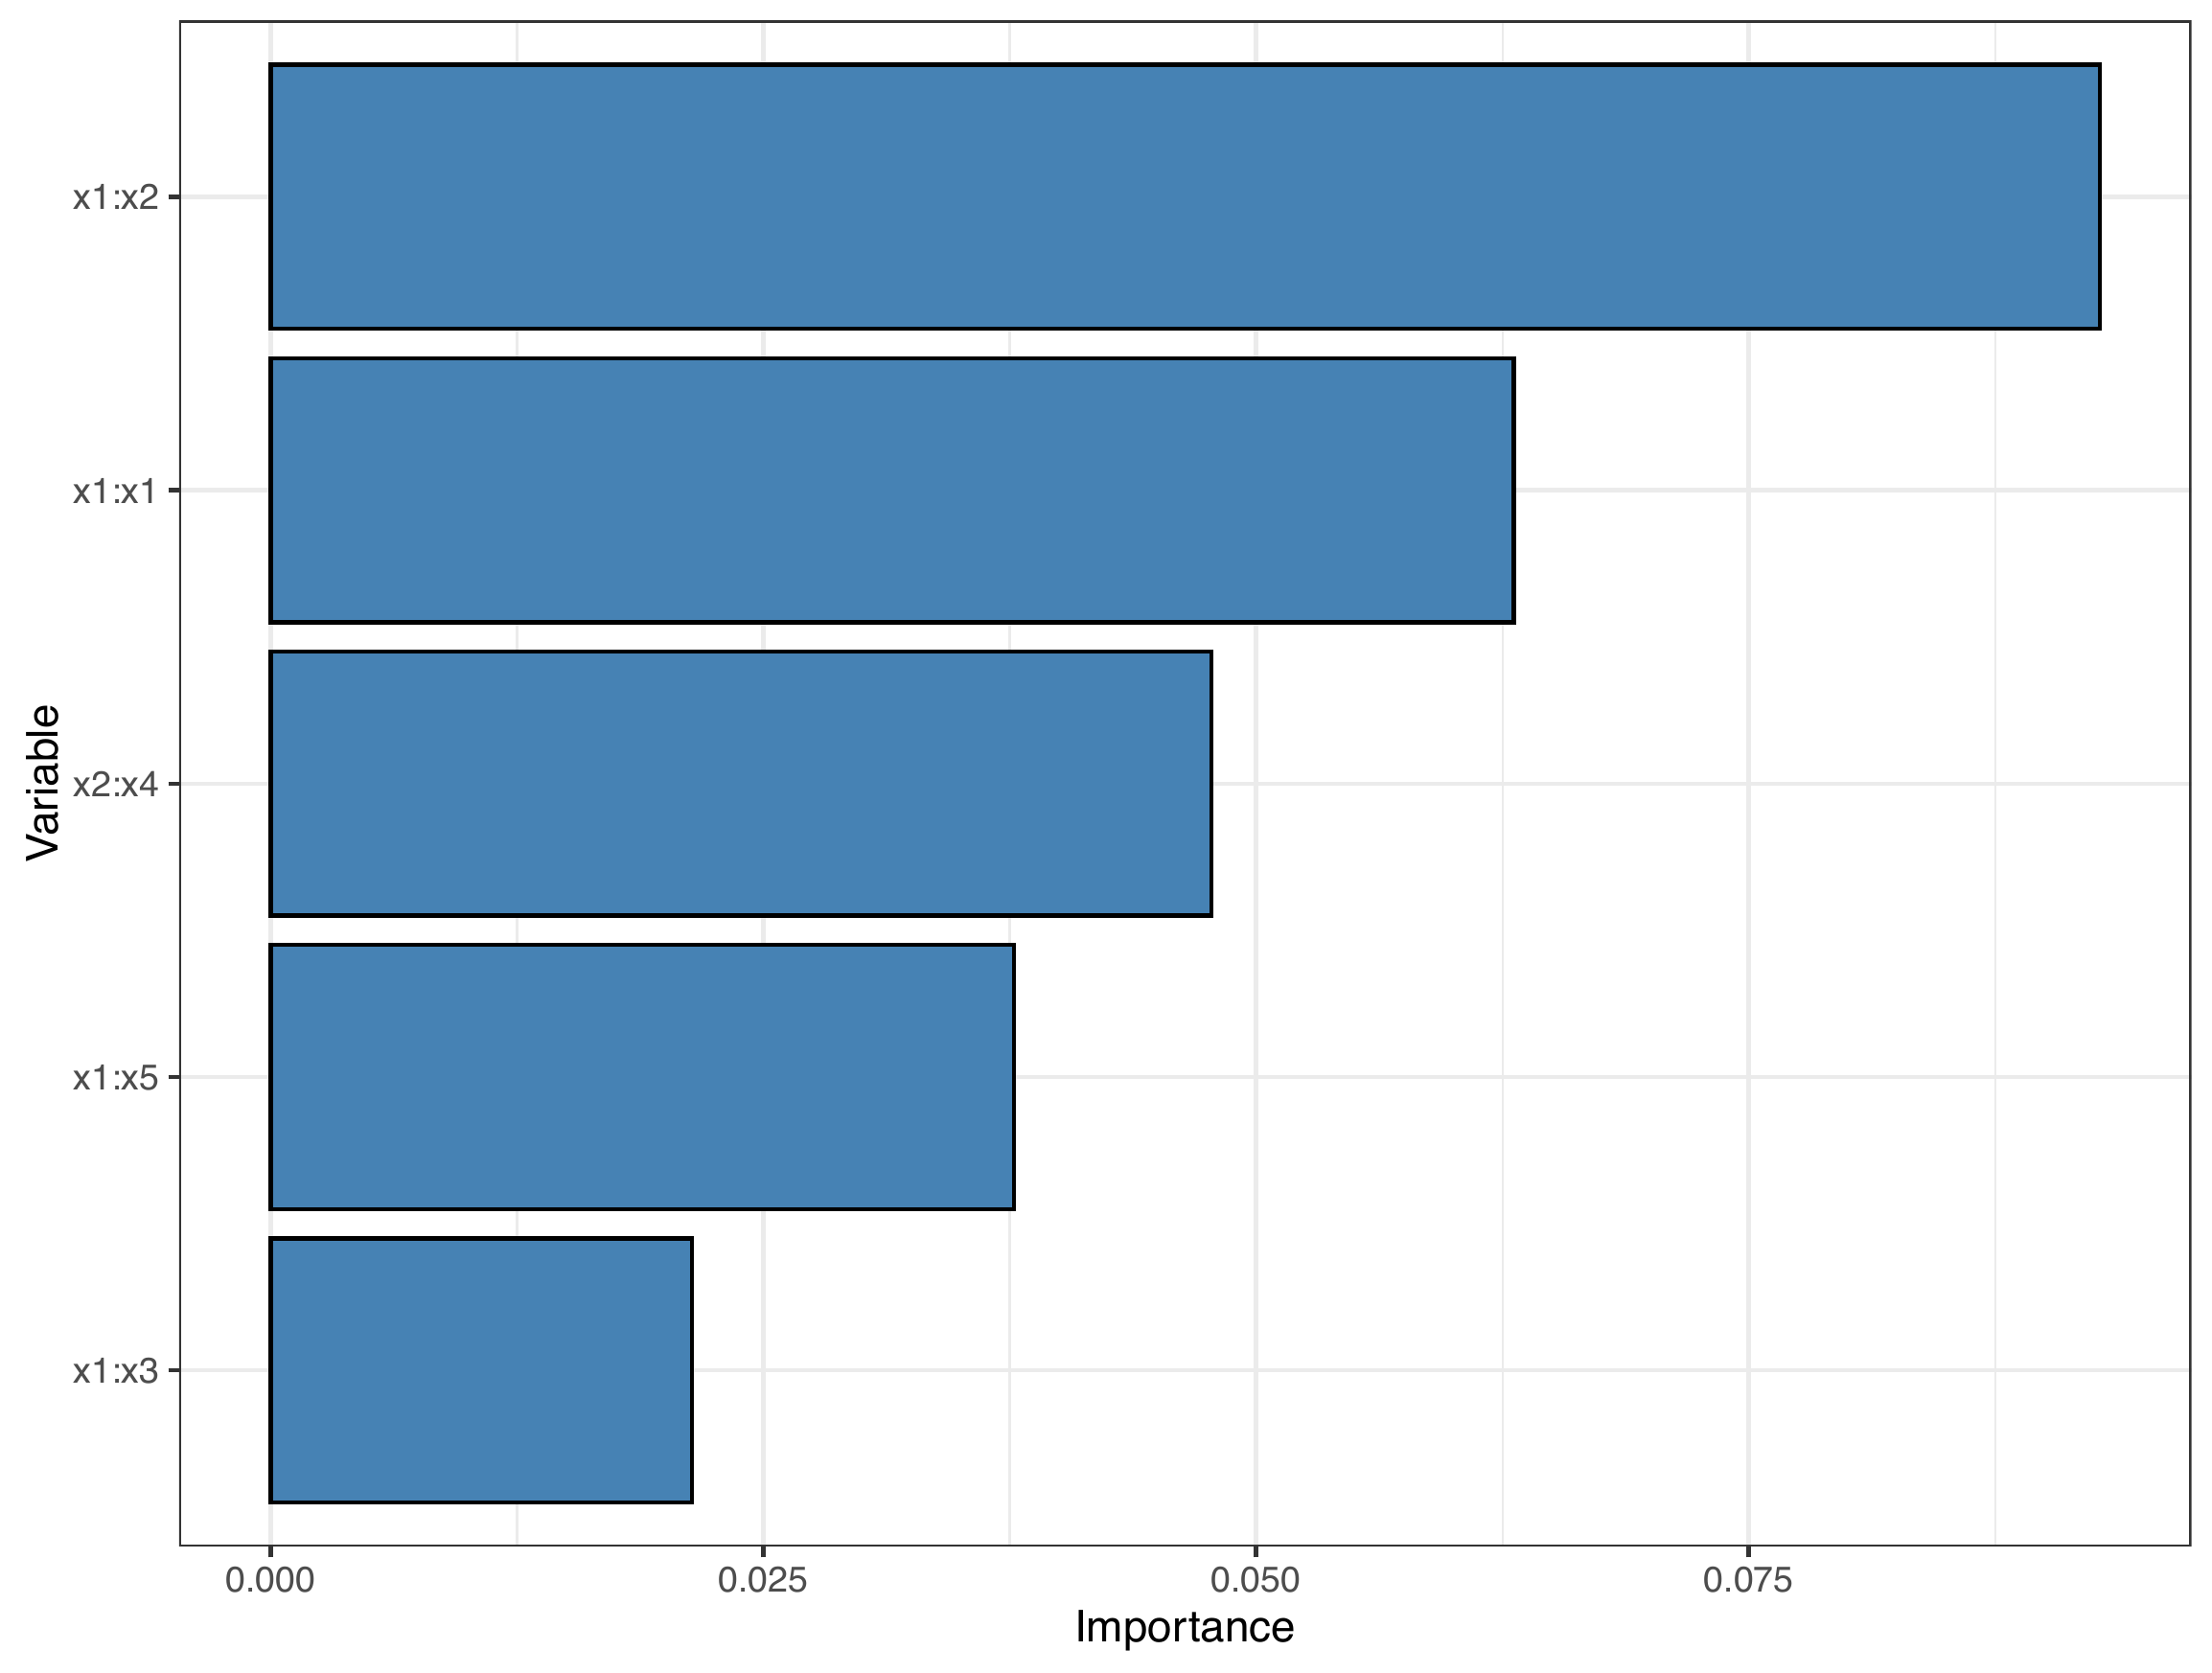
\includegraphics[width=0.6\linewidth]{https://github.com/AlanInglis/bartMan/blob/master/bartman_vignettte_new_plots_1/permvint_1.png?raw=true} \end{center}

\protect\hypertarget{fig22:fig22}{}{Figure 22: } Variable interactions
calculated from permuting the response and rebuilding the model. The
interaction score is measured as the original model's inclusion
proportion minus the null inclusion proportion

\hypertarget{utility-functions}{%
\section{Utility Functions}\label{utility-functions}}

\hypertarget{tree-list}{%
\subsection{Tree List}\label{tree-list}}

In addition to the data frame of trees, we also provide an option for
separating the trees into a list, where each element is a
\texttt{tidygraph} object, containing the structure of every individual
tree. This allows a user to quickly access each tree for custom data
analysis or visualisation, with options for selection either a specific
iteration, tree number, or both together. Each \texttt{tidygraph} object
includes node and edge information. For example, if we want to create a
list of the trees used in the first iteration, we would do the
following:

\begin{Shaded}
\begin{Highlighting}[]
\NormalTok{tree\_list }\OtherTok{\textless{}{-}} \FunctionTok{treeList}\NormalTok{(}\AttributeTok{treeData =}\NormalTok{ trees\_data, }\AttributeTok{iter =} \DecValTok{1}\NormalTok{, }\AttributeTok{treeNo =} \ConstantTok{NULL}\NormalTok{)}
\CommentTok{\#\textgreater{} Iteration 1 Selected.}
\end{Highlighting}
\end{Shaded}

Examine the first tree yields:

\begin{Shaded}
\begin{Highlighting}[]
\NormalTok{tree\_list[[}\DecValTok{1}\NormalTok{]]}
\CommentTok{\#\textgreater{} \# A tbl\_graph: 3 nodes and 2 edges}
\CommentTok{\#\textgreater{} \#}
\CommentTok{\#\textgreater{} \# A rooted tree}
\CommentTok{\#\textgreater{} \#}
\CommentTok{\#\textgreater{} \# A tibble: 3 x 11}
\CommentTok{\#\textgreater{}   var    node iteration treeNum label         value depthMax noObs respNode}
\CommentTok{\#\textgreater{}   \textless{}chr\textgreater{} \textless{}int\textgreater{}     \textless{}int\textgreater{}   \textless{}int\textgreater{} \textless{}chr\textgreater{}         \textless{}dbl\textgreater{}    \textless{}dbl\textgreater{} \textless{}int\textgreater{}    \textless{}dbl\textgreater{}}
\CommentTok{\#\textgreater{} 1 x1        1         1       1 x1  ≤  0.56  0.564         1   200    100. }
\CommentTok{\#\textgreater{} 2 \textless{}NA\textgreater{}      2         1       1 {-}0.02       {-}0.0209        1   107     99.8}
\CommentTok{\#\textgreater{} 3 \textless{}NA\textgreater{}      3         1       1 0.04         0.0357        1    93    101. }
\CommentTok{\#\textgreater{}   obsNode     isStump}
\CommentTok{\#\textgreater{}   \textless{}list\textgreater{}      \textless{}lgl\textgreater{}  }
\CommentTok{\#\textgreater{} 1 \textless{}dbl [200]\textgreater{} FALSE  }
\CommentTok{\#\textgreater{} 2 \textless{}dbl [107]\textgreater{} FALSE  }
\CommentTok{\#\textgreater{} 3 \textless{}dbl [93]\textgreater{}  FALSE  }
\CommentTok{\#\textgreater{} \#}
\CommentTok{\#\textgreater{} \# A tibble: 2 x 2}
\CommentTok{\#\textgreater{}    from    to}
\CommentTok{\#\textgreater{}   \textless{}int\textgreater{} \textless{}int\textgreater{}}
\CommentTok{\#\textgreater{} 1     1     2}
\CommentTok{\#\textgreater{} 2     1     3}
\end{Highlighting}
\end{Shaded}

As we can see, it contains many of the same columns found in the data
frame of trees. Specifically, \textbf{var}, \textbf{node},
\textbf{iteration}, \textbf{treeNum}, \textbf{label}, \textbf{value},
\textbf{depthMax}, \textbf{noObs}, \textbf{respNode}, \textbf{obsNode},
\textbf{isStump}, where each of the columns has the same meaning as
outlined previously. The one exception is \textbf{respNode}, which
contains the average response value over all observations found in a
particular node.

\hypertarget{combining-categorical-variables}{%
\subsection{Combining Categorical
Variables}\label{combining-categorical-variables}}

If any of the variables used to build the BART model are categorical,
the aforementioned BART packages replace the categorical variables with
\(d\) dummy variables, where \(d\) is the number of factor levels.
However, we provide the functionality to adjust the inclusion
proportions for variable importance and interaction by aggregating over
factor levels. This provides a complete picture of the importance of a
factor, rather than that associated with individual factor levels.

In the following example, we build a BART model using the \texttt{BART}
package where one of the covariates is a factor and extract the tree
data.

\begin{Shaded}
\begin{Highlighting}[]
\FunctionTok{library}\NormalTok{(BART)}
\CommentTok{\#\textgreater{} Loading required package: nlme}
\CommentTok{\#\textgreater{} Loading required package: nnet}
\CommentTok{\#\textgreater{} Loading required package: survival}

\FunctionTok{data}\NormalTok{(iris)}
\FunctionTok{set.seed}\NormalTok{(}\DecValTok{1701}\NormalTok{)}
\NormalTok{bartModel }\OtherTok{\textless{}{-}} \FunctionTok{wbart}\NormalTok{(}\AttributeTok{x.train =}\NormalTok{ iris[,}\DecValTok{2}\SpecialCharTok{:}\DecValTok{5}\NormalTok{],}
                   \AttributeTok{y.train =}\NormalTok{ iris[,}\DecValTok{1}\NormalTok{],}
                   \AttributeTok{nskip =} \DecValTok{10}\NormalTok{,}
                   \AttributeTok{ndpost =} \DecValTok{100}\NormalTok{,}
                   \AttributeTok{nkeeptreedraws =} \DecValTok{100}\NormalTok{,}
                   \AttributeTok{ntree =} \DecValTok{5}
\NormalTok{)}

\NormalTok{btt }\OtherTok{\textless{}{-}} \FunctionTok{extractTreeData}\NormalTok{(}\AttributeTok{model =}\NormalTok{ bartModel, }\AttributeTok{data =}\NormalTok{ iris)}
\end{Highlighting}
\end{Shaded}

As species is a factor with three levels, it is split into three dummy
variables when building the model. For a practical example of what this
looks like, we examine the variable importance inclusion proportions
both before and after aggregating over the factor levels.

\begin{Shaded}
\begin{Highlighting}[]
\CommentTok{\# extract the vimp data}
\NormalTok{vimpData }\OtherTok{\textless{}{-}} \FunctionTok{viviBart}\NormalTok{(}\AttributeTok{treeData =}\NormalTok{ btt,  }\AttributeTok{out =} \StringTok{\textquotesingle{}vimp\textquotesingle{}}\NormalTok{)}
\NormalTok{vimpData[,}\DecValTok{1}\SpecialCharTok{:}\DecValTok{3}\NormalTok{] }\CommentTok{\# looking at the relevant columns}
\CommentTok{\#\textgreater{}                  variable count   propMean}
\CommentTok{\#\textgreater{} Sepal.Width   Sepal.Width   234 0.23382715}
\CommentTok{\#\textgreater{} Petal.Length Petal.Length   416 0.40474595}
\CommentTok{\#\textgreater{} Petal.Width   Petal.Width   181 0.19423754}
\CommentTok{\#\textgreater{} Species1         Species1    95 0.09627939}
\CommentTok{\#\textgreater{} Species2         Species2    32 0.02590565}
\CommentTok{\#\textgreater{} Species3         Species3    38 0.04500433}
\end{Highlighting}
\end{Shaded}

Combine variables

\begin{Shaded}
\begin{Highlighting}[]
\NormalTok{btt\_combined }\OtherTok{\textless{}{-}} \FunctionTok{combineDummy}\NormalTok{(}\AttributeTok{trees =}\NormalTok{ btt)}
\end{Highlighting}
\end{Shaded}

looking again we see the dummies are combined

\begin{Shaded}
\begin{Highlighting}[]
\CommentTok{\# extract the vimp data}
\NormalTok{vimpData\_combined }\OtherTok{\textless{}{-}} \FunctionTok{viviBart}\NormalTok{(}\AttributeTok{treeData =}\NormalTok{ btt\_combined,  }\AttributeTok{out =} \StringTok{\textquotesingle{}vimp\textquotesingle{}}\NormalTok{)}
\NormalTok{vimpData\_combined[,}\DecValTok{1}\SpecialCharTok{:}\DecValTok{3}\NormalTok{] }\CommentTok{\# looking at the relevant columns}
\CommentTok{\#\textgreater{}                  variable count  propMean}
\CommentTok{\#\textgreater{} Sepal.Length Sepal.Length     0 0.0000000}
\CommentTok{\#\textgreater{} Sepal.Width   Sepal.Width   234 0.2338271}
\CommentTok{\#\textgreater{} Petal.Length Petal.Length   416 0.4047459}
\CommentTok{\#\textgreater{} Petal.Width   Petal.Width   181 0.1942375}
\CommentTok{\#\textgreater{} Species           Species   165 0.1671894}
\end{Highlighting}
\end{Shaded}

taking a look at the trees before and after combining the dummy
variables

\begin{Shaded}
\begin{Highlighting}[]
\FunctionTok{plotTrees}\NormalTok{(}\AttributeTok{trees =}\NormalTok{ btt, }\AttributeTok{iter =} \DecValTok{1}\NormalTok{)}
\FunctionTok{plotTrees}\NormalTok{(}\AttributeTok{trees =}\NormalTok{ btt\_combined, }\AttributeTok{iter =} \DecValTok{1}\NormalTok{)}
\end{Highlighting}
\end{Shaded}

\begin{center}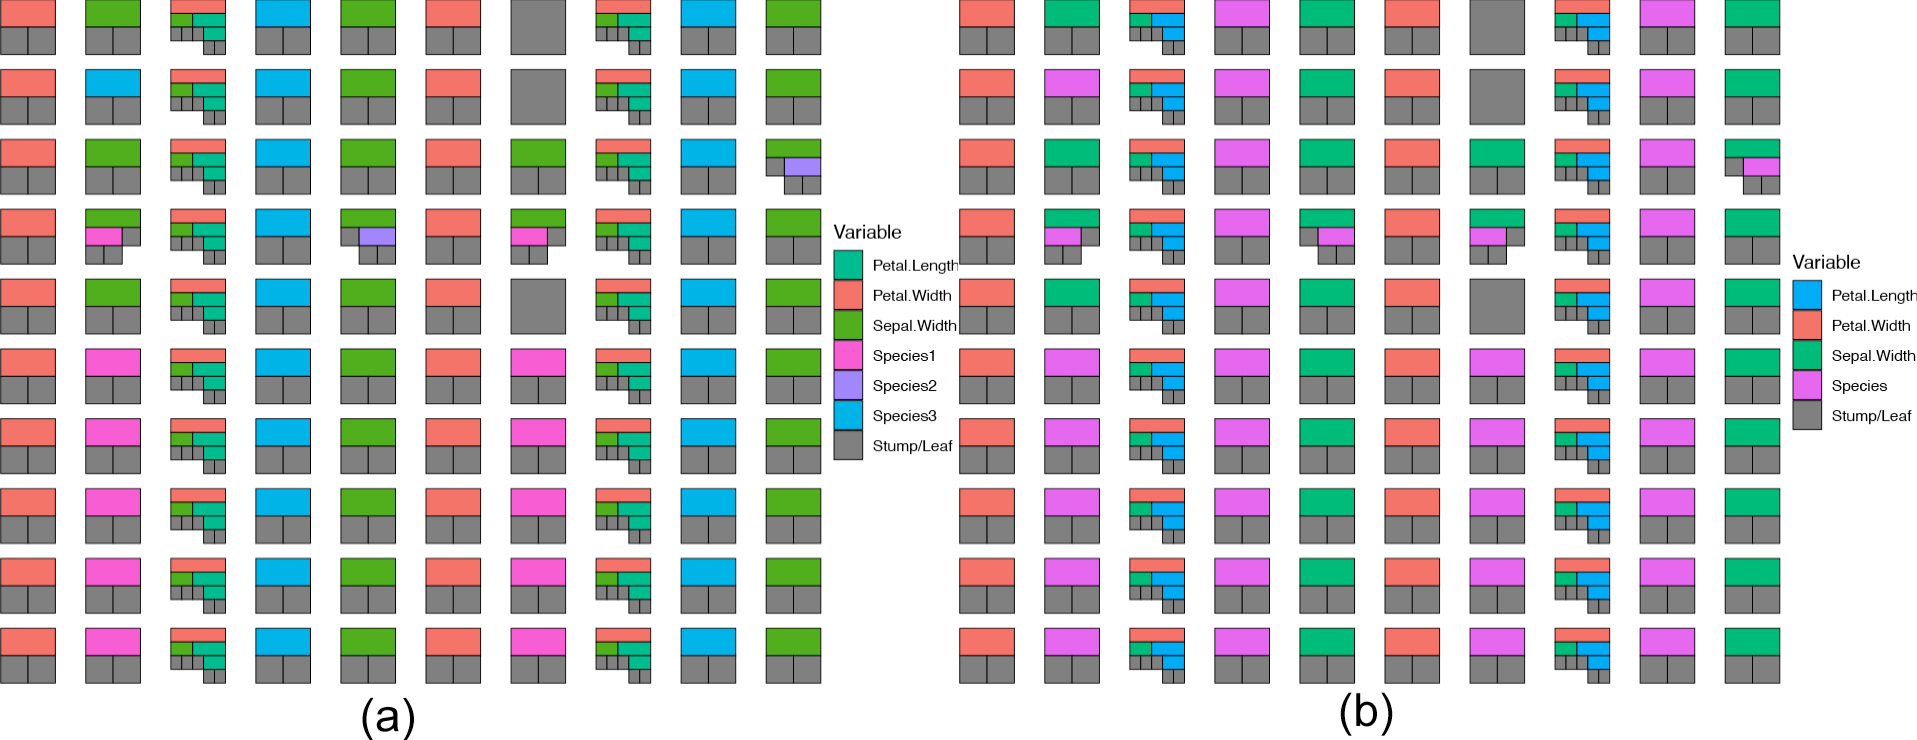
\includegraphics[width=1\linewidth]{https://github.com/AlanInglis/bartMan/blob/master/bartman_vignettte_new_plots_1/trees_dummy_1.png?raw=true} \end{center}

\protect\hypertarget{fig23:fig23}{}{Figure 23: }stuff here!!!!!

\hypertarget{creating-your-own-data-frame-of-trees-to-plot}{%
\subsection{Creating Your Own Data Frame Of Trees To
Plot}\label{creating-your-own-data-frame-of-trees-to-plot}}

STUFF HERE!!

\begin{Shaded}
\begin{Highlighting}[]

\CommentTok{\# Original Data}
\NormalTok{f\_data }\OtherTok{\textless{}{-}} \FunctionTok{data.frame}\NormalTok{(}
  \AttributeTok{x1 =} \FunctionTok{c}\NormalTok{(}\FloatTok{0.127393428}\NormalTok{, }\FloatTok{0.766723202}\NormalTok{, }\FloatTok{0.054421675}\NormalTok{, }\FloatTok{0.561384595}\NormalTok{, }\FloatTok{0.937597936}\NormalTok{,}
         \FloatTok{0.296445079}\NormalTok{, }\FloatTok{0.665117463}\NormalTok{, }\FloatTok{0.652215607}\NormalTok{, }\FloatTok{0.002313313}\NormalTok{, }\FloatTok{0.661490602}\NormalTok{),}
  \AttributeTok{x2 =} \FunctionTok{c}\NormalTok{(}\FloatTok{0.85600486}\NormalTok{, }\FloatTok{0.02407293}\NormalTok{, }\FloatTok{0.51942589}\NormalTok{, }\FloatTok{0.20590965}\NormalTok{, }\FloatTok{0.71206404}\NormalTok{,}
         \FloatTok{0.27272126}\NormalTok{, }\FloatTok{0.66765977}\NormalTok{, }\FloatTok{0.94837341}\NormalTok{, }\FloatTok{0.46710461}\NormalTok{, }\FloatTok{0.84157353}\NormalTok{),}
  \AttributeTok{x3 =} \FunctionTok{c}\NormalTok{(}\FloatTok{0.4791849}\NormalTok{, }\FloatTok{0.8265008}\NormalTok{, }\FloatTok{0.1076198}\NormalTok{, }\FloatTok{0.2213454}\NormalTok{, }\FloatTok{0.6717478}\NormalTok{,}
         \FloatTok{0.5053170}\NormalTok{, }\FloatTok{0.8849426}\NormalTok{, }\FloatTok{0.3560469}\NormalTok{, }\FloatTok{0.5732139}\NormalTok{, }\FloatTok{0.5091688}\NormalTok{),}
  \AttributeTok{x4 =} \FunctionTok{c}\NormalTok{(}\FloatTok{0.55089910}\NormalTok{, }\FloatTok{0.35612092}\NormalTok{, }\FloatTok{0.80230714}\NormalTok{, }\FloatTok{0.73043828}\NormalTok{, }\FloatTok{0.72341749}\NormalTok{,}
         \FloatTok{0.98789408}\NormalTok{, }\FloatTok{0.04751297}\NormalTok{, }\FloatTok{0.06630861}\NormalTok{, }\FloatTok{0.55040341}\NormalTok{, }\FloatTok{0.95719901}\NormalTok{),}
  \AttributeTok{x5 =} \FunctionTok{c}\NormalTok{(}\FloatTok{0.9201376}\NormalTok{, }\FloatTok{0.9279873}\NormalTok{, }\FloatTok{0.5993939}\NormalTok{, }\FloatTok{0.1135139}\NormalTok{, }\FloatTok{0.2472984}\NormalTok{,}
         \FloatTok{0.4514940}\NormalTok{, }\FloatTok{0.3097986}\NormalTok{, }\FloatTok{0.2608917}\NormalTok{, }\FloatTok{0.5375610}\NormalTok{, }\FloatTok{0.9608329}\NormalTok{),}
  \AttributeTok{y =} \FunctionTok{c}\NormalTok{(}\FloatTok{14.318655}\NormalTok{, }\FloatTok{12.052513}\NormalTok{, }\FloatTok{13.689970}\NormalTok{, }\FloatTok{13.433919}\NormalTok{, }\FloatTok{18.542184}\NormalTok{,}
        \FloatTok{14.927344}\NormalTok{, }\FloatTok{14.843248}\NormalTok{, }\FloatTok{13.611167}\NormalTok{, }\FloatTok{7.777591}\NormalTok{, }\FloatTok{23.895456}\NormalTok{)}
\NormalTok{  )}


\CommentTok{\# Your own data frame of trees}
\NormalTok{df\_tree }\OtherTok{\textless{}{-}} \FunctionTok{data.frame}\NormalTok{(}
  \AttributeTok{var =} \FunctionTok{c}\NormalTok{(}\StringTok{"x3"}\NormalTok{, }\StringTok{"x1"}\NormalTok{, }\ConstantTok{NA}\NormalTok{, }\ConstantTok{NA}\NormalTok{, }\ConstantTok{NA}\NormalTok{, }\StringTok{"x1"}\NormalTok{, }\ConstantTok{NA}\NormalTok{, }\ConstantTok{NA}\NormalTok{, }\StringTok{"x3"}\NormalTok{, }\ConstantTok{NA}\NormalTok{, }\ConstantTok{NA}\NormalTok{, }\StringTok{"x1"}\NormalTok{, }\ConstantTok{NA}\NormalTok{, }\ConstantTok{NA}\NormalTok{),}
  \AttributeTok{value =} \FunctionTok{c}\NormalTok{(}\FloatTok{0.823}\NormalTok{,}\FloatTok{0.771}\NormalTok{,}\SpecialCharTok{{-}}\FloatTok{0.0433}\NormalTok{,}\FloatTok{0.0188}\NormalTok{,}\SpecialCharTok{{-}}\FloatTok{0.252}\NormalTok{,}\FloatTok{0.215}\NormalTok{,}\SpecialCharTok{{-}}\FloatTok{0.269}\NormalTok{,}\FloatTok{0.117}\NormalTok{,}\FloatTok{0.823}\NormalTok{,}\FloatTok{0.0036}\NormalTok{,}\SpecialCharTok{{-}}\FloatTok{0.244}\NormalTok{,}\FloatTok{0.215}\NormalTok{,}\SpecialCharTok{{-}}\FloatTok{0.222}\NormalTok{,}\FloatTok{0.0783}\NormalTok{),}
  \AttributeTok{iteration =} \FunctionTok{c}\NormalTok{(}\DecValTok{1}\NormalTok{, }\DecValTok{1}\NormalTok{, }\DecValTok{1}\NormalTok{, }\DecValTok{1}\NormalTok{, }\DecValTok{1}\NormalTok{, }\DecValTok{1}\NormalTok{, }\DecValTok{1}\NormalTok{, }\DecValTok{1}\NormalTok{, }\DecValTok{2}\NormalTok{, }\DecValTok{2}\NormalTok{, }\DecValTok{2}\NormalTok{, }\DecValTok{2}\NormalTok{, }\DecValTok{2}\NormalTok{, }\DecValTok{2}\NormalTok{),}
  \AttributeTok{treeNum =} \FunctionTok{c}\NormalTok{(}\DecValTok{1}\NormalTok{, }\DecValTok{1}\NormalTok{, }\DecValTok{1}\NormalTok{, }\DecValTok{1}\NormalTok{, }\DecValTok{1}\NormalTok{, }\DecValTok{2}\NormalTok{, }\DecValTok{2}\NormalTok{, }\DecValTok{2}\NormalTok{, }\DecValTok{1}\NormalTok{, }\DecValTok{1}\NormalTok{, }\DecValTok{1}\NormalTok{, }\DecValTok{2}\NormalTok{, }\DecValTok{2}\NormalTok{, }\DecValTok{2}\NormalTok{)}
\NormalTok{)}

\NormalTok{df\_tree}
\CommentTok{\#\textgreater{}     var   value iteration treeNum}
\CommentTok{\#\textgreater{} 1    x3  0.8230         1       1}
\CommentTok{\#\textgreater{} 2    x1  0.7710         1       1}
\CommentTok{\#\textgreater{} 3  \textless{}NA\textgreater{} {-}0.0433         1       1}
\CommentTok{\#\textgreater{} 4  \textless{}NA\textgreater{}  0.0188         1       1}
\CommentTok{\#\textgreater{} 5  \textless{}NA\textgreater{} {-}0.2520         1       1}
\CommentTok{\#\textgreater{} 6    x1  0.2150         1       2}
\CommentTok{\#\textgreater{} 7  \textless{}NA\textgreater{} {-}0.2690         1       2}
\CommentTok{\#\textgreater{} 8  \textless{}NA\textgreater{}  0.1170         1       2}
\CommentTok{\#\textgreater{} 9    x3  0.8230         2       1}
\CommentTok{\#\textgreater{} 10 \textless{}NA\textgreater{}  0.0036         2       1}
\CommentTok{\#\textgreater{} 11 \textless{}NA\textgreater{} {-}0.2440         2       1}
\CommentTok{\#\textgreater{} 12   x1  0.2150         2       2}
\CommentTok{\#\textgreater{} 13 \textless{}NA\textgreater{} {-}0.2220         2       2}
\CommentTok{\#\textgreater{} 14 \textless{}NA\textgreater{}  0.0783         2       2}
\end{Highlighting}
\end{Shaded}

\begin{Shaded}
\begin{Highlighting}[]
\NormalTok{trees\_data }\OtherTok{\textless{}{-}} \FunctionTok{tree\_dataframe}\NormalTok{(}\AttributeTok{data =}\NormalTok{ f\_data , }\AttributeTok{trees =}\NormalTok{ df\_tree)}
\end{Highlighting}
\end{Shaded}

\begin{Shaded}
\begin{Highlighting}[]
\NormalTok{trees\_data}
\CommentTok{\#\textgreater{} Tree dataframe:}
\CommentTok{\#\textgreater{} \# A tibble: 14 x 17}
\CommentTok{\#\textgreater{}    var   splitValue terminal leafValue iteration treeNum  node childLeft}
\CommentTok{\#\textgreater{}    \textless{}chr\textgreater{}      \textless{}dbl\textgreater{} \textless{}lgl\textgreater{}        \textless{}dbl\textgreater{}     \textless{}dbl\textgreater{}   \textless{}dbl\textgreater{} \textless{}int\textgreater{}     \textless{}int\textgreater{}}
\CommentTok{\#\textgreater{}  1 x3         0.823 FALSE      NA              1       1     1         2}
\CommentTok{\#\textgreater{}  2 x1         0.771 FALSE      NA              1       1     2         3}
\CommentTok{\#\textgreater{}  3 \textless{}NA\textgreater{}      NA     TRUE       {-}0.0433         1       1     3        NA}
\CommentTok{\#\textgreater{}  4 \textless{}NA\textgreater{}      NA     TRUE        0.0188         1       1     4        NA}
\CommentTok{\#\textgreater{}  5 \textless{}NA\textgreater{}      NA     TRUE       {-}0.252          1       1     5        NA}
\CommentTok{\#\textgreater{}  6 x1         0.215 FALSE      NA              1       2     1         2}
\CommentTok{\#\textgreater{}  7 \textless{}NA\textgreater{}      NA     TRUE       {-}0.269          1       2     2        NA}
\CommentTok{\#\textgreater{}  8 \textless{}NA\textgreater{}      NA     TRUE        0.117          1       2     3        NA}
\CommentTok{\#\textgreater{}  9 x3         0.823 FALSE      NA              2       1     1         2}
\CommentTok{\#\textgreater{} 10 \textless{}NA\textgreater{}      NA     TRUE        0.0036         2       1     2        NA}
\CommentTok{\#\textgreater{} 11 \textless{}NA\textgreater{}      NA     TRUE       {-}0.244          2       1     3        NA}
\CommentTok{\#\textgreater{} 12 x1         0.215 FALSE      NA              2       2     1         2}
\CommentTok{\#\textgreater{} 13 \textless{}NA\textgreater{}      NA     TRUE       {-}0.222          2       2     2        NA}
\CommentTok{\#\textgreater{} 14 \textless{}NA\textgreater{}      NA     TRUE        0.0783         2       2     3        NA}
\CommentTok{\#\textgreater{}    childRight parent depth depthMax isStump label         value obsNode    noObs}
\CommentTok{\#\textgreater{}         \textless{}int\textgreater{}  \textless{}int\textgreater{} \textless{}dbl\textgreater{}    \textless{}dbl\textgreater{} \textless{}lgl\textgreater{}   \textless{}chr\textgreater{}         \textless{}dbl\textgreater{} \textless{}list\textgreater{}     \textless{}int\textgreater{}}
\CommentTok{\#\textgreater{}  1          5     NA     0        2 FALSE   x3  ≤  0.82  0.823  \textless{}dbl [10]\textgreater{}    10}
\CommentTok{\#\textgreater{}  2          4      1     1        2 FALSE   x1  ≤  0.77  0.771  \textless{}dbl [8]\textgreater{}      8}
\CommentTok{\#\textgreater{}  3         NA      2     2        2 FALSE   {-}0.04       {-}0.0433 \textless{}dbl [7]\textgreater{}      7}
\CommentTok{\#\textgreater{}  4         NA      2     2        2 FALSE   0.02         0.0188 \textless{}dbl [1]\textgreater{}      1}
\CommentTok{\#\textgreater{}  5         NA      1     1        2 FALSE   {-}0.25       {-}0.252  \textless{}dbl [2]\textgreater{}      2}
\CommentTok{\#\textgreater{}  6          3     NA     0        1 FALSE   x1  ≤  0.22  0.215  \textless{}dbl [10]\textgreater{}    10}
\CommentTok{\#\textgreater{}  7         NA      1     1        1 FALSE   {-}0.27       {-}0.269  \textless{}dbl [3]\textgreater{}      3}
\CommentTok{\#\textgreater{}  8         NA      1     1        1 FALSE   0.12         0.117  \textless{}dbl [7]\textgreater{}      7}
\CommentTok{\#\textgreater{}  9          3     NA     0        1 FALSE   x3  ≤  0.82  0.823  \textless{}dbl [10]\textgreater{}    10}
\CommentTok{\#\textgreater{} 10         NA      1     1        1 FALSE   0            0.0036 \textless{}dbl [8]\textgreater{}      8}
\CommentTok{\#\textgreater{} 11         NA      1     1        1 FALSE   {-}0.24       {-}0.244  \textless{}dbl [2]\textgreater{}      2}
\CommentTok{\#\textgreater{} 12          3     NA     0        1 FALSE   x1  ≤  0.22  0.215  \textless{}dbl [10]\textgreater{}    10}
\CommentTok{\#\textgreater{} 13         NA      1     1        1 FALSE   {-}0.22       {-}0.222  \textless{}dbl [3]\textgreater{}      3}
\CommentTok{\#\textgreater{} 14         NA      1     1        1 FALSE   0.08         0.0783 \textless{}dbl [7]\textgreater{}      7}
\CommentTok{\#\textgreater{} Variable names:}
\CommentTok{\#\textgreater{} [1] "x1" "x2" "x3" "x4" "x5" "y" }
\CommentTok{\#\textgreater{} nMCMC:}
\CommentTok{\#\textgreater{} [1] 2}
\CommentTok{\#\textgreater{} nTree:}
\CommentTok{\#\textgreater{} [1] 2}
\CommentTok{\#\textgreater{} nVar:}
\CommentTok{\#\textgreater{} [1] 6}
\end{Highlighting}
\end{Shaded}

\begin{Shaded}
\begin{Highlighting}[]
\FunctionTok{plotTrees}\NormalTok{(}\AttributeTok{trees =}\NormalTok{ trees\_data, }\AttributeTok{iter =} \ConstantTok{NULL}\NormalTok{)}
\end{Highlighting}
\end{Shaded}

\begin{center}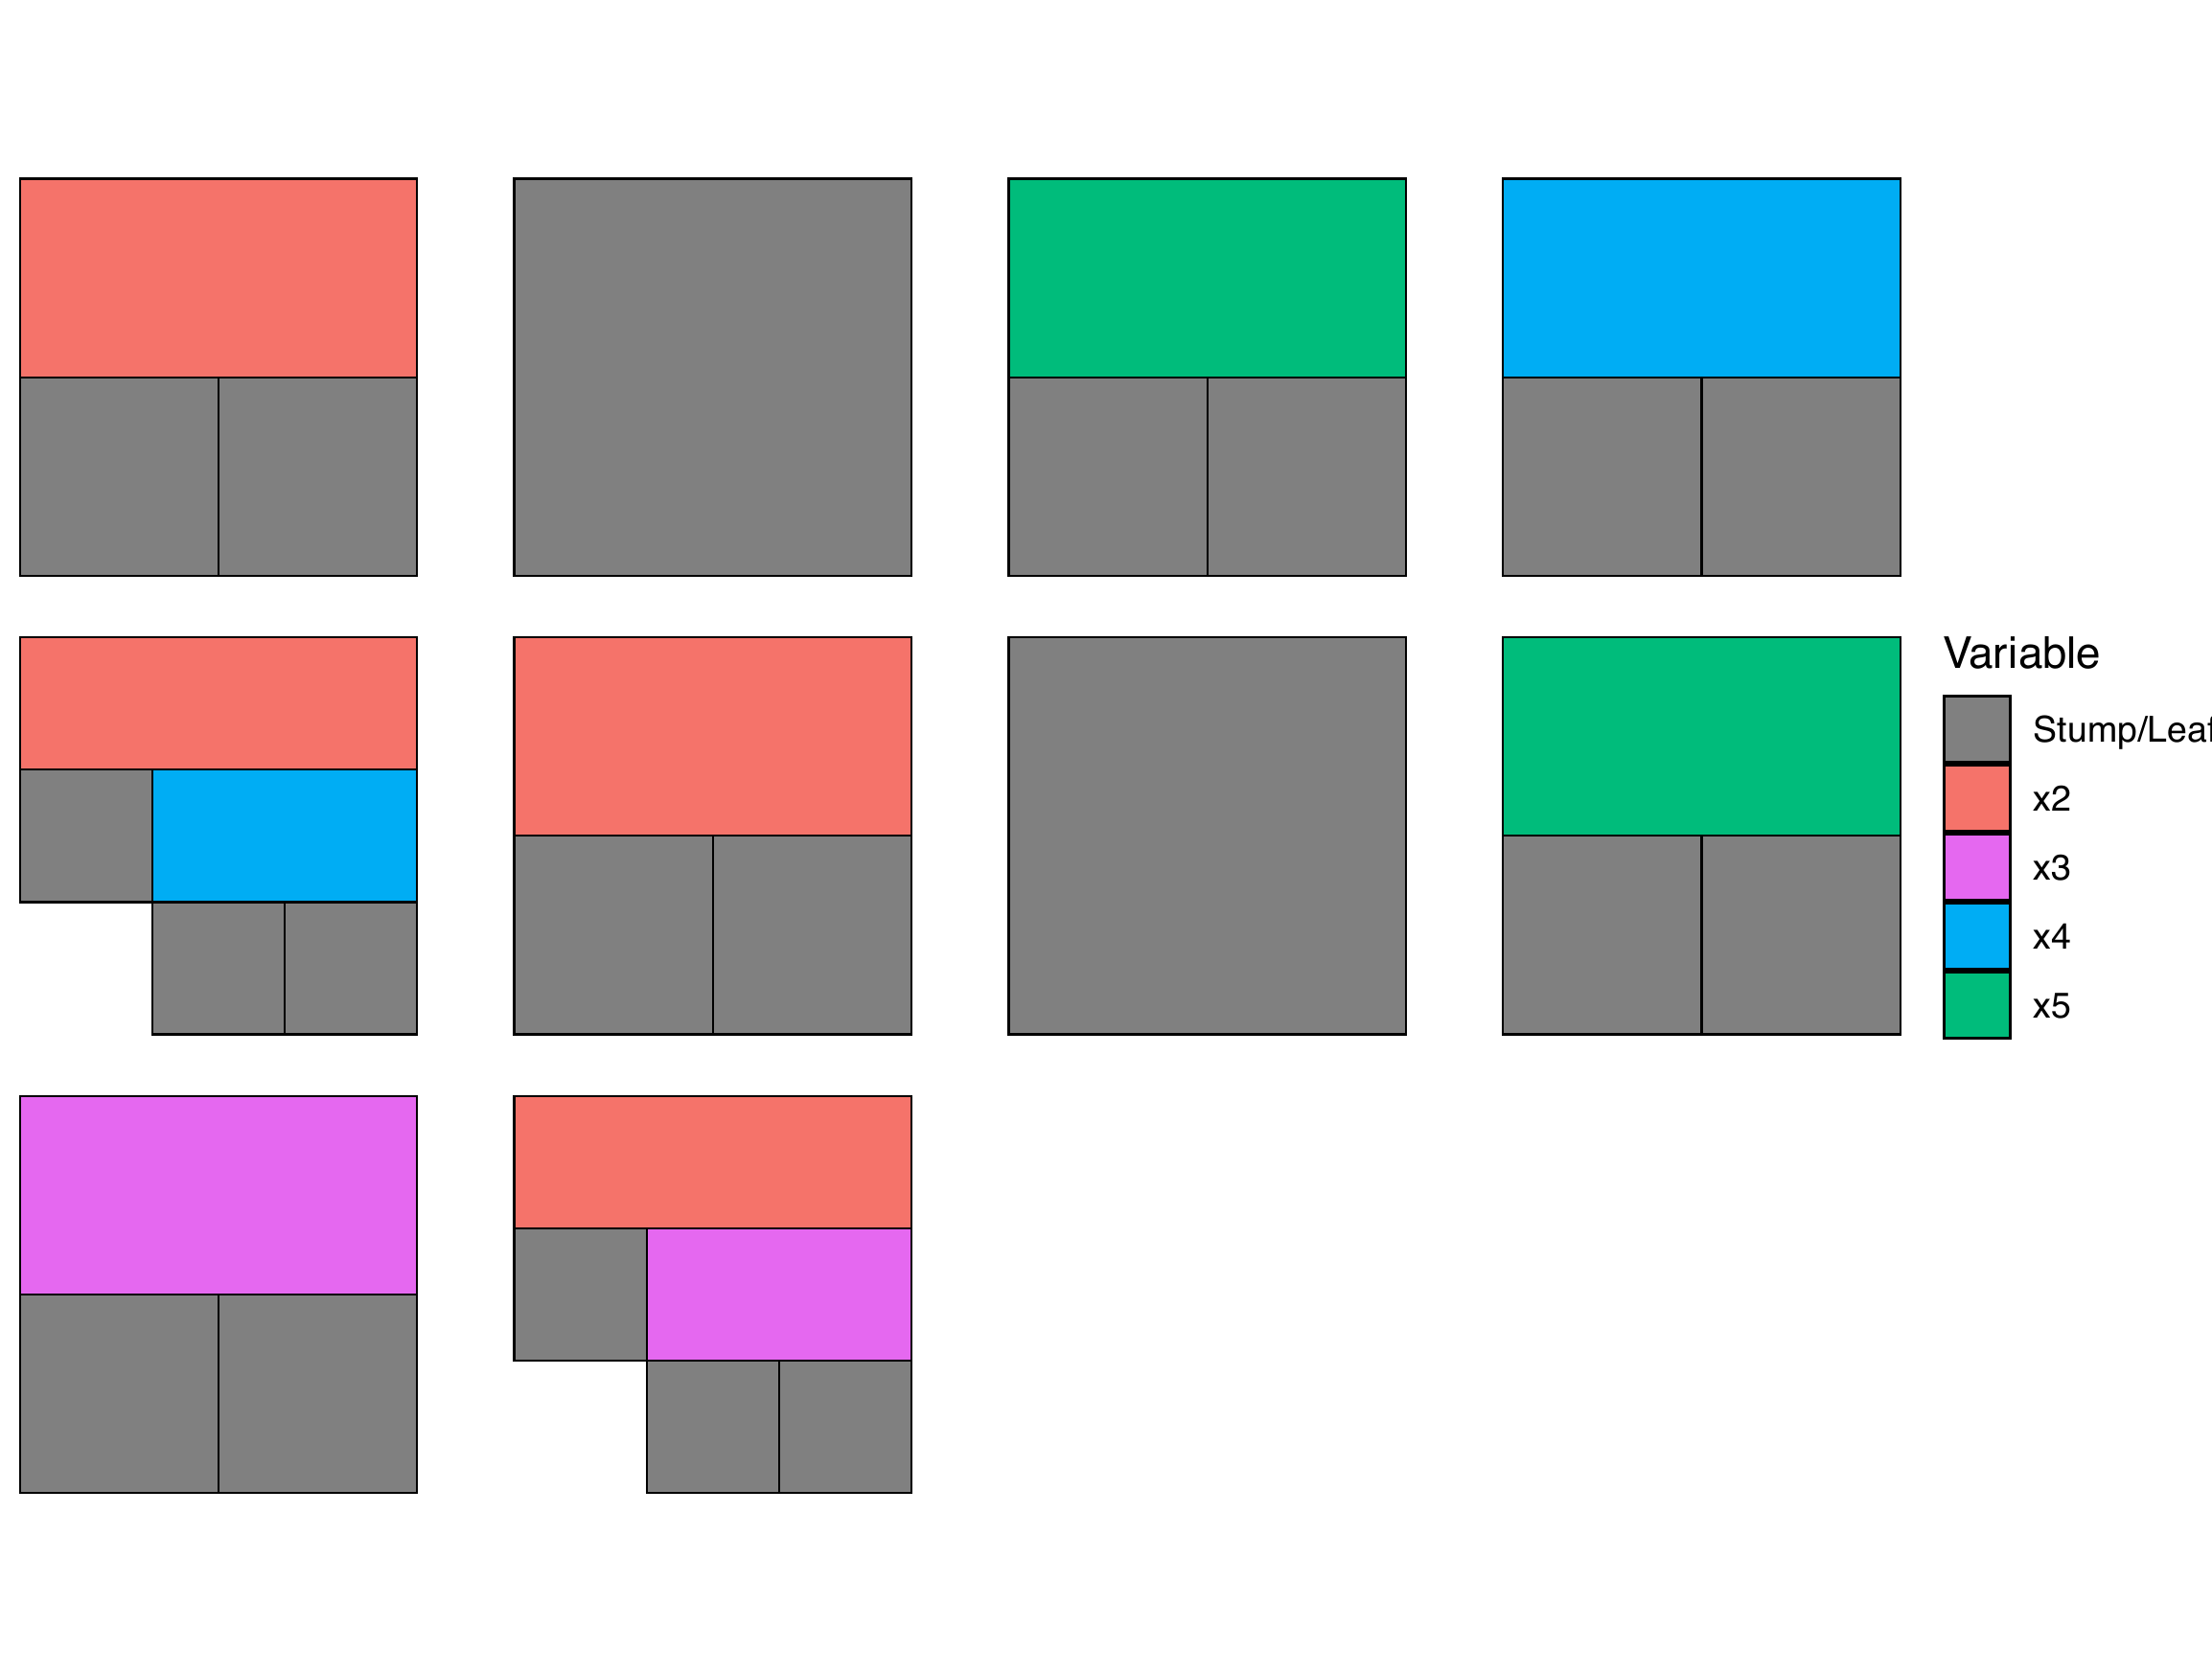
\includegraphics[width=1\linewidth]{https://github.com/AlanInglis/bartMan/blob/master/bartman_vignettte_new_plots_1/own_trees_iter_null_1.png?raw=true
} \end{center}

\protect\hypertarget{fig24:fig24}{}{Figure 24: }stuff here!!!!!

\end{document}
